\documentclass[journal=jacsat,manuscript=article]{achemso}
\usepackage[version=3]{mhchem} % Formula subscripts using \ce{}
\newcommand*\mycommand[1]{\texttt{\emph{#1}}}
\usepackage{graphicx} % Required for inserting images
\usepackage{geometry}
\usepackage[utf8]{inputenc}
\usepackage{helvet} % For custom fonts
\usepackage{setspace} % For line spacing
\usepackage{titlesec} % For title and section customization
\usepackage{etoolbox} % For environment customization
\usepackage{fancyhdr}
\usepackage{xcolor}
\usepackage{ragged2e} % Add this to your preamble for justification options
\usepackage[hidelinks]{hyperref}
\usepackage{amsmath}
\usepackage{chngcntr}
\usepackage{threeparttable}
\usepackage{array}
\usepackage{longtable}
\usepackage{float}
\usepackage{placeins} % ensures centering of your figures
\counterwithout{footnote}{section}

%Subsection settings
\titleformat{\subsection} % Targeting \subsubsection
{\normalfont\normalsize\bfseries} % Font formatting
{\thesubsubsection} % Numbering format
{1em} % Spacing between number and title
{} % Before the title


\author{Raymond D. Cristobal}
\email{rdcristobal@up.edu.ph}
\altaffiliation{These authors contributed equally to this work}
\author{Len Herald V. Lim}
\email{lvlim@up.edu.ph}
\altaffiliation{These authors contributed equally to this work}
\affiliation[University of the Philippines, Diliman]
{Institute of Chemistry,University of the Philippines, Diliman, Quzeon City, Philippines }

\phone{(02) 8981-8500 loc. 3652}

\title[An \textsf{achemso} demo]
{Development of Crude Bit Counting (CBC) and Cluster Subtraction Bit Counting (CSBC) Machine Learning Models: CBC-ML and CSBC-ML For Classification of Molecules Activity Against HCT-116}

\begin{document}
	\maketitle
	
	\begin{abstract}
	In this work we present a method for virtual drug screening based on the use of Morgan Fingerprinting (MFP) and Machine Learning (ML). Two models were created to classify molecular activity against HCT-116. Either model relies on counting of binary-represented molecular fragments generated from MFP, referred to as bits. In Crude Bit Counting (CBC), bits are identified and counted directly based on their absence or presence, while a counterpart method, Cluster-Subtraction Bit Counting (CSBC) pre-classified molecules based on relative activity against HT-116 through clustering before counting bits among clusters. Results show that after coupling with Machine Learning methods (ML), CSBC outperforms CBC based on various parameters pertaining to classification. CSBC-ML has an average accuracy of 94\%, and 98\% for recall, f1 and Area-Under-the-Curve (AUC) score during its training and testing on classifying activity or inactivity against HCT-116. In addition, its ROC curves shows no over-fitting, suggesting robustness. Further inspection of structures classified by CSBC suggests that the clustering stage allows for the consolidation of bits that have similar position and structural environment. These results demonstrated that MFPs generated via CSBC are the best features to use in classifying molecular activity against HCT-116, and that CSBC-ML is a promising method for applications in quantitative structure activity relationship (QSAR).






	\end{abstract}
	\section*{Introduction}
	\setlength{\parindent}{0pt}

Drug discovery is an interdisciplinary and multifaceted field which aims to find new therapeutic agents that could potentially aid or cure a specific disease without detrimental side effects \cite{araujo2018interdisciplinarity}. There are two modes of approach in drug discovery. Traditional methods involve a “trial-and-error” approach, where the discovery of drugs are heavily dependent on natural sources, empirical data, analog design and serendipitous discoveries \cite{article}. An example of this is the study of natural products, which involves the screening of compounds (i.e., extracted from plants, animals, and minerals) against a specific cell-line or bacteria done by Thomford and his co-workers \cite{ijms19061578}. Alternatively, local or internet based chemical libraries are used as a guide on finding drug leads. As an example, the drug design process of Sellamuthu et. al. starts with a known compound exhibiting inherent anti-tuberculosis properties. Based on their design process, an analog was synthesized and subsequently tested against the target cell-line \cite{sellamuthu2023analog}. Notably, the study identified novel lead compounds and uncovered a new therapeutic application. Although traditional methods are proven to work, data shows that the discovery through this path would likely take 10 – 15 years and an average cost of over $1-2$ billion \cite{sun202290}. In addition, it was shown that the number of drugs produced through traditional methods is decreasing, suggesting that it is not sufficient to effectively discover new potential drug candidates \cite{pinzi2024drug} especially in a rapidly scaling economy.  

On the other hand, modern drug discovery methods involve High-Throughput Screening (HTS), Fragment-Based Drug Discovery (FBDD), Structure-Based Drug Design (SBDD), Computational Drug Discovery (CDD), Phenotypic Drug Discovery (PDD), Artificial Intelligence (AI) and ML based techniques \cite{article}. The methods HTS, FBDD, SBDD, and PBDD are known to be experimentally driven while CDD, ML and AI are known to be inherently data driven, computationally intensive and grounded on theoretical principles. \autoref{tab:modern_methods} summarizes their advantages, and their present challenges.  

\begin{table}[h] 
	\centering
	\begin{threeparttable}
		\renewcommand{\arraystretch}{1.2} 
		\small
		\begin{tabular}{p{4cm} p{6cm} p{6cm}}
			\hline
			\textbf{Method} & \textbf{Advantages} & \textbf{Disadvantages} \\
			\hline
			HTS \cite{martis2011highHTS} & Rapid evaluation of compounds for biological activity. Can test up to hundreds of thousands/day.& Expensive cost, requires extensive libraries, suffers from high false-positive rates. \\
			
			FBDD \cite{chen2025fragment} & Narrows down the analysis to small molecular fragments, which results to optimization of potential drugs. & Requires complex strategies and techniques on fragment-linking and advanced structural biology. \\
			
			SBDD \cite{batool2019structure} & Optimizes binding affinity via fitting of drugs to a target. & Availability of high-resolution structural data. \\
			
			CDD \cite{batool2019structure} & Significant reduction of experimental work, cost and time by using simulations and predictive models to screen potential compounds. & Model predictive capacity heavily relies on quality of input data and computational power. \\
			
			PDD \cite{garaci2024PDD} & Focuses on observing changes in disease phenotypes rather than molecular targets. & Mechanistic road map is unclear, requires additional validations. \\
			
			ML \cite{ammad2014integrative} & Flexible and can be combined with different techniques (e.g., QSAR), efficient in predicting drug-targets and molecular properties. & Requires good quality data input, sensitive to imbalanced data set, complexity in integrating to different systems. \\
			
			AI \cite{article} & Automation of drug discovery and other similar systems & Complexity of integration into different systems and difficulty in interpreting and validating predictions. \\
			\hline
		\end{tabular}
	\end{threeparttable}
	\caption{Comparison of modern drug discovery methods} 
	\label{tab:modern_methods} % Fixed label
\end{table}

The effective integration of AI and ML particularly in virtual drug screening, heavily relies on QSAR. QSAR is a computational technique that uses statistical tools to explain the observed structure variation in relation to the target activity \cite{ammad2014integrative}. The crucial step in QSAR is the selection of a good database (e.g., ChEMBL, ChemSpider, DrugBank, and etc) that contains vital information about the candidate molecules. Extracted variables of interest are identified and those posited to notably relate to the target activity are selected. The most common variables used in QSAR are molecular fingerprints. These can be generated through various methods: a) substructure keys-based fingerprints (i.e. MACSS, PubChem fingerprint, BCI fingerprints, etc.); b) topological or path-based fingerprints; and c) circular fingerprints \cite{cereto2015MF}. The selection of an appropriate molecular fingerprint is a pivotal step in QSAR model development as it implicitly dictates the models predictive capacity. Substantial effort is devoted to its optimization and development. 

Substructure keys-based fingerprints use pre-defined structural keys that are matched to a target molecule in a form of binary representations, or bits, \cite{christie1990MACCS}. On the other hand, topological fingerprints uses a linear path in fragmenting a molecule to generate fingerprints. Bits generated from this method might carry more than one meaning if the resolution is not high enough --- a phenomena referred to as bit collision \cite{cereto2015MF}. Circular fingerprints can also be classified as topological fingerprints, with the fundamental difference that instead of using linear paths, the environment of each atom are recorded based on a radial path. The advantage of this technique over the other two are: 1) fingerprints are not fixed, making identification of new meaningful fingerprints possible, and 2) it can detect all of the structural features of a given molecule (i.e., linear and non-linear features) where topological fingerprints fails. This opens up to a higher possibility of detecting new structural patterns \cite{rogers2010extended}. An example of a circular fingerprinting algorithm is Morgan Fingerprinting (MFP) \cite{morgan1965generation}. 

To make quantification possible from the structural queries, similarity analysis is performed via calculation of coefficients. Often used for this purpose are Tanimoto/Jaccard coefficients and Euclidean distances. Observations from these are combined with different mathematical models to create Machine Learning Algorithms (MLA) that can produce accurate and reliable predictions against the target activity \cite{keith2021qSAR}. Unfortunately, the intricacies of the QSAR-ML building procedures, and its creation remains a big challenge \cite{gao2023uni-qsar}.
%Common challenges in traditional methods including: a) identifying viable drug leads; b) reduction of cost, time and experiments demands; and c) improving success rate --- are generally mitigate by modern methods. For instance, HTS, FBDD, SBDD and PDD can experimentally hasten identification of viable drug leads by means of using chemical libraries, structure and phenotypic information. Moreover, experimental demands are significantly reduced and the success rate of drug discovery increases with the aid of AI and ML predictions.

Despite all of the efforts made over the years on drug discovery the following key challenges persist: 1) high experimental and computational demands; 2) difficulty of building a QSAR-ML model that exhibits good predictive capacity against target activity; 3) QSAR - AI/ML integration complexity; and 4) interpretability and validation of results. To address some of these challenges, the current study was aimed at the following objectives: 1) to reduce the complexity of QSAR-ML development by establishing a new method for generating molecular fingerprints; 2) to create a QSAR-ML model that can classify molecular bioactivity using only 2D-structural motifs; and 3) to provide interpretation and validation through structural analysis and random testing. These goals have the following concomitant assumptions: a) there might be molecular fingerprints that directly affect  bioactivity (significant bits); b) the absence and presence of significant bits may also dictate bioactivity; and c) significant bits may incorporate dependency in position and structural environment.    

%The computational work started with no molecular targets set, downloading/scrapping 2D structures of molecules with prescribed bioactivity. This allowed the removal of intrinsic biases and data complexity. From the downloaded 2D structures significant bits are generated via Crude Bits Counting (CBC) and Cluster-Subtraction Bits Counting (CSBC).CBC is a combination of Morgan Fingerprint Algorithm (MFA) and bit frequency counting, wherein it assumes that the most frequently observed bits are responsible for molecules bioactivity. Whereas, in CSBC aside from MFA and bit counting, an extra step of segregation, structure subtraction and bit frequency distribution analysis are performed. These additional extra steps are expected to inherently capture position and neighbor dependencies among the selected significant bits. The generated significant bits from the two methods are used as features for the development of QSAR-ML models: CBC-ML and CSBC-ML. 


%Compared to mentioned modern techniques that entails identifying first the target (i.e., protein, genes and etc), this study propose to not start on any target sites, but instead to start on data base scrapping/downloading of 2D structures with a particular bioactivity. By doing so, it removes prior biases and data complexity. Once the 2D structural and bioactivity information are extracted, molecular fingerprinting via Morgan Fingerprinting Algorithm (MFA) will be applied to generate unique MFP (bits). These bits are hypothesize to contain the significant parts of the compounds that is related to its bioactivity. If correct then, the following are assumed to be true: a) molecules activity is based on the presence and absence of these unique bits, hence, it might be of a high frequency; and b) in case of positional and neighbor dependency, these unique bits might be observe present throughout a given data set. 

%Two methods are develope to extract the molecular fingerprints which are the Crude Bits Counting (CBC) and Cluster-Subtraction Bits Counting (CSBC). CBC involves the logic of linear relationship between the significant bits and target bioactivity, wherein the presence and absence of these bits  are assume to dictates the bioactivity of target compound. On the other hand, CSBC involves segregation of compounds through clustering and structure subtraction. Both CSBC and CBC involves bit frequency counting and ranking  were the top bits were selected based on its frequency in the data set. However, CSBC has an extra step of comparsion to see whether the top candidates are commonly observed across a given data set. Top bits from CBC and CSBC, will be used to QSAR-ML studies, in which two models will be created --- CBC-ML and CSBC-ML. This machine learning models are expected to effectively classify the compounds activity or inactivity against HCT-116. If successfully created, it will be trained and test against molecules with or without bioacitvity against HCT-116. To measure models performance confusion matrix parameters, AUC scores and ROC curve will be used. The best model with a good classification capacity will be recommended for further robust testing.

%HTS is an experimental based approach in drug discovery, which starts on selecting first the target, followed by testing of the compounds coming from chemical libraries, identification hits and drug candidates and finally proceeding to clinical trials \cite{martis2011highHTS}. The main advantage of this method is it offers to test hundreds of thousand of compounds within the span of a day, however, the cost to build the equipment and resources for this method is huge and it suffers from producing false positive and negative errors. 

%Another method that commonly used in drug discovery is FBDD, however, unlike HTS it focuses on small fragments (MW $<$ 300 Da) which potentially have an interaction with the target binding site. Essentially, in FBDD the target binding site is established first followed by creation of small molecule fragments database \cite{chen2025fragment}. These small fragments were test against the target binding site to identify the Ligand Efficiency (LE) and validated through various biophysical, biochemical and computational approach. Once it is validated, the hit will be used to further lead to the optimization of structure and finally development of a drug for a clinical trial. Compared to HTS, FBDD requires fewer number of compounds to find hits and it can also potentially identify novel binding sites. However, the method is quite complex for it involves sophisticated techniques such as NMR and X-ray crystallography. Moreover, analysis of binding affinity of small molecule fragments to binding site is often hard for its signal is weak and almost comparable to noise. 

%SBDD starts on generation human genome sequence, followed by extraction of proteins, and then from there, the therapeutically important proteins are identified and their structure gets elucidated. After, the preparation of active compounds database takes place and the identification of druggable target protein and its binding sites. Consequently, the screening and docking of active compounds against the binding cavity of target protein are performed. Results from screening and docking hits will be rank based on their binding affinities, and the top compounds are selected to proceed to synthesis and clinical trials \cite{batool2019structure}.

%CDD is essentially combination of SBDD and Ligand-Based Drug Discovery (LBDD). Known protein structure and ligands are assessed and hit against the database of active compounds, through this method, virtual screening takes place and the hits are identified. After, molecular docking and dynamics are performed to verify the interaction and identify the LE of the hits. Lastly, quantitative structural activity relationship (QSAR) modelling is created, which is later used to generate prediction with regards to the bioactivity of the compound against the target site \cite{schaduangrat2020CDD}. The main advantage of this technique over the experimental-based (e.g., HTS, FBDD, SBDD, and PDD) is that it streamlines the procedure of drug discovery with lesser cost and reduced physical testing. 

%PDD is a method that identifies small molecules or peptides that possibly alter the desired phenotype of cell organisms. Generally, PDD method starts on selection of model system, which should be ideally closely or totally reflects the phenotype of target disease. After selection, development of assay takes place wherein it involves measuring cell viability, changes in protein expression and etc. When development of assay is successful, compounds from libraries will be screened against it to identify which changes the phenotype significantly. Once there is a hit, lead compound will be validated through testing the model system with its various concentration. Validated hits will undergo mechanism studies to understand and identify the interaction between the compound and the biological target(s). Despite the laborious task of assaying, PDD offers to unveil novel and complex mechanism of compounds against complex biological system of target cells. Conversely, since the PDD method does not require prior knowledge to exact biological targets, its identification poses a challenged, which lead to extensive testing and verification \cite{garaci2024PDD}. 

 






	
	\section*{Results}
	\subsection*{SAR: MFP and \% Inhibition HCT-116}
\begin{figure}[htbp!] % 'h' places the figure approximately here
	\centering
	\hspace{-1cm}
	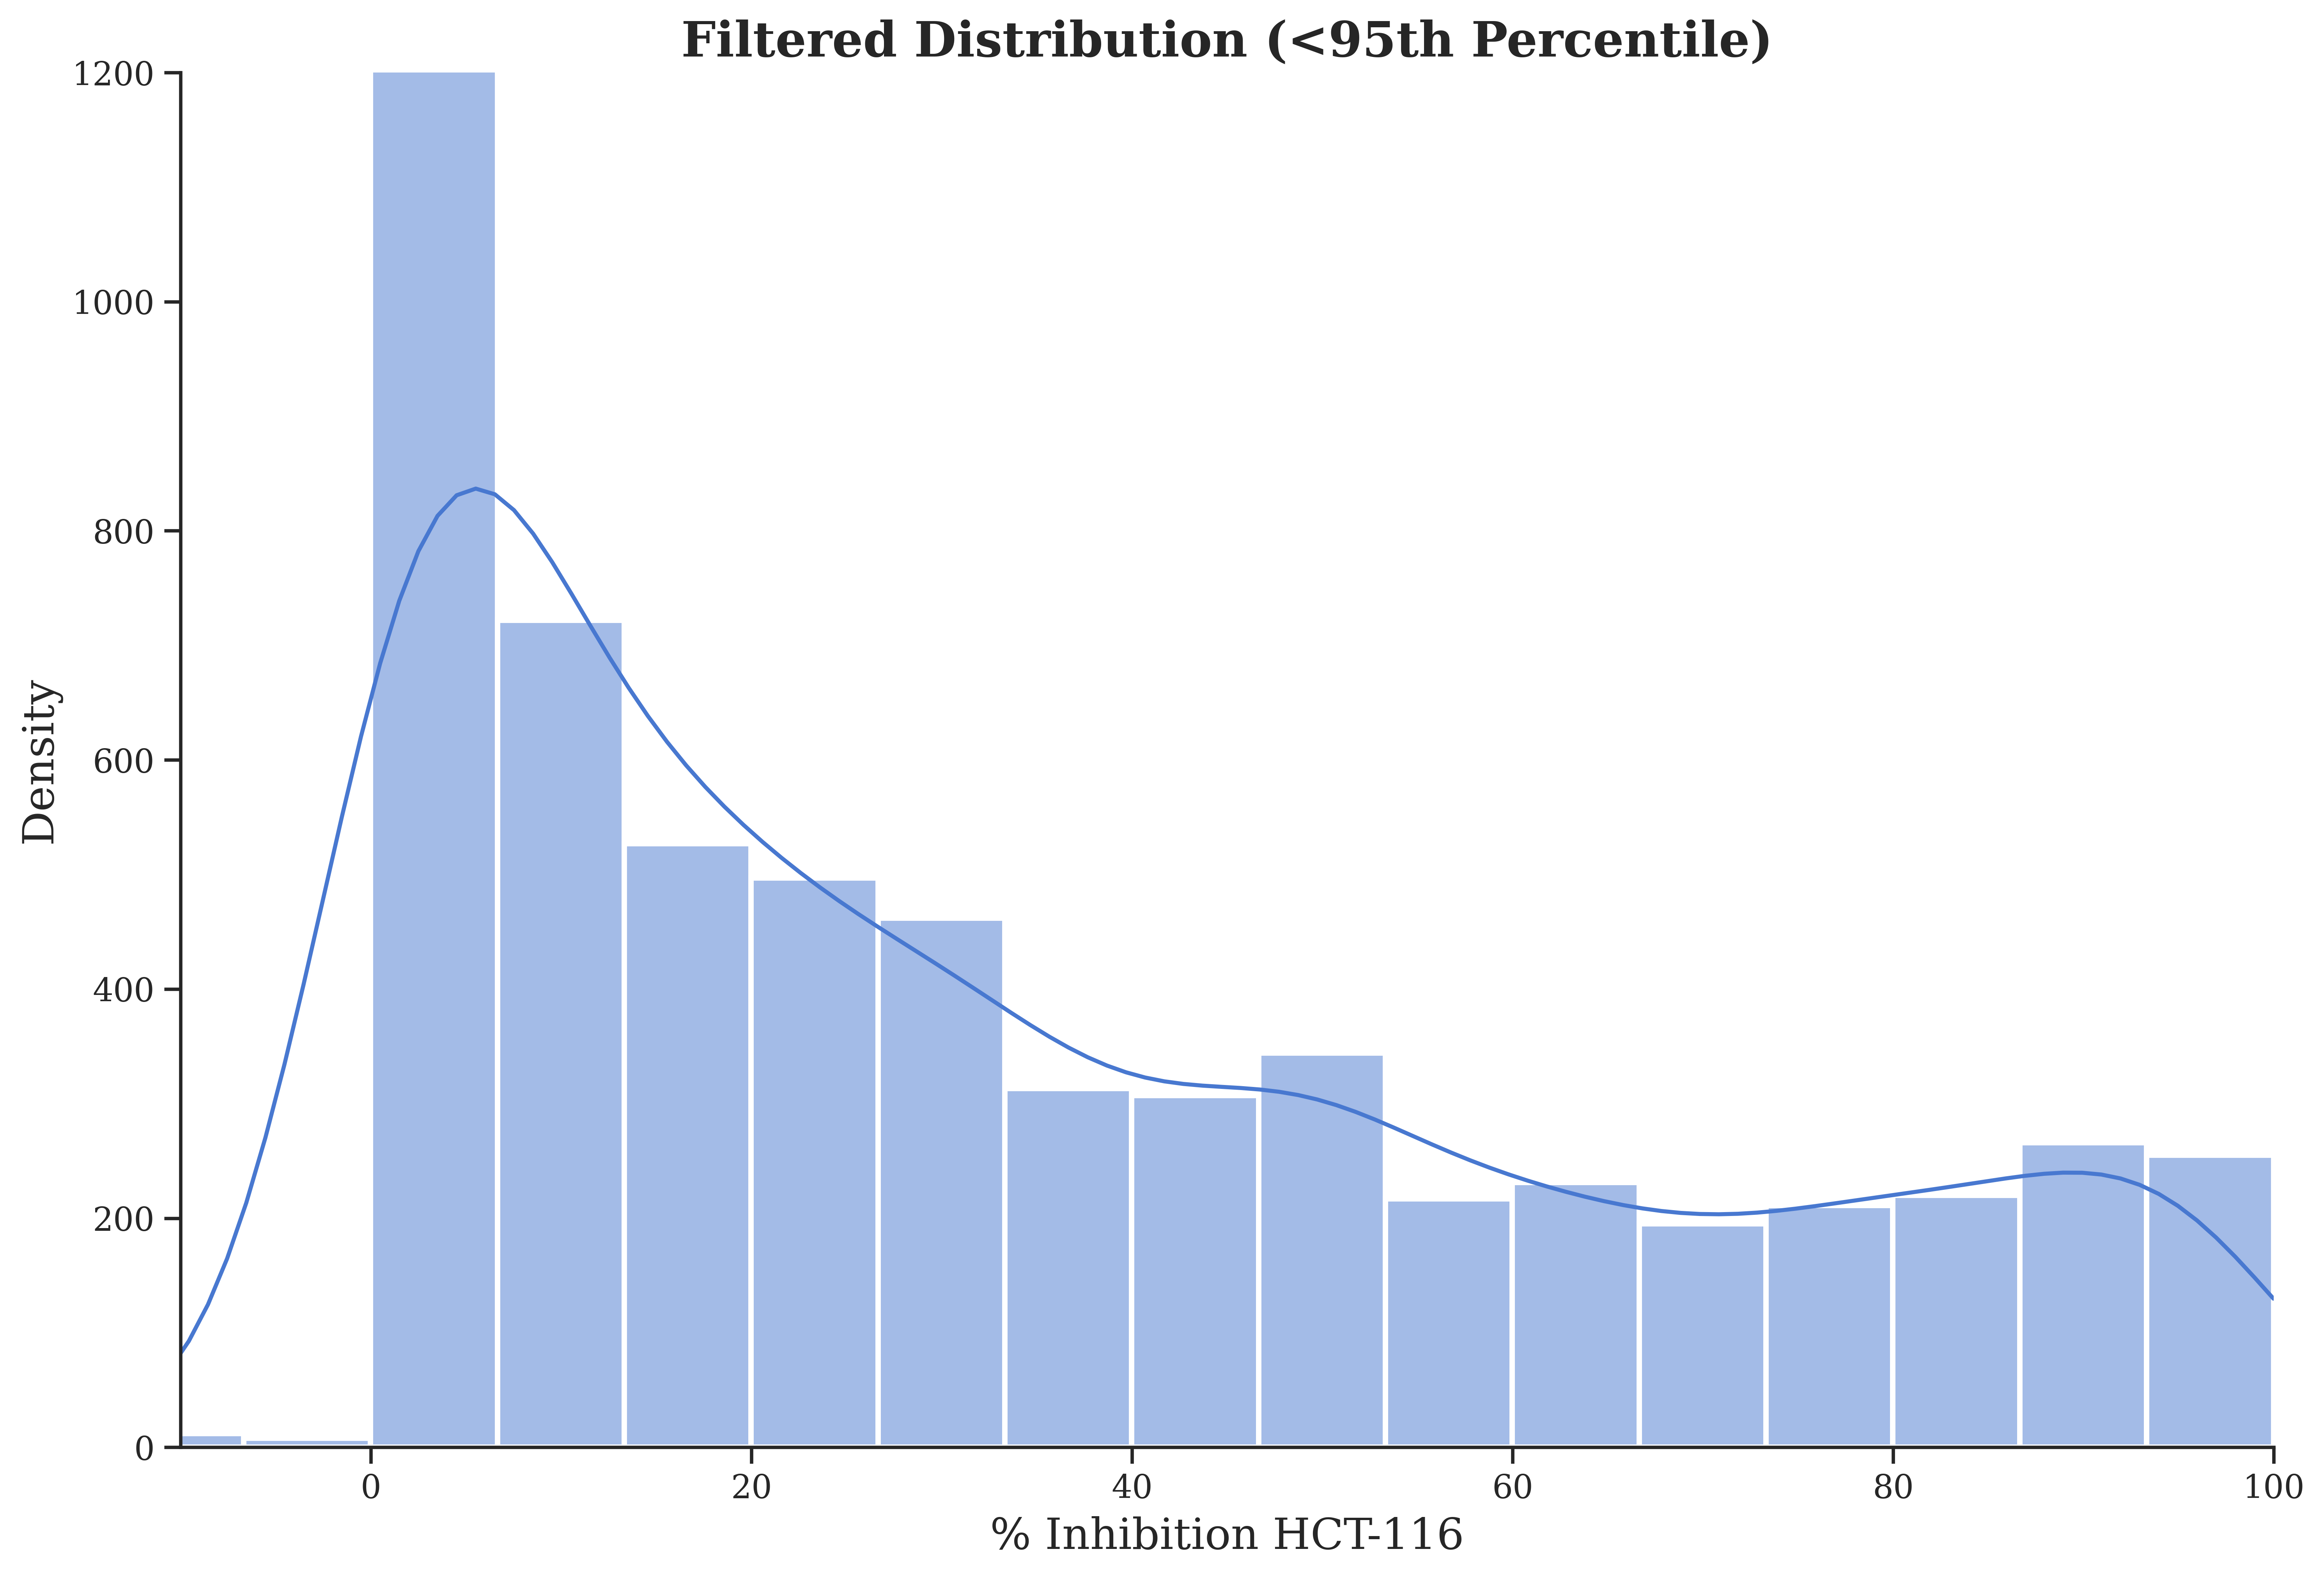
\includegraphics[width=0.8\textwidth]{cleandatadist.png}% Replace with your image filename
	\caption{Distribution of clean dataset of HCT-116}
	\label{fig:cleandist} % Optional: use \label for referencing
\end{figure}

Development of ML models are heavily dependent on the data quality \cite{zhou2024dataquality}. Erroneous and misleading predictions generated by the models are often associated with outliers that were not removed during the training and testing period. Unfiltered dataset was observed to have 70.16 skewness, indicating that most of the data outliers are located on the positive tail end of the curve. If not removed, it is expected to result in positive errors in predictive models. Thus, the dataset used in this study was pre-processed prior to modelling, resulting to filtered data that has a  skewness of 0.05386, leading to a significant improvement in distribution. \autoref{fig:cleandist} shows that filtered/clean data has an asymmetric normal distribution (i.e., imbalanced data set). SMOTE serves to balance the minority and majority class of the data set, removing positive biases in model predictions (\autoref{fig:SMOTE}).

\FloatBarrier
\begin{figure}[h]
	\centering
	\begin{minipage}{\textwidth}
		\centering
		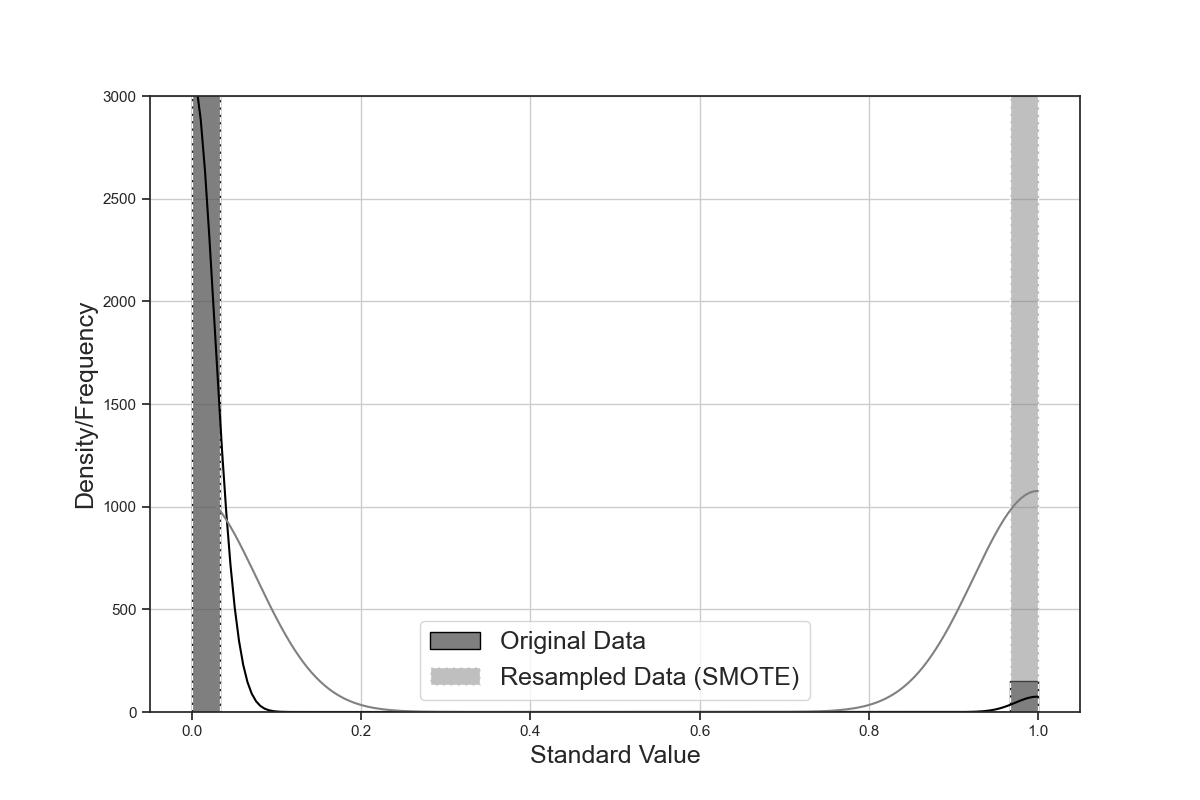
\includegraphics[width=1\textwidth]{SMOTEbw.png}
		\vspace{-1cm}
		\caption{Comparison of distributions before and after SMOTE}
		\label{fig:SMOTE}
	\end{minipage}
\end{figure}
\FloatBarrier

%\begin{figure}[htbp] % 'h' places the figure approximately here
%\centering
%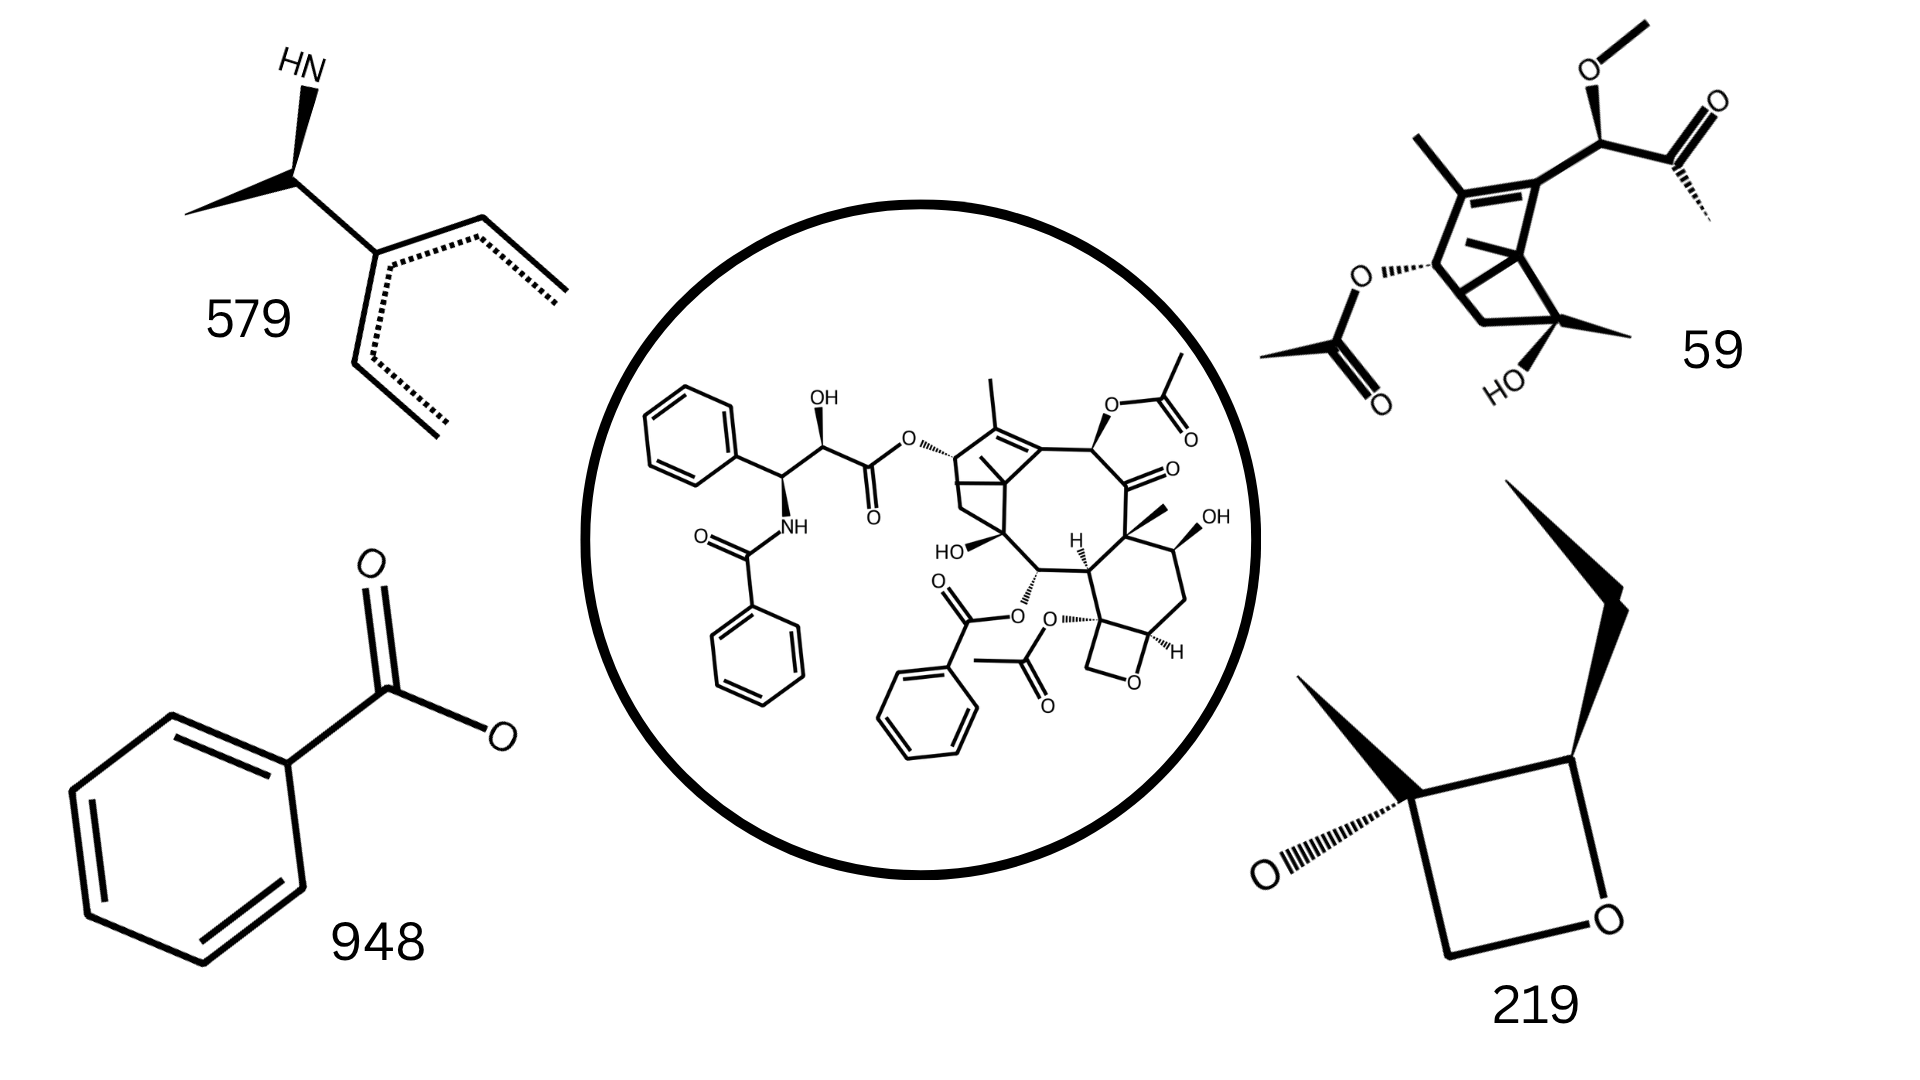
\includegraphics[width=0.7\textwidth]{fragmentation.png}% Replace with your image filename
%\caption{Fragmentation of Target Compound to Produce MF and Bit Number Assignment}
%\label{fig:mfex} % Optional: use \label for referencing
%\end{figure}

The MFA produced a maximum of 2048 bits for each compound and approximately 12 million bits in total were analyzed in this study. \autoref{tab:summary} presents the summary of pre-processing and generation of MFPs and MPs from MFA. The CBC method revealed that there are bits that were frequently present in molecules with or without bioactivity against HCT-116. \autoref{fig:top10crudebits} shows the top 10 bits observed through CBC. Nearly all of the top 10 bits identified from CBC can be considered as small fragments. Changes in these bits could lead to positive or negative effects to bioactivity (\autoref{fig:top10crudebits}). Since the bits were not segregated and non-significant bits were not removed prior to bit frequency counting, it is possible that the identified top 10 bits represents a mixture of positive, negative and non-significant bits. 
%To perform QSAR studies of the given clean data set, the generation of MF's plays the pivotal role on giving the MFA its capacity to perceived structural patterns in a binary format.  

%To gain a meaningful structural insight, the CBC and CSBC were employed. In essence, the presence and absence of particular bits and its relation to \% Inhibition can be simply detected by means of counting its frequency. This simple logic was leveraged in CBC method, wherein after the generation of MP's and MF's of the compounds, bit of a specific MF's were counted and ranked (see \autoref{tab:t10crude}). Essentially, the MF with highest bit frequency were expected to have a relationship with the \% Inhibition of compounds against HCT-116. On selecting the top 10 bits, researchers set the frequency values to at least 50\% of the total data, assuming that it is equal to the amount of observation that has a significance.

\begin{table}[h] % Optional: for floating the table
	\centering
	\begin{threeparttable}
		\renewcommand{\arraystretch}{1.2} % Adjust row spacing (1.2x normal)
		\small
		\begin{tabular}{p{3cm} p{4cm} p{4cm} p{2cm} p{2cm}} % Five columns (all centered and with vertical borders)
			\hline
			Molecule ChEMBL ID & SMILES & Mols \tnote{a} & \%Inhibition & MP \\ 
			\hline
			CHEMBL259084 & O=C(O)c1ccc$\ldots$ & rdkit.Chem.rdchem.Mol object at 0x00000225A15$\ldots$ & 6.400 & 111010101$\ldots$ \\ 
			CHEMBL224940 & CCCCN1CCN(C(=O)$\ldots$& rdkit.Chem.rdchem.Mol object at 0x00000225A15$\ldots$ & 27.000 & 101110100$\ldots$ \\ 
			CHEMBL2029910 & CN1CCN(C(=O)c2cc$\ldots$ & rdkit.Chem.rdchem.Mol object at 0x00000225A15$\ldots$ & 0.003 & 101010100$\ldots$ \\ 
			\vdots & \vdots & \vdots & \vdots & \vdots \\
			CHEMBL3813873	 & FC(F)(F)c1ccc$\ldots$ & rdkit.Chem.rdchem.Mol object at 0x00000225A16$\ldots$ & 4.280 & 111110101$\ldots$ \\ 
			\hline
		\end{tabular}
		\begin{tablenotes}
			\item[a] Mols indicates molecular object data type which is interpreted as a display or png file by the rdkit package. 
		\end{tablenotes}
	\end{threeparttable}
	\caption{Summary of data profiles for compounds}
	\label{tab:summary}
\end{table}

\begin{figure}[htbp!] % 'h' places the figure approximately here
	\centering
	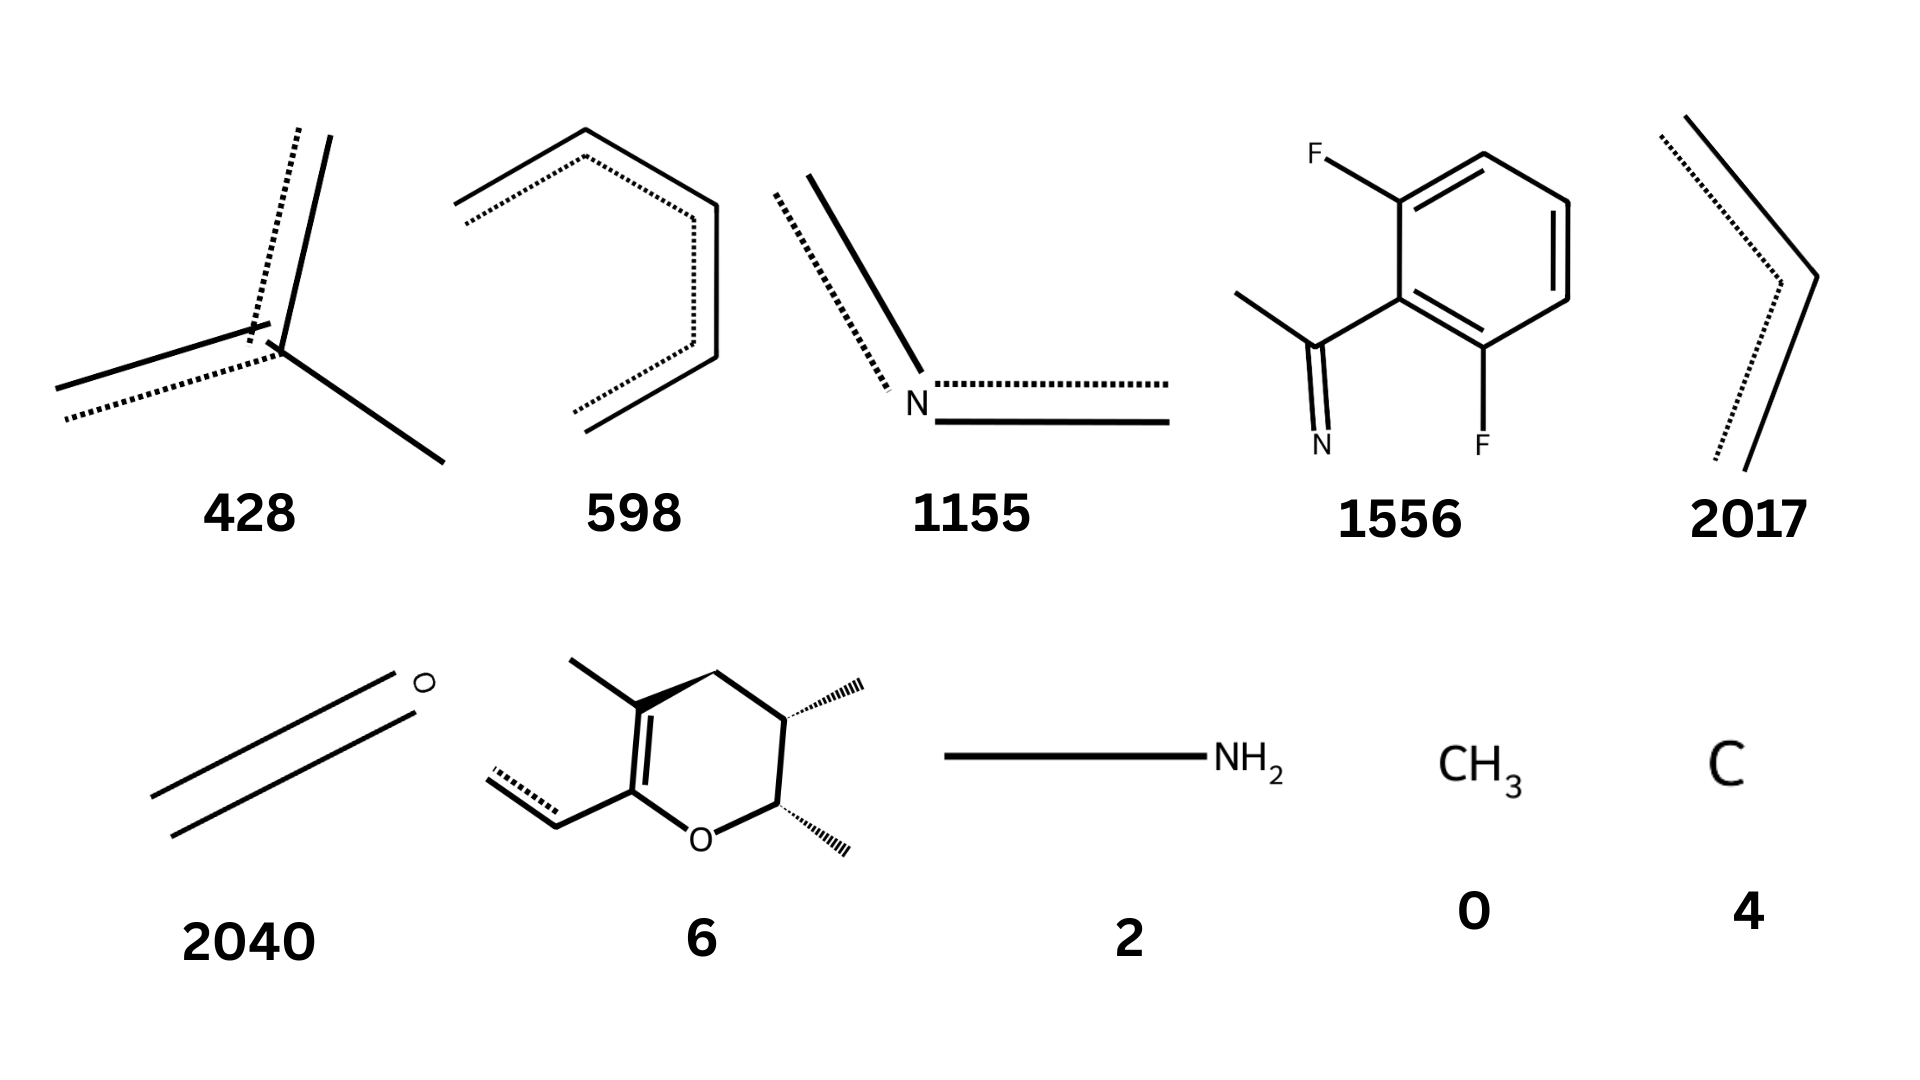
\includegraphics[scale=0.30]{top10crudebitsv2.png} % Replace with your image filename
	\caption{CBC top 10 bits: 2D - structures}
	\label{fig:top10crudebits} % Optional: use \label for referencing
\end{figure}

%Based on the results CBC identified the following bits: 0, 2, 4, 2017, 2040, 428, 6, 1556, 1155, and 598 as significant bits. Wherein, the algorithm suggest that these bits have a significant relationship with the bioacitivity of compounds. The machine 2D perception of the bits are quite unique, for it accounts the following: a) central atom (colored with blue dots); b) atomic substitution (color yellow)\footnote{yellow color represents sulfur substitution or other electronegative atoms}; and c) predicted bonds at the end of structure (colored with gray)\footnote{dashed grey line represents partial bonds}. Structurally, almost all of them were considered to be a small fragments, this could mean that structural or conformational changes in this bits could lead to inactivity of a compound (\autoref{fig:top10crudebits}). However, it was assumed that since the bits were not segregated and non-significant bits are not removed prior to bit frequency counting, probably the constituents of Top 10 bits from CBC could have a mixture of positive, negative and non-significant bits. To verify this assumption, the identified structural features will be used in the creation of CBC-ML, wherein the machine will be train and test to classify compounds activity based on the input features extracted from this method.  

The CBC method is a simple technique to identify the significant bits from the clean dataset, but it does necessarily incorporate information on the position and neighboring structural motifs. Therefore, there may be cases that the presence or absence of a particular bit will have different meanings depending on their position or structural environment. In contrast, because CSBC employed blind clustering, it allows for the categorization of data prior to counting. This intermediate step gives an insight on the different clusters that exist in the given dataset, which could lead to classification and discovery of new structural patterns. One underlying assumption in the application of CSBC is that common features shared among clusters will implicitly incorporate the dependence on position and neighborhood of structural motifs. Furthermore, subtraction of clusters  may naturally remove non-significant bits which could lead to more efficient identification of positively and negatively contributing bits. 

%several critical factors to understand and accurately classify the compounds based on their structural features. The researchers identified these critical factors to be the position and neighbor of bits. The algorithm used in CBC does not take into account where does the bits located and what are its neighbors during the counting process. Therefore, it is probable that there will be cases that the presence or absence of a particular bit will have different meanings depending on their position or neighbor. To mitigate this possibility, another method is developed to account these kind of scenarios which is called CSBC. In CSBC, blind clustering was first employed prior to counting, this was done to segregate the data sets and simplify it prior to counting. This intermediate step gives an insight about the different clusters that exist in the given data set that could lead to classification and discovery of new structural patterns. Essentially, the researchers assumed that, these clusters of compounds will have something in common and different, therefore, if these information could be extracted, probably the dependency in position and neighbors of the compounds could be understood. Furthermore, researchers also assumed that by doing blind clustering the presence of non-significant bits could be removed giving a way to identify early on the positive and negative bits. 

Result shows that the optimum number of clusters for the given data set using the Elbow Method is 5. K-Clustering divided 6304 \% Inhibition data into 5 categories which were classified as: a) HI (purple); b) MI (blue); c) LI (orange); d) VLI (green); and e) NI (red) (\autoref{fig:cluster}). The VLI region in contains the compounds with \% Inhibition of around -20 to 20, and it can be considered as the neutral point of the bioactivity \footnote{region of the dataset that could be regarded as having non-significant bioactivity or close to 0 \% Inhibition} (\autoref{fig:cluster}). The structural features of compounds under this category may considered to be non-significant and must be removed. In addition, it is also assumed that from the set neutral point going up and down to HI and NI respectively may mean that alteration of molecular structures in these regions might lead to maximization or minimization of bioacitivity against HCT-116. Therefore, subtraction of molecular MPs in the VLI region from those in the HI, MI, LI, and NI regions may lead to the extraction of structures that either increase or decrease their bioactivity.        

%\begin{figure}[h] % 'h' places the figure approximately here
	%\centering
	%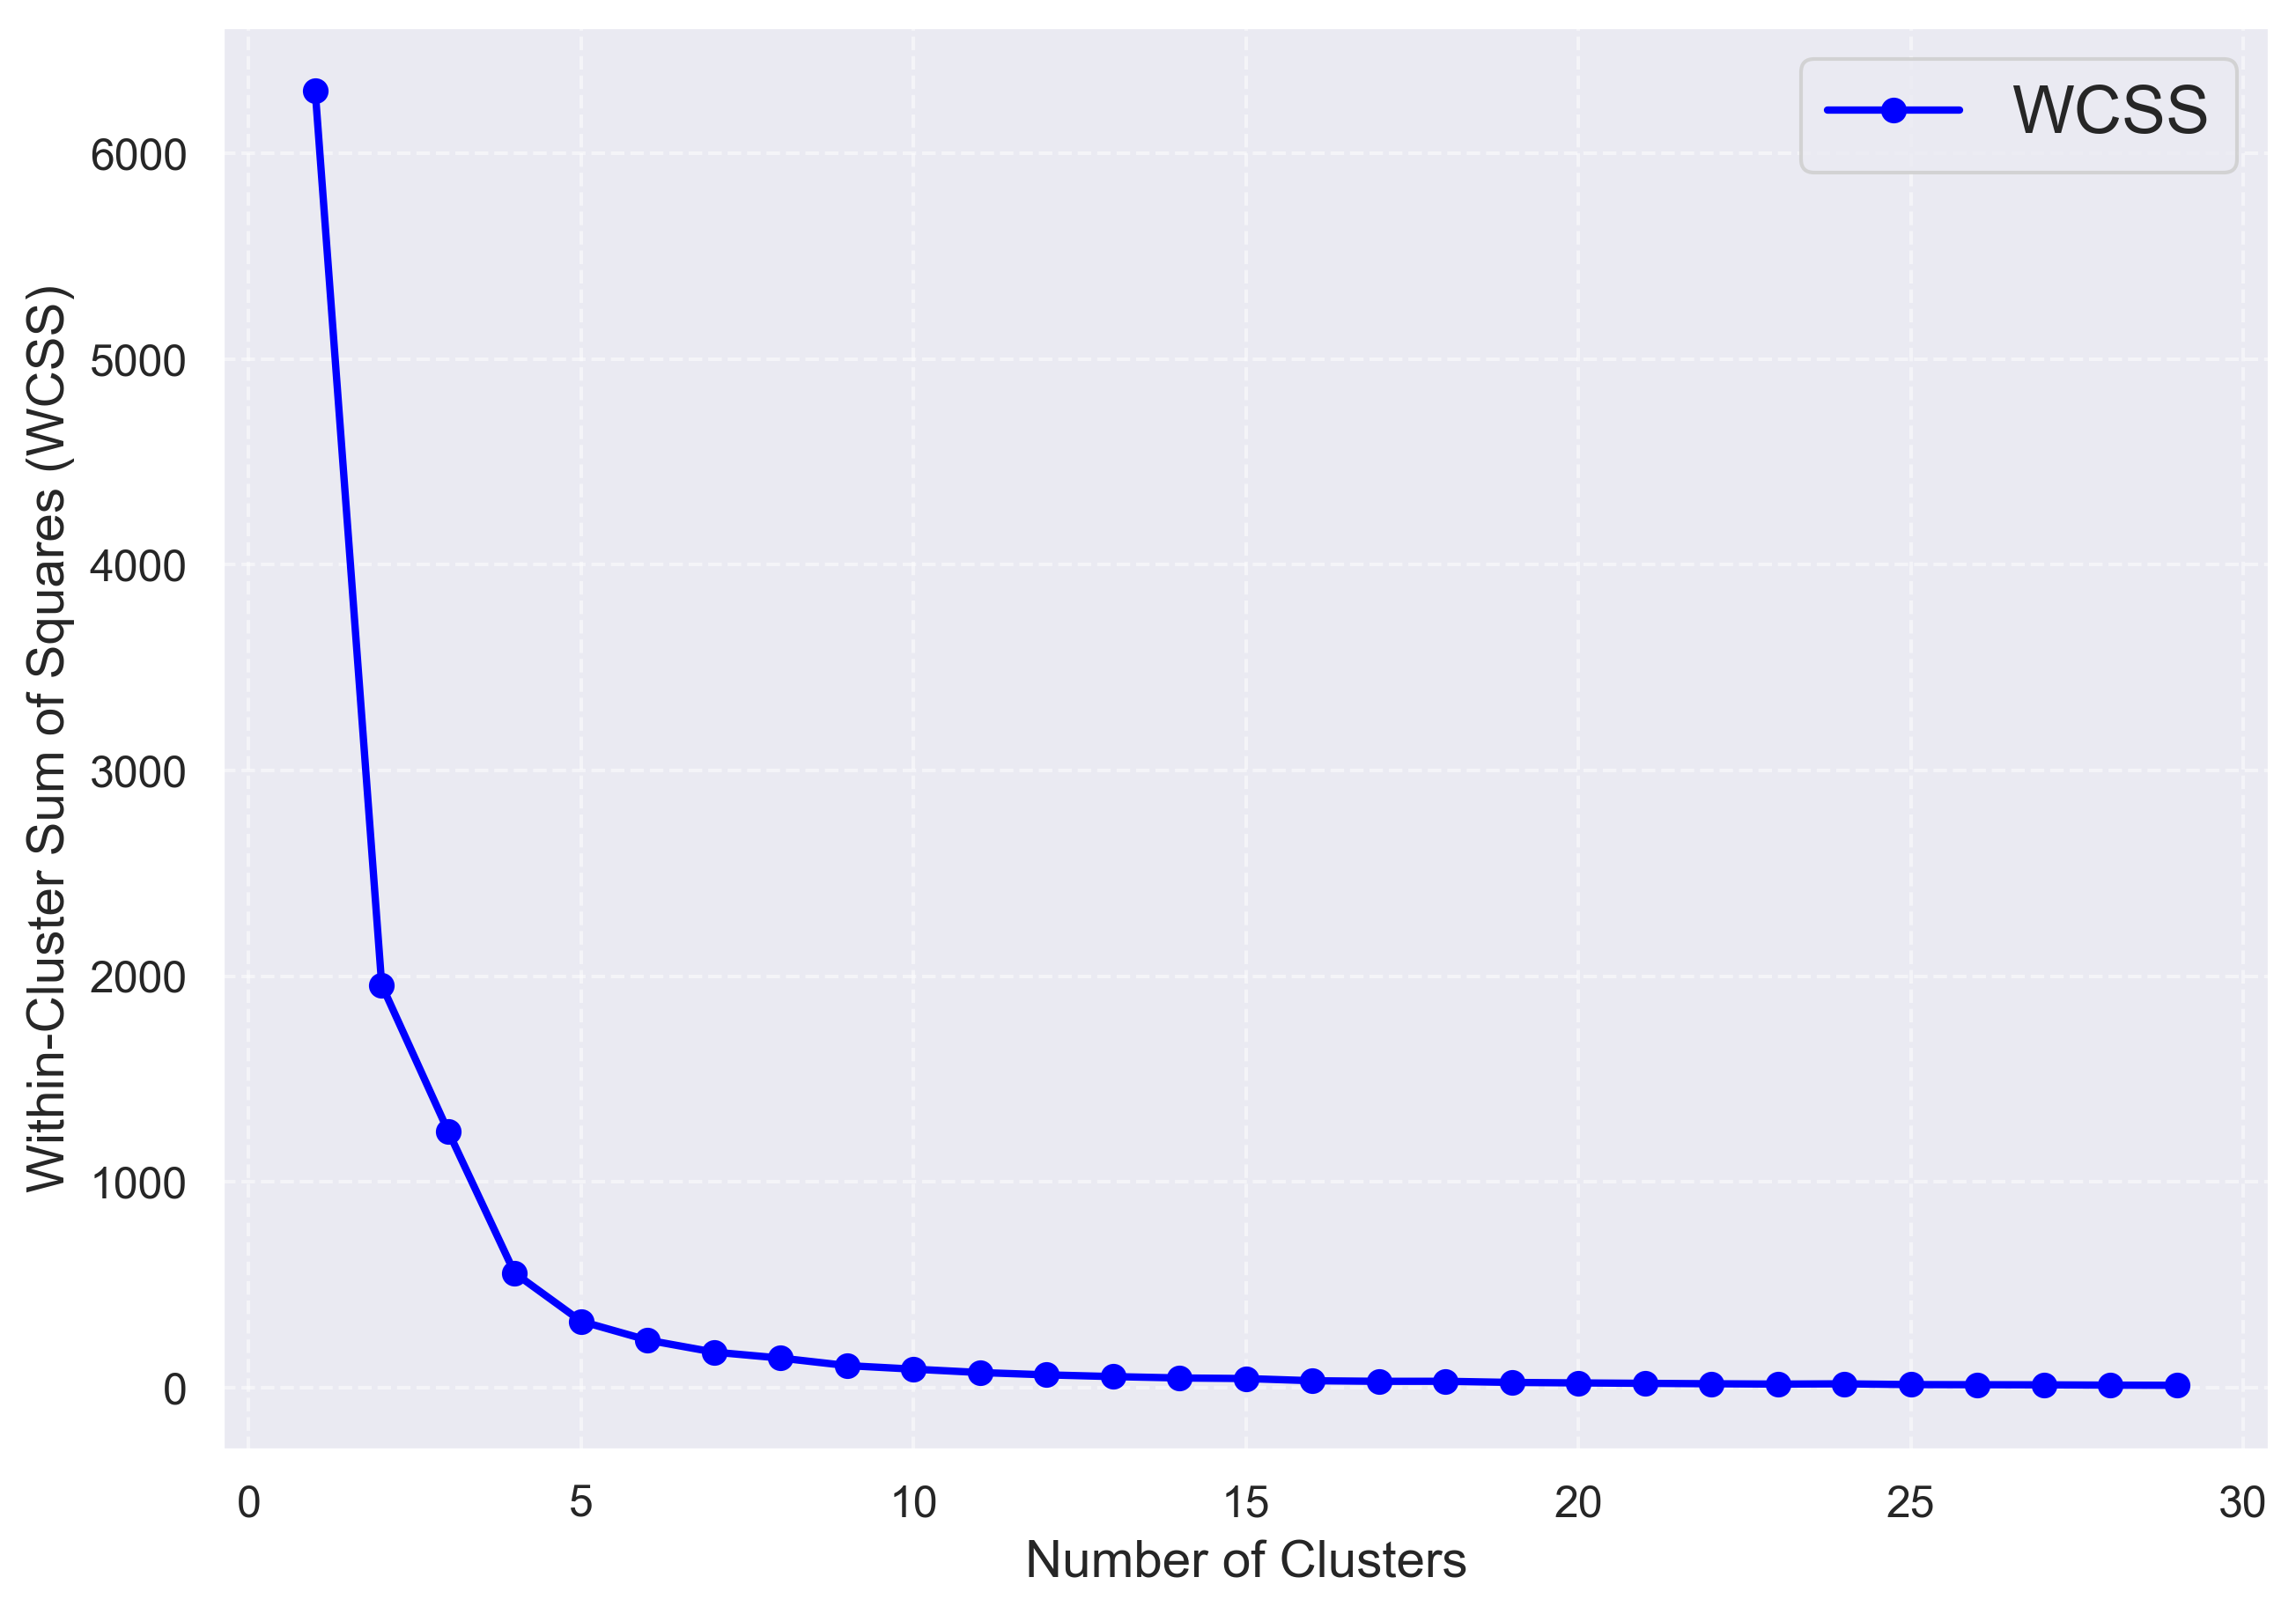
\includegraphics[width= 0.9\textwidth]{elbow.png} % Replace with your image filename
	%\caption{Elbow Method for Optimal Number of Clusters}
	%\label{fig:elbow} % Optional: use \label for referencing
%\end{figure}


\begin{figure}[h] % 'h' places the figure approximately here
	\centering
	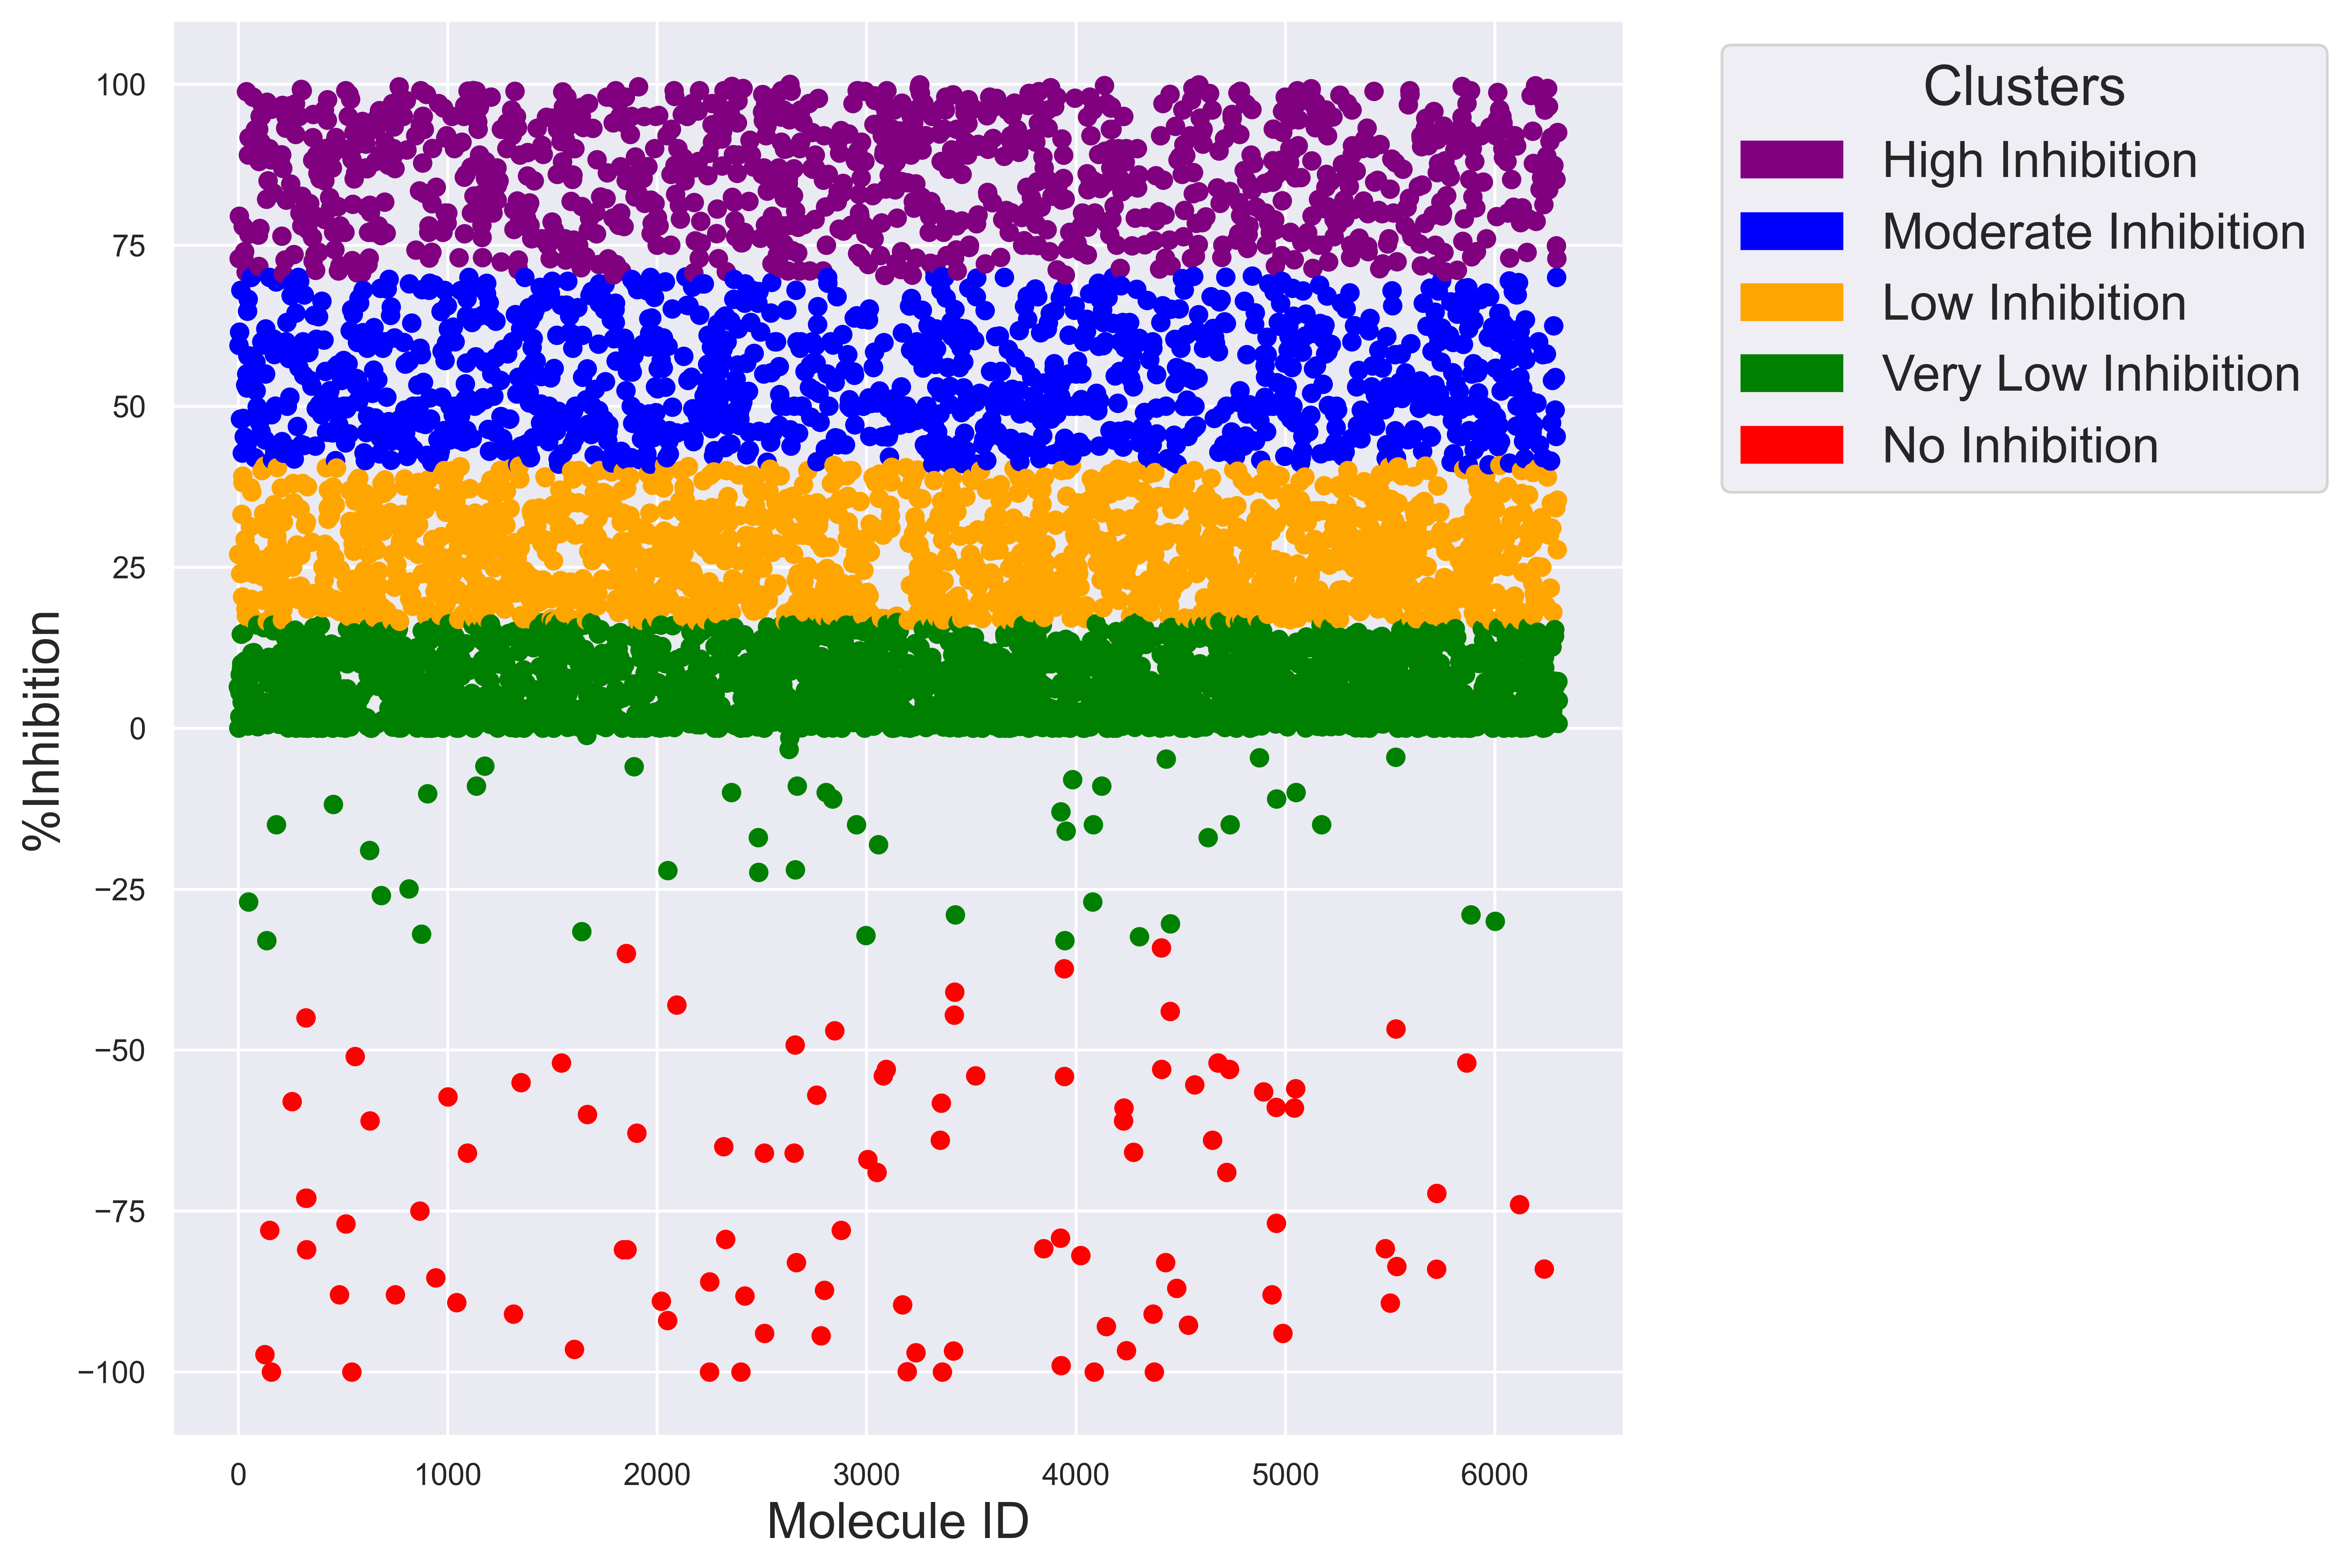
\includegraphics[scale=0.6]{cluster.png} % Replace with your image filename
	\caption{Cluster analysis of bioactivity against HCT-116}
	\label{fig:cluster} % Optional: use \label for referencing
\end{figure}

HI, MI, LI, VLI and NI have the matrix dimensions of (1035 x 2048), (1162 x 2048), (1588 x 2048), (2417 x 2048), and (102 x 2048) respectively. The entire process of VLI subtraction to all categories results to a total of 9,394,879 newly formed MPs removing approximately 3,515,713 non-significant MFs. These new MPs that essentially contain the PBs and NBs were simplified by means of combining similar MPs and counting their frequencies. From this process, the PBs and NBs were identified based on their relationship with \% Inhibition against HCT-116, ranked based on frequency, and compared to identify commonalities. The summary of top bits is shown in \autoref{fig:mostcombits}. It must be noted that the resulting difference between VLI-HI and VLI-NI were considered to be positive and negative bits. Whereas, the results from VLI-MI and VLI-LI differences were considered to be moderate bits. In addition, it was observed that there were common bits among the results within differences. It is then a matter of investigating these common bits to verify whether there is a considerable degree of retention on position and neighborhood dependency.

%These findings could imply that there could be a position or neighbor dependency among the observed bits, which probably explains its presence among all the clusters.


%mentioned bits were observed on the compounds with high, moderate, low, and negative bioactivity against HCT-116. Hence, it implies that these bits could be position or neighbor dependent. This implication explains why these bits were present on the compounds with high, moderate, low and negative bioactivity. These implications can be verified through the development of CSBC-ML, wherein the input features to be used are the bits generated from CSBC.


Most of the common bits were found to correspond to small molecular fragments. A close inspection of these bits offer some interesting observations. For instance, bit 857 and 428, are mirror images of each other, and are non-superimposable, reavealing that they are enantiomers. In addition, bits (1155, 2039), (1863, 1917) are constitutional and functional isomers. This small detail of change in conformation, connectivity and functional groups where detected through the use of CSBC method (\autoref{fig:mostcombits}). Hence, it is expected that it will have different weights when used in CSBC-ML. 
%Observing the structures of bits 857 and 428, notice they are mirror images of each other,however,they are non-superimposable, hence they are enantiomers. In addition, bits (1155, 2039), (1863, 1917) are constitutional and functional isomers.This small detail of change in conformation, connectivity and functional groups where detected through the use of CSBC method. Therefore, when these structural features are use in the model of CSBC-ML, it is expected to have different weights.      
%\FloatBarrier
%\begin{figure}[h]
	%\centering
	%\begin{minipage}{\textwidth}
		%\centering
		%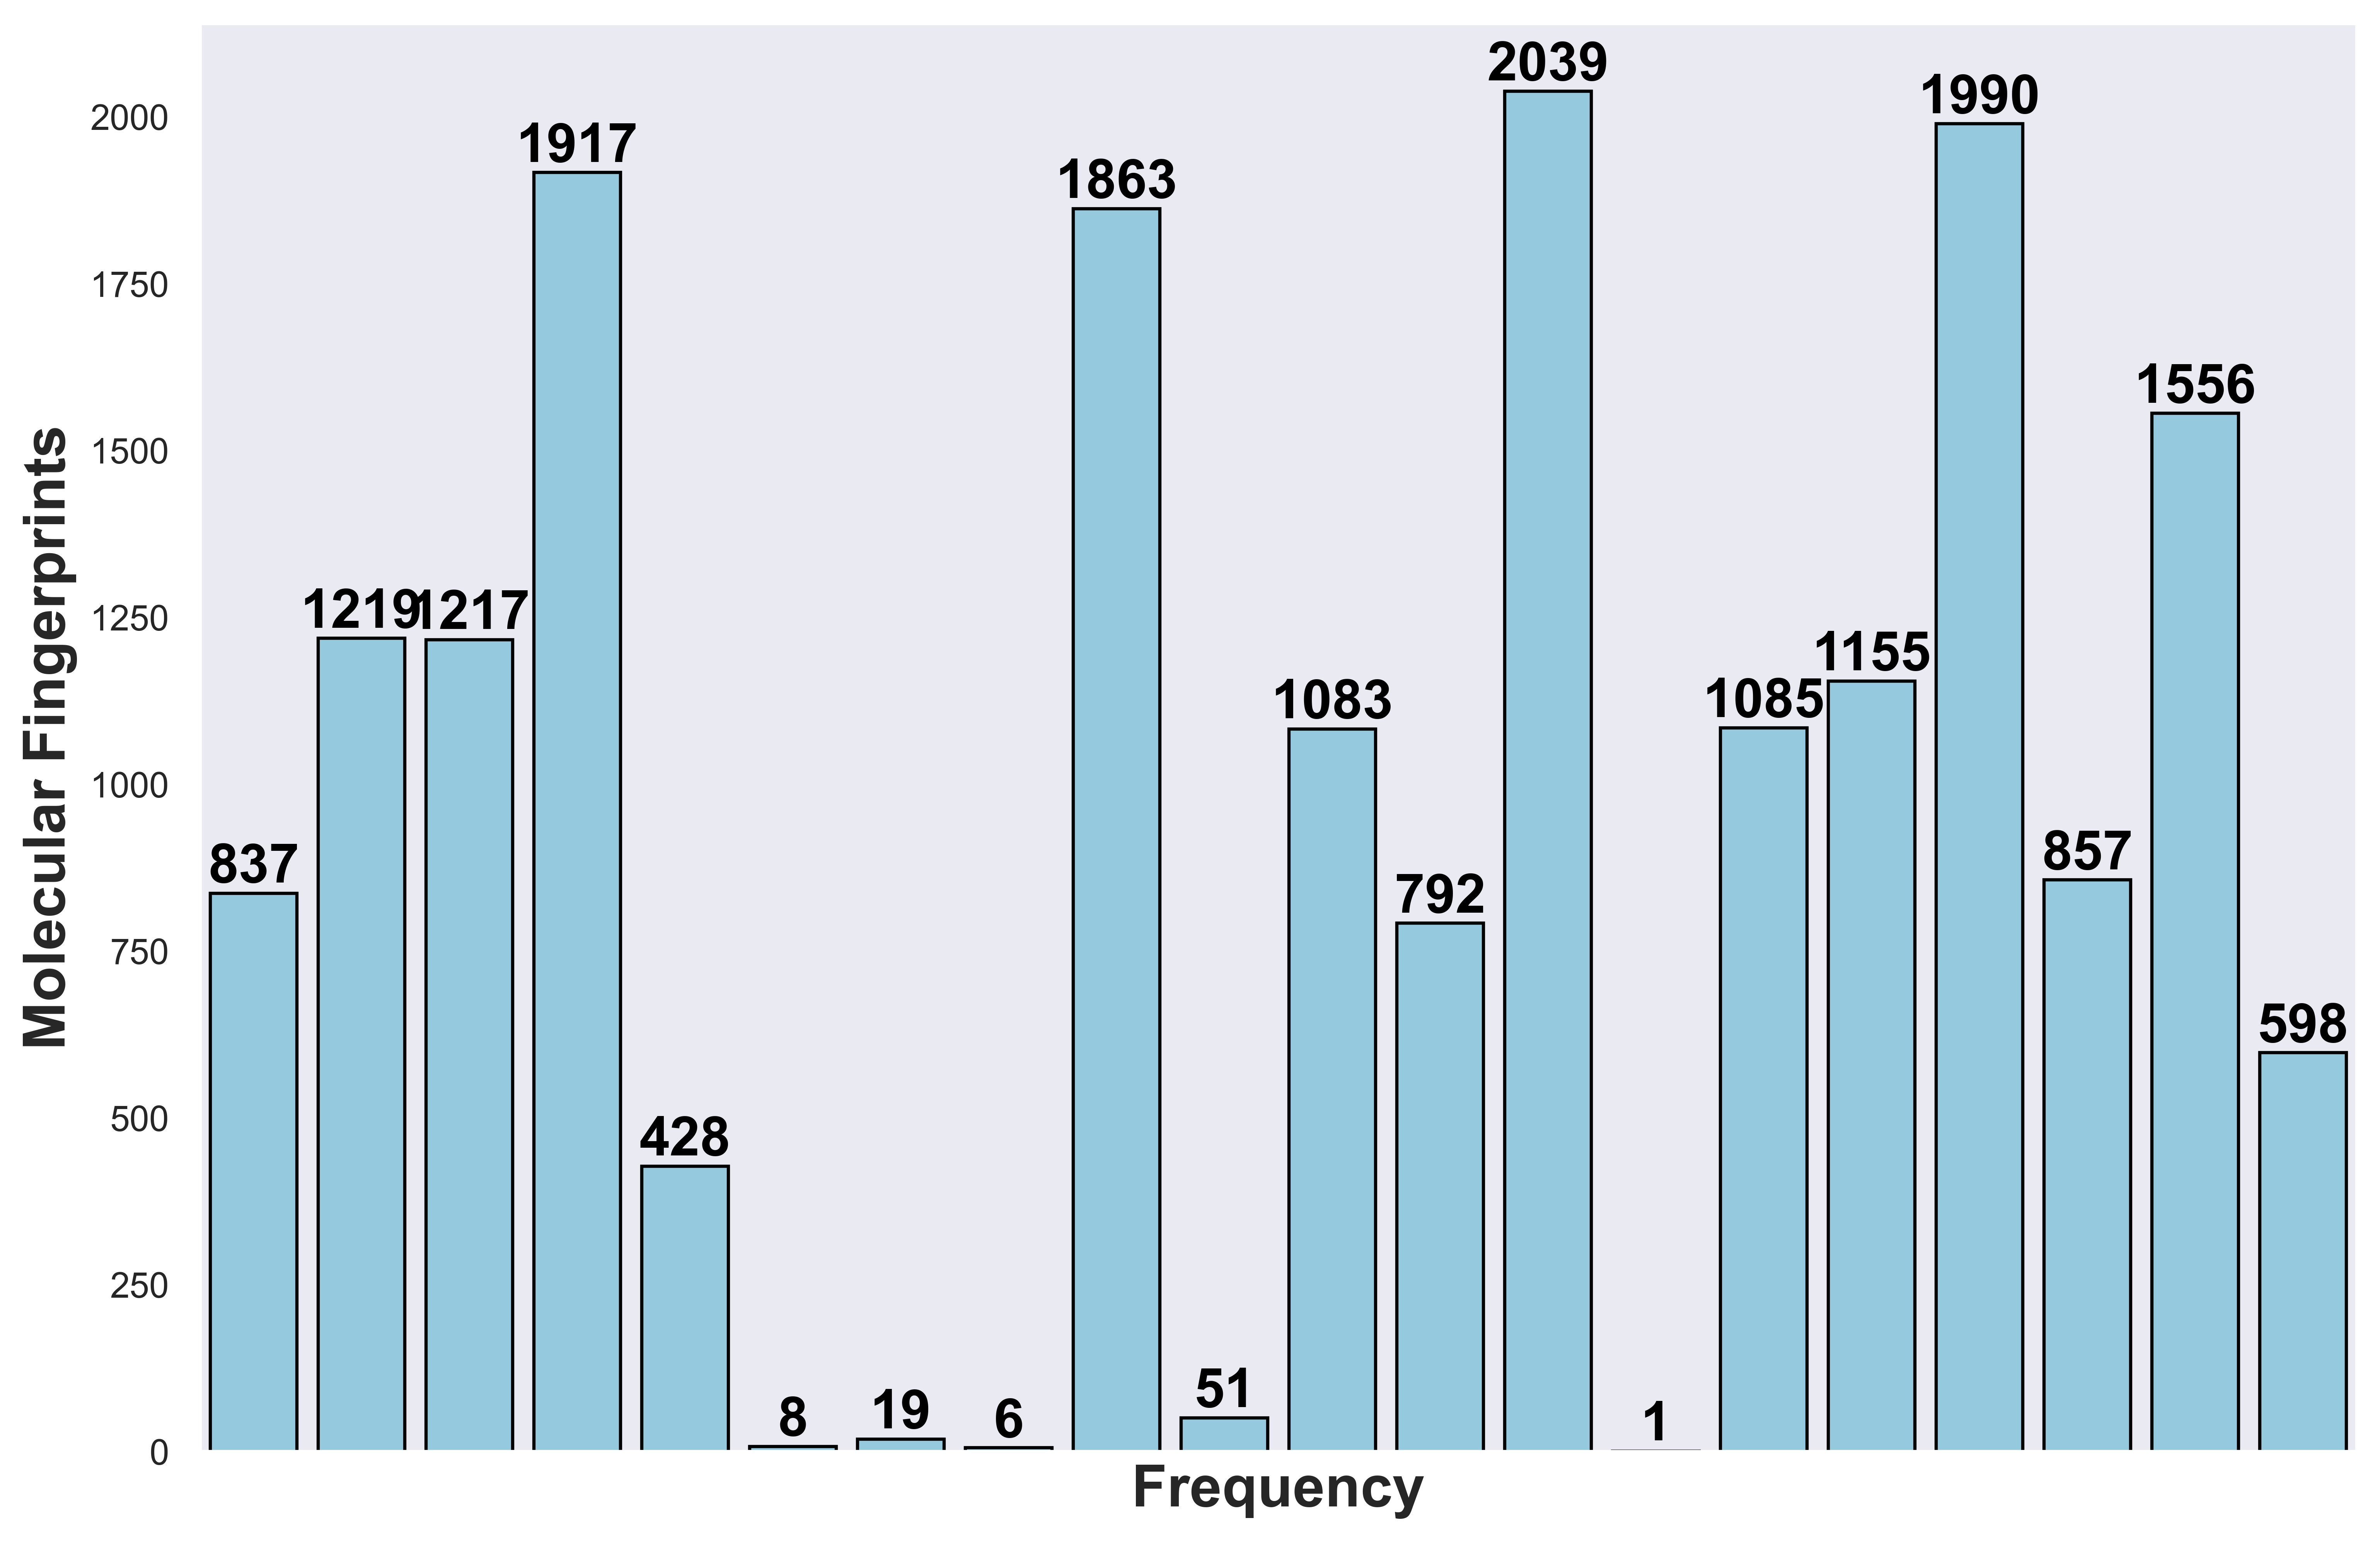
\includegraphics[width=0.8\textwidth]{bit_freq_chart.png}
		%\caption{Frequently Observed Bits in different Clusters}
		%\label{fig:most_common_bits}
	%\end{minipage}
%\end{figure}
%\FloatBarrier
\begin{figure}[h]
	\centering
	\begin{minipage}{\textwidth}
		\centering
		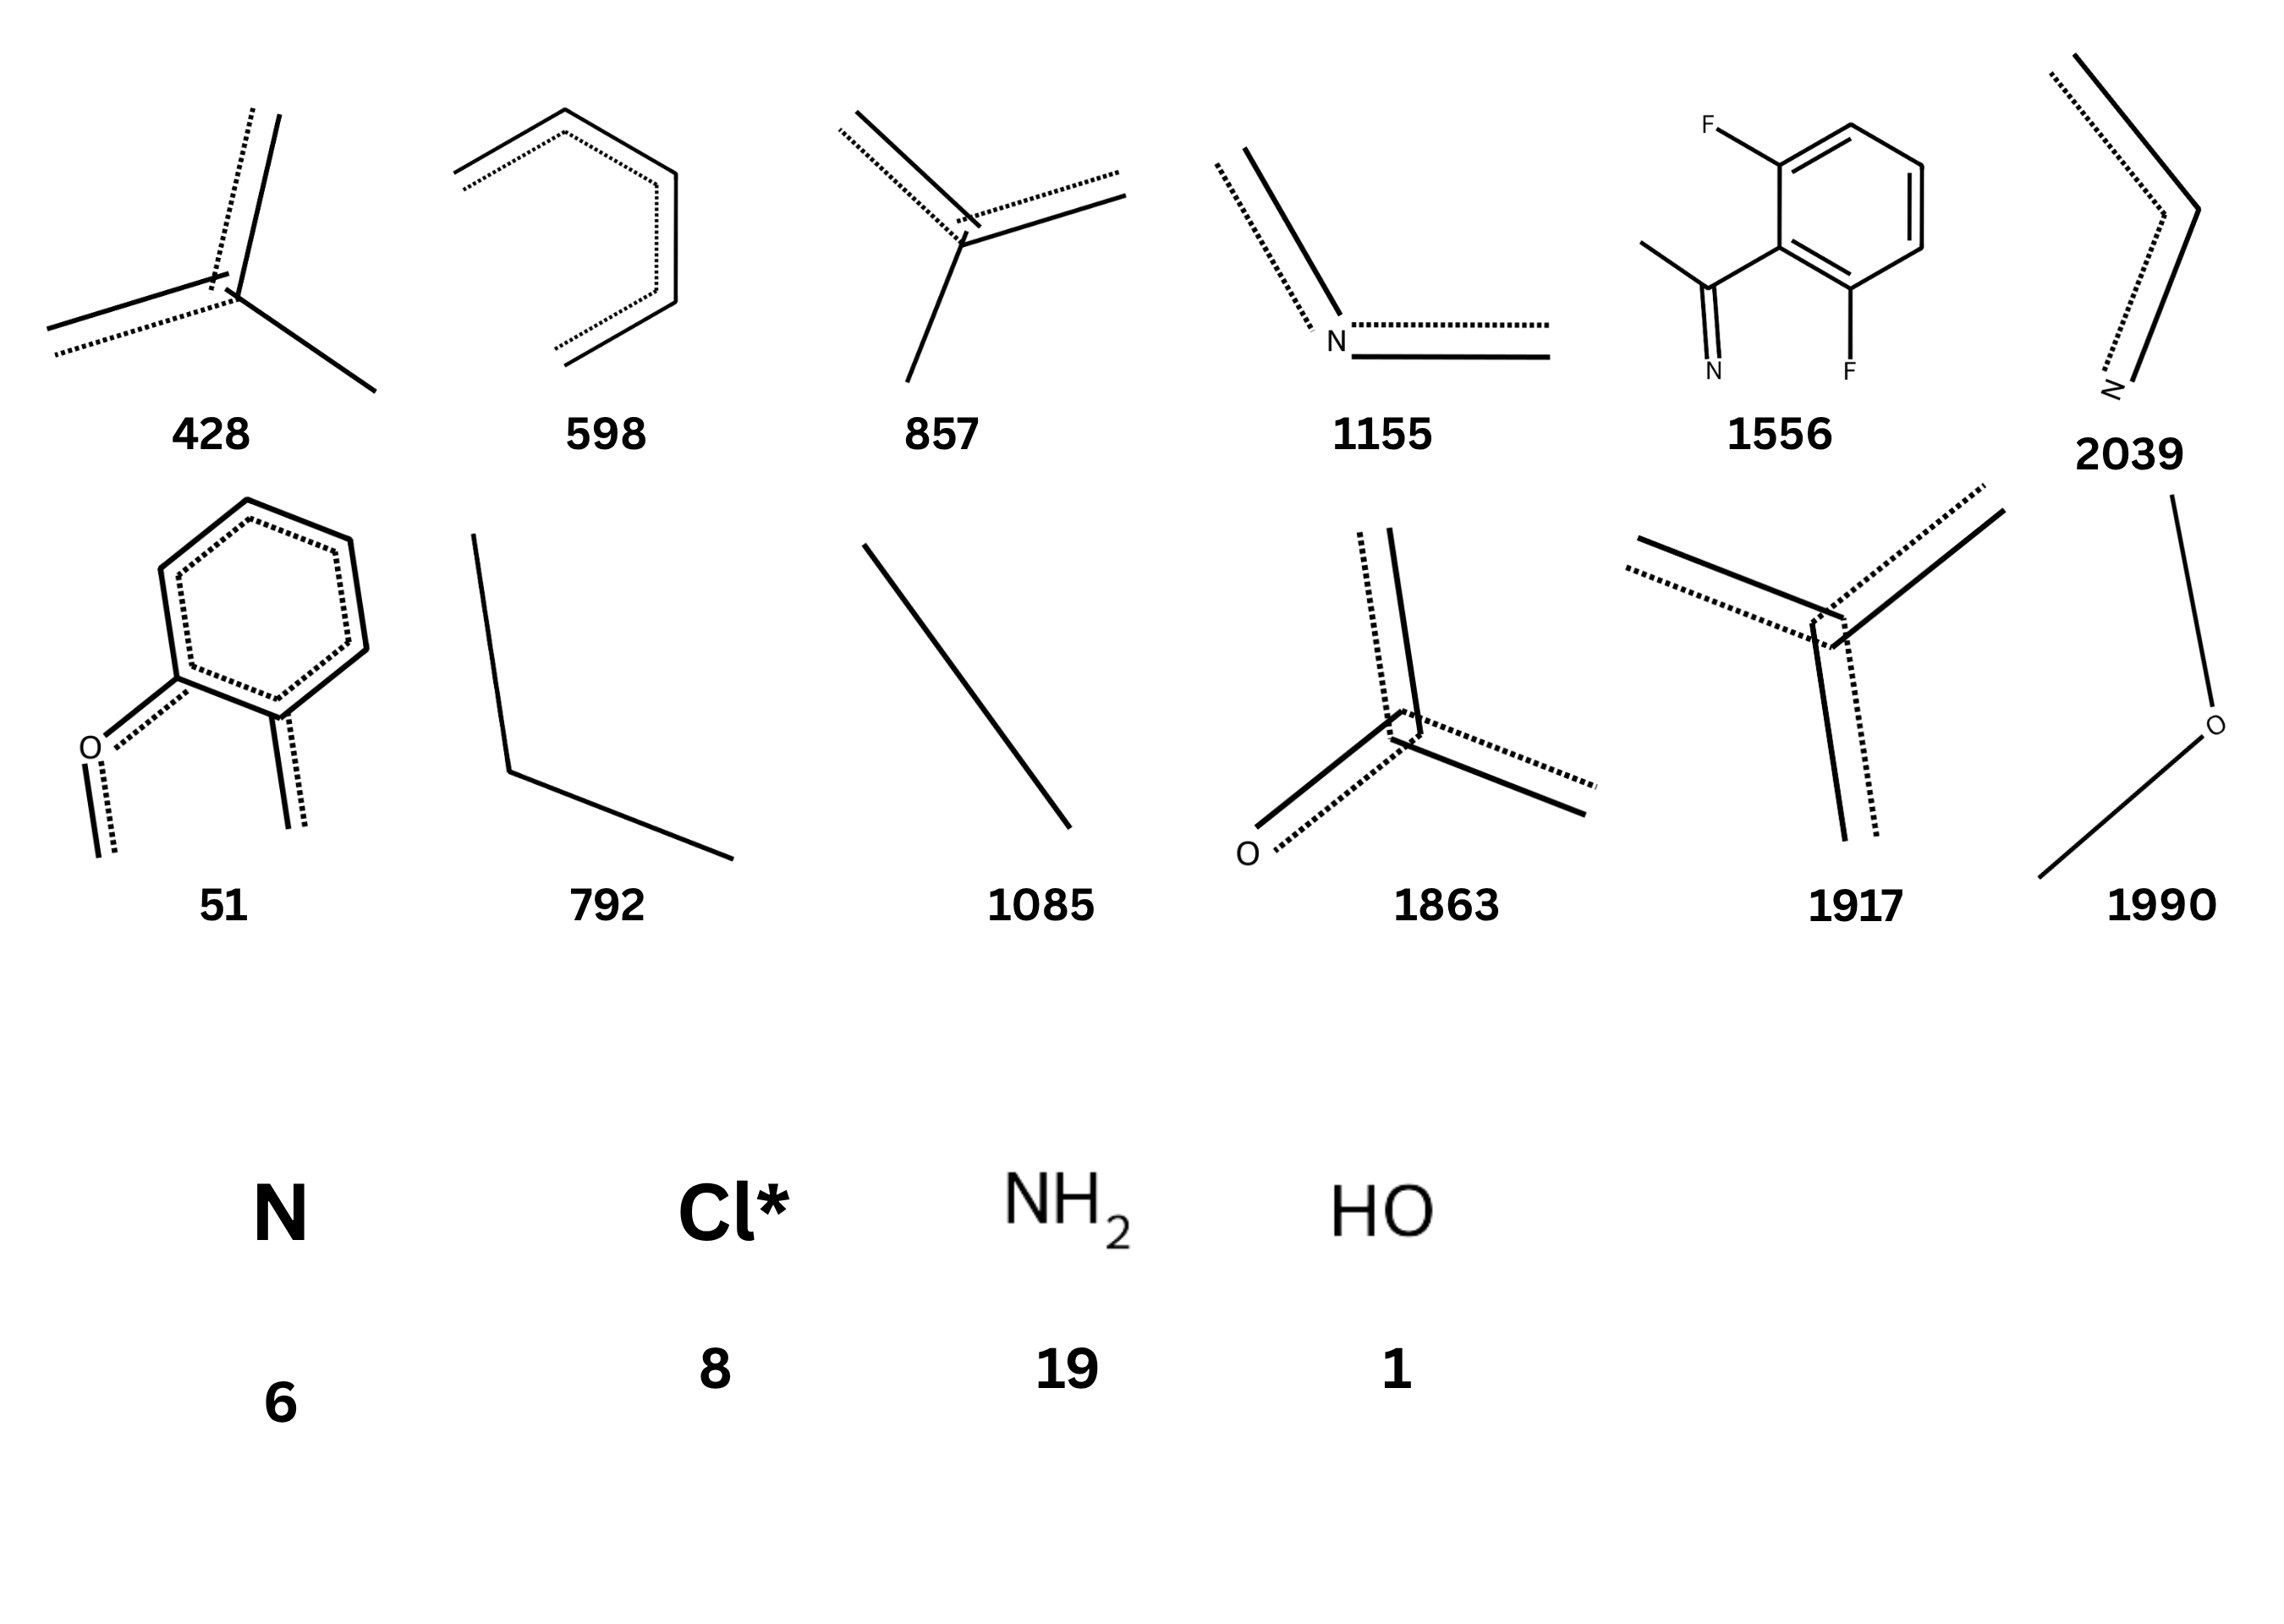
\includegraphics[width=0.8\textwidth]{mostcommonbitv2.png}
		\vspace{-0.3cm}
		
		\parbox{\textwidth}{\centering \footnotesize \textbf{*} Can be interpreted as other electronegative atoms/functional groups.}
		
		\vspace{0.3cm}
		\caption{Most common bits visualization:CSBC}
		\label{fig:mostcombits}
	\end{minipage}
\end{figure}
\FloatBarrier
\subsection*{CBC-ML and CSBC-ML Development}

\begin{table}[h]
	\centering
	\small
	\renewcommand{\arraystretch}{1.2}
\resizebox{\textwidth}{!}{%
	\begin{tabular}{p{3.5cm} p{1.5cm} c c c c c c c}
		\hline
		\textbf{QSAR-ML Model} & \textbf{Phase} & \textbf{Accuracy} & \textbf{Precision} & \textbf{Recall} & \textbf{F1 Score} & \textbf{Specificity} & \textbf{FNR} & \textbf{FPR} \\
		\hline
		CSBC-ML-Logit & Training & 0.7061 & 0.6985 & 0.7279 & 0.7129 & 0.6842 & 0.2721 & 0.3158 \\
		& Testing  & 0.7092 & 0.6976 & 0.7285 & 0.7127 & 0.6842 & 0.2721 & 0.3158 \\
		CBC-ML-Logit  & Training & 0.6328 & 0.6290 & 0.6519 & 0.6403 & 0.6136 & 0.3481 & 0.3864 \\
		& Testing  & 0.6214 & 0.6134 & 0.6366 & 0.6248 & 0.6136 & 0.3481 & 0.3864 \\
		CBC-ML-XGB    & Training & 0.7299 & 0.7344 & 0.7222 & 0.7283 & 0.7376 & 0.2778 & 0.2624 \\
		& Testing  & 0.7206 & 0.7143 & 0.7260 & 0.7201 & 0.7152 & 0.2740 & 0.2848 \\
		CSBC-ML-XGB   & Training & 0.9560 & 0.9347 & 0.9808 & 0.9572 & 0.9312 & 0.0192 & 0.0688 \\
		& Testing  & 0.9488 & 0.9240 & 0.9770 & 0.9498 & 0.9212 & 0.0230 & 0.0788 \\
		CSBC-ML-RF    & Training & 0.9562 & 0.9348 & 0.9812 & 0.9574 & 0.9312 & 0.0188 & 0.0688 \\
		& Testing  & 0.9484 & 0.9233 & 0.9770 & 0.9494 & 0.9204 & 0.0230 & 0.0796 \\
		CBC-ML-RF     & Training & 0.7300 & 0.7346 & 0.7222 & 0.7284 & 0.7378 & 0.2778 & 0.2622 \\
		& Testing  & 0.7206 & 0.7143 & 0.7260 & 0.7201 & 0.7152 & 0.2740 & 0.2848 \\
		CSBC-ML-SVM   & Training & 0.9476 & 0.9283 & 0.9704 & 0.9489 & 0.9247 & 0.0296 & 0.0753 \\
		& Testing  & 0.9435 & 0.9239 & 0.9655 & 0.9442 & 0.9220 & 0.0345 & 0.0780 \\
		CBC-ML-SVM    & Training & 0.7300 & 0.7346 & 0.7222 & 0.7284 & 0.7378 & 0.2778 & 0.2622 \\
		& Testing  & 0.7206 & 0.7143 & 0.7260 & 0.7201 & 0.7152 & 0.2740 & 0.2848 \\
		\hline
	\end{tabular}
}
	\caption{Combined training and testing performance metrics of CBC-ML and CSBC-ML Models}
	\label{tab:combined_metrics}
\end{table}

\begin{figure}[h] % 'h' places the figure approximately here
	\centering
	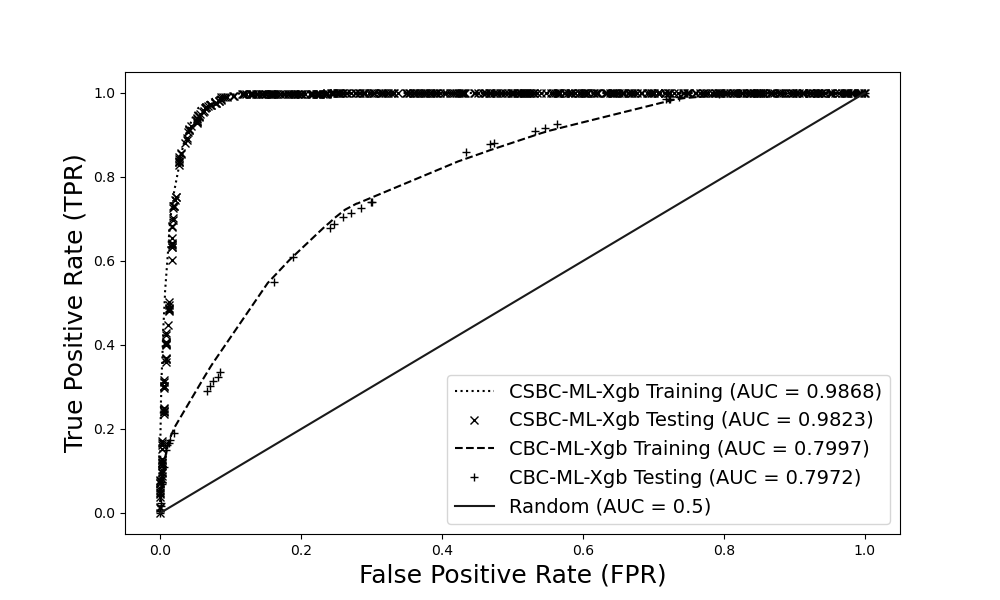
\includegraphics[width=0.8 \textwidth]{csbc_cbc_xgb.png} % Replace with your image filename
	\caption{Comparative summary of CSBC-ML-XGB and CBC-ML-XGB: ROC Curve}
	\label{fig:model_comparison_roc} % Optional: use \label for referencing
\end{figure}

\begin{figure}[h] % 'h' places the figure approximately here
	\centering
	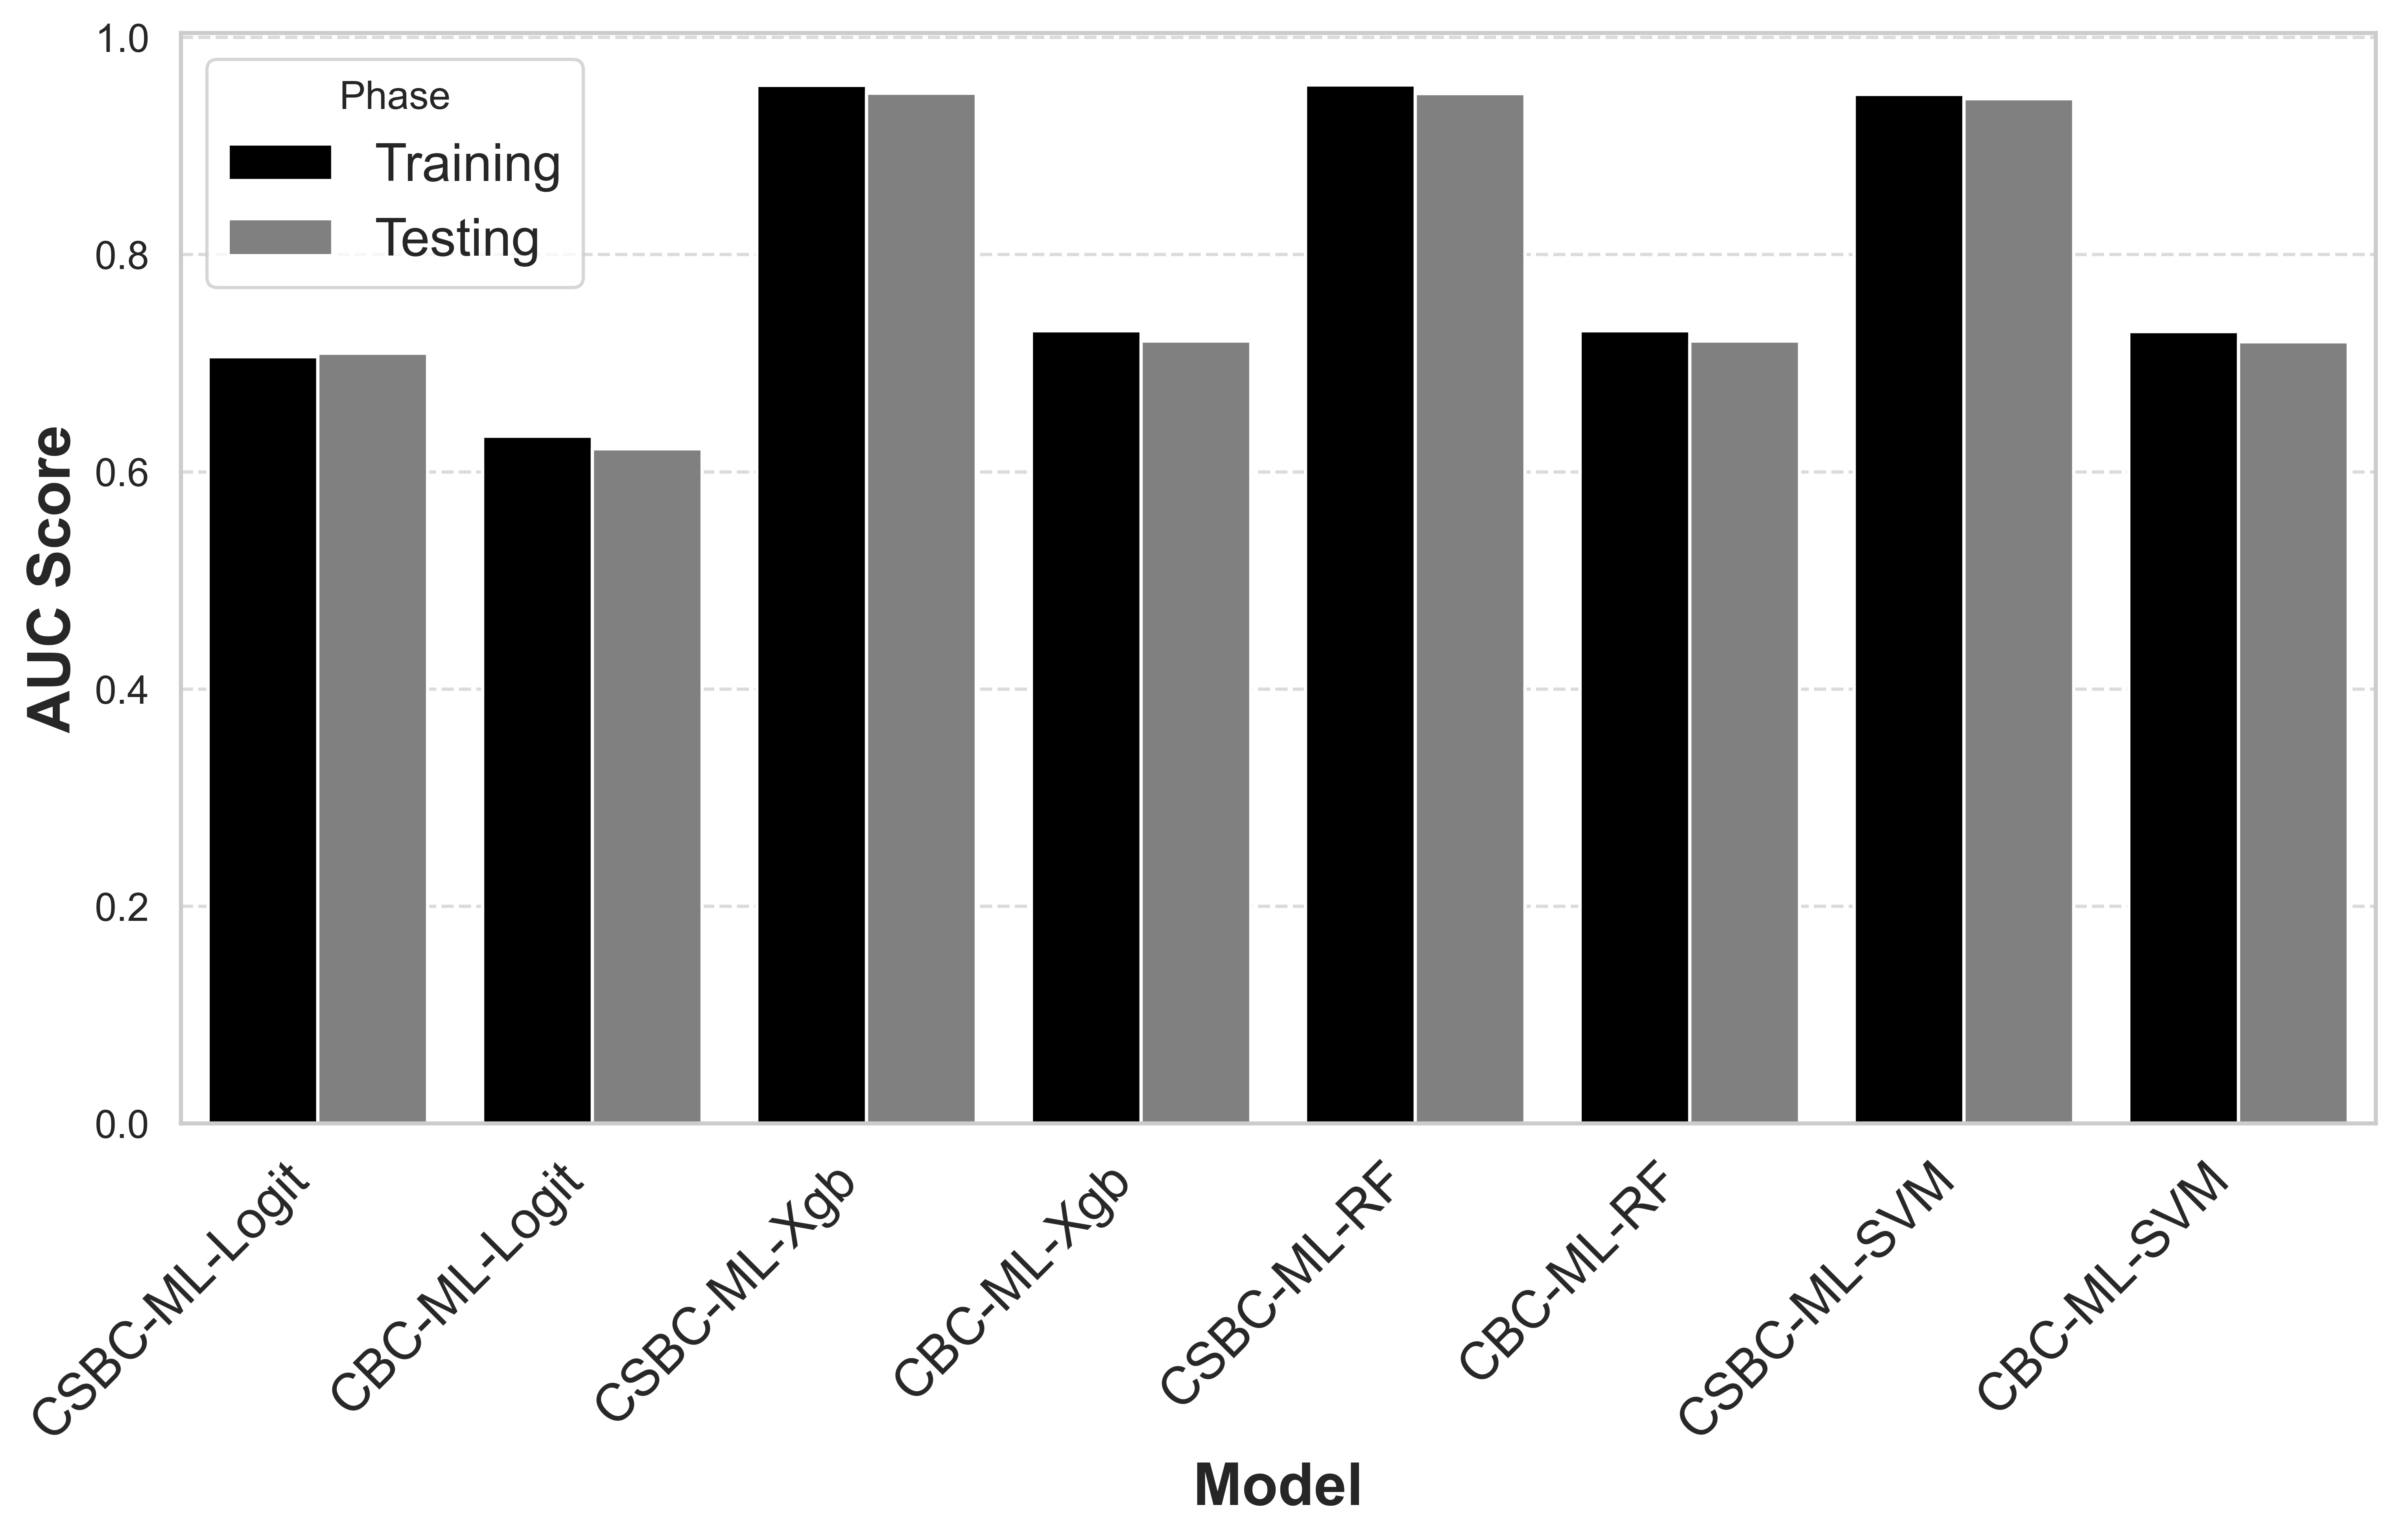
\includegraphics[scale=0.6]{auc_comparisonbw.png} % Replace with your image filename
	\caption{Comparative summary of CSBC-ML and CBC-ML: AUC Scores}
	\label{fig:model_comparison_auc} % Optional: use \label for referencing
\end{figure}

Logit models of CSBC produced an average of 70 \% in terms accuracy, recall, f1 and AUC score, together with FNR and FPR of 27 \% and 31 \% respectively. The same metrics for CBC logit models were found to be 63 \%, 34 \% and 38 \%, respectively (\autoref{tab:combined_metrics}). For XGB, RF AND SVM models, results revealed that CBC produced an average of 70\% for accuracy, recall, f1 and AUC score, 30 \% FNR and FPR while CSBC had an average of 94 \% in accuracy, 1 \% FNR and FPR, 98 \% recall, f1 and AUC score. CSBC models appeared to excellently classify activity against HCT-116, and it has a strong ability to generalize unknown data with minimal false predictions. On the other hand, CBC models have moderate predictive capacity and might suffer false predictions when unknown data increases. Overall, it was observed that CSBC models significantly outperforms CBC models in terms of confusion matrix parameters and AUC score. (\autoref{tab:combined_metrics}, \autoref{fig:model_comparison_auc}). The ROC curves showed that all the CBC-ML models suffered from over-fitting, whereas CSBC-ML models showed good fit even with unknown data. This suggests that CSBC-ML might be robust against increasing data set. \autoref{fig:model_comparison_roc} shows a sample comaparison of CSBC-ML and CBC-ML models. 



	
	\section*{Discussions}
	\subsection*{Structural Analysis: Generation of MFP }

%\subsubsection*{a. Structure Subtraction and Counting}

%The main difference between CBC and CSBC method is that the latter uses structure subtraction operation to segregate the bits base on its significance. Structure subtraction is a procedure that is part of CSBC method that is devised by the researchers to extract the structural pattern dependence on position and neighbors. To CSBC method work, the following assumptions must be fulfilled; a) all of the compounds must undergo fragmentation via MFA to generate MP's; b) generated MP's was converted to matrix (1x2048); c) a neutral point must be assign, wherein, in this region the activity of compounds against HCT-116 is close to 0; d) difference in MP's of compounds located in neutral point vs the other region were considered to be significant bits; e) after structure subtraction, it will yield to formation of new MP's, the 1's, -1's and 0's were considered to be significant and non-significant bits(\autoref{fig:subtraction}. To account the positions and neighbors, the new MP's produced by structure subtraction were recompiled into clusters of HI-VLI, MI-VLI, LI-VLI, and NI-VLI. The produced clusters essentially contains the information about what are the unique bits found in subtracting the neutral point to the groups of compound with high and low bioactivity. For the case of HI-VLI, it is expected that the matrix elements equivalent to 1 are the unique positive bits (molecular fingerprints) that is responsible for the high bioactivity of the said compound, while the 0's and -1's are the non-significant and negative bits. The same assumption were used for MI-VLI, and LI-VLI, however, for NI-VLI, since these compounds have negative bioactivity the definition of 1's and -1's were inverted. Given that assumptions to be true, the researchers hypothesized that, if the bits have positional and neighbor dependency, therefore, they must be repeatedly observed across the clusters. To prove this hypothesis, the researchers try to find whether the top bits from HI-VLI were present in MI-VLI, LI-VLI, and NI-VLI. The results shows that the top bits from HI-VLI which are 1, 6, 8, 19, 51, 428, 598, 792, 857, 1085, 1155, 1556, 1863, 1917, 2039 and 1990, were also the top bits in MI-VLI, LI-VLI and NI-VLI. Therefore, these bits has the characteristics to positively and negatively affect the compounds bioactivity, which can only be attributed to their position and to the types of neighbor they have. 
%\vspace{-0.7cm}
\begin{figure}[h] % 'h' places the figure approximately here
	\centering
	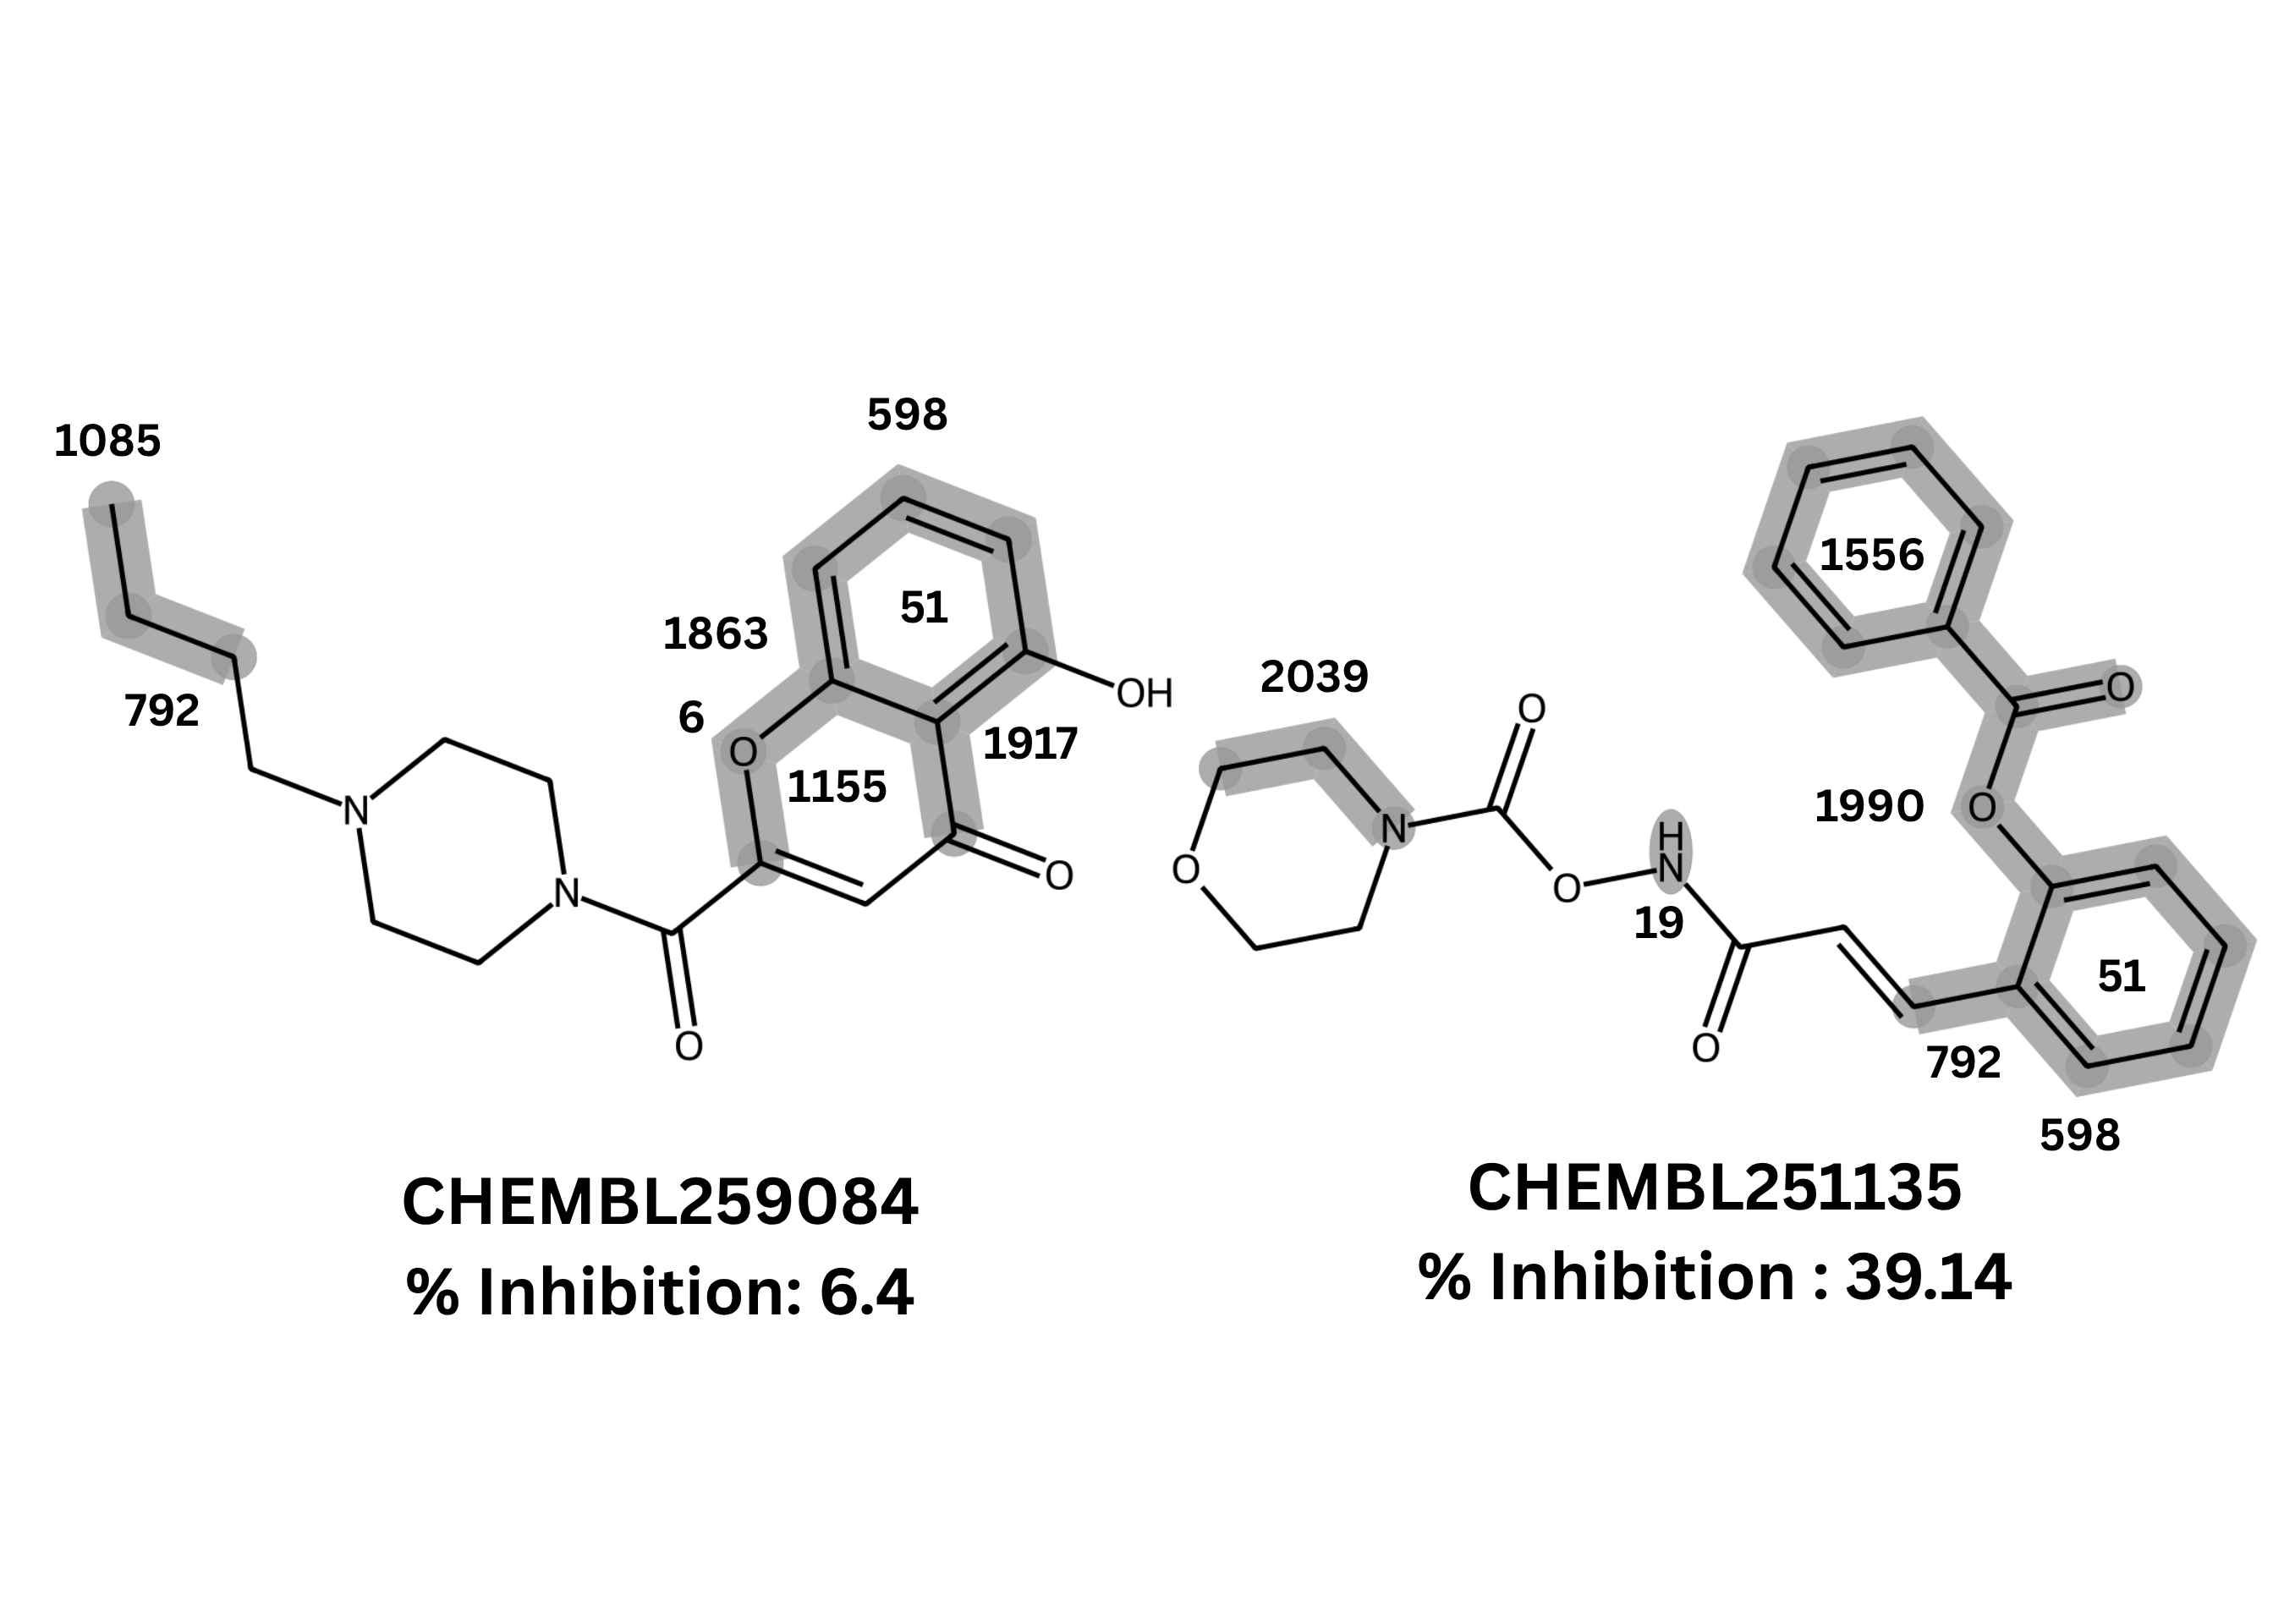
\includegraphics[width=0.8\textwidth]{6_4_vs_39_14_bits_visualization_bw.png} % Replace with your image filename
	\vspace{-0.7cm}
	\caption{Bits Detection of CSBC-ML:SAMPLE 1}
	\label{fig:bit_visualization_643914} % Optional: use \label for referencing
\end{figure}

\subsubsection*{a. Structural Analysis of Bits: Positions and Neighbors}

\begin{figure}[h] % 'h' places the figure approximately here
	\centering
	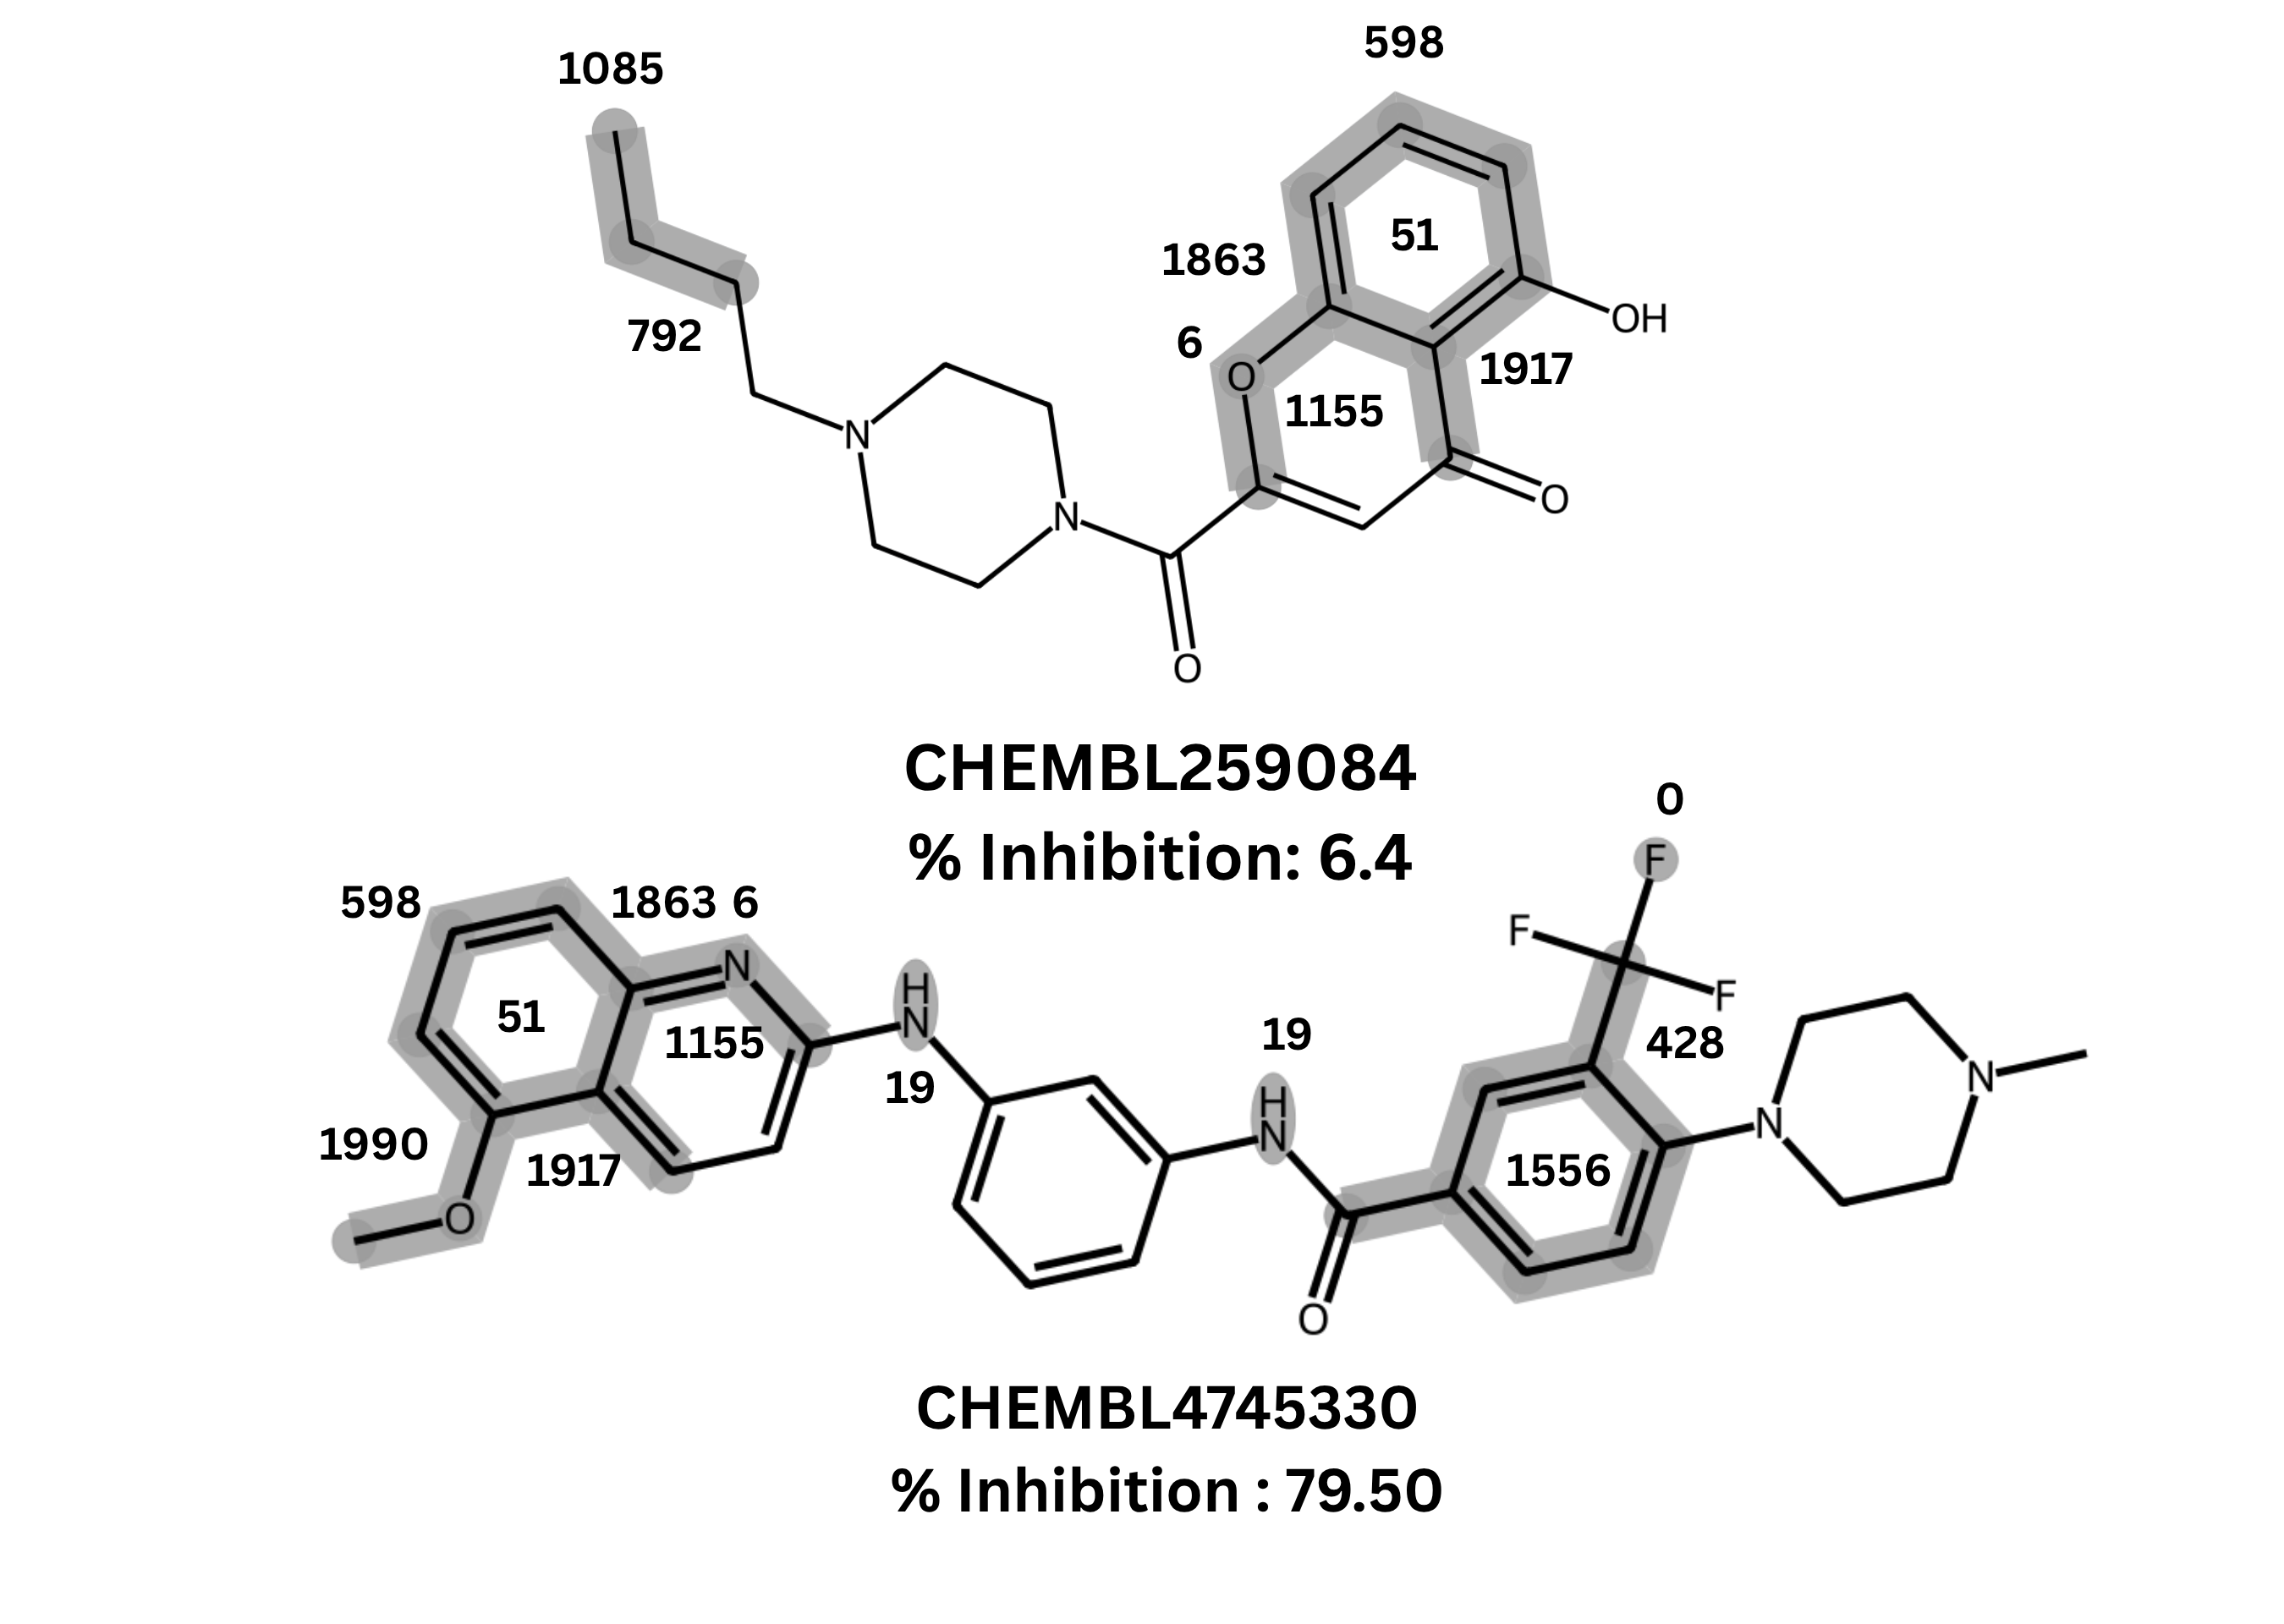
\includegraphics[width=0.7\textwidth]{79_5vs_6_4_bit_visualization_bw.png} % Replace with your image filename
	\caption{Bits Detection of CSBC-ML:SAMPLE 2}
	\vspace{-0.3cm}
	\label{fig:bit_visualization_7939} % Optional: use \label for referencing
\end{figure}

\begin{figure}[h] % 'h' places the figure approximately here
	\centering
	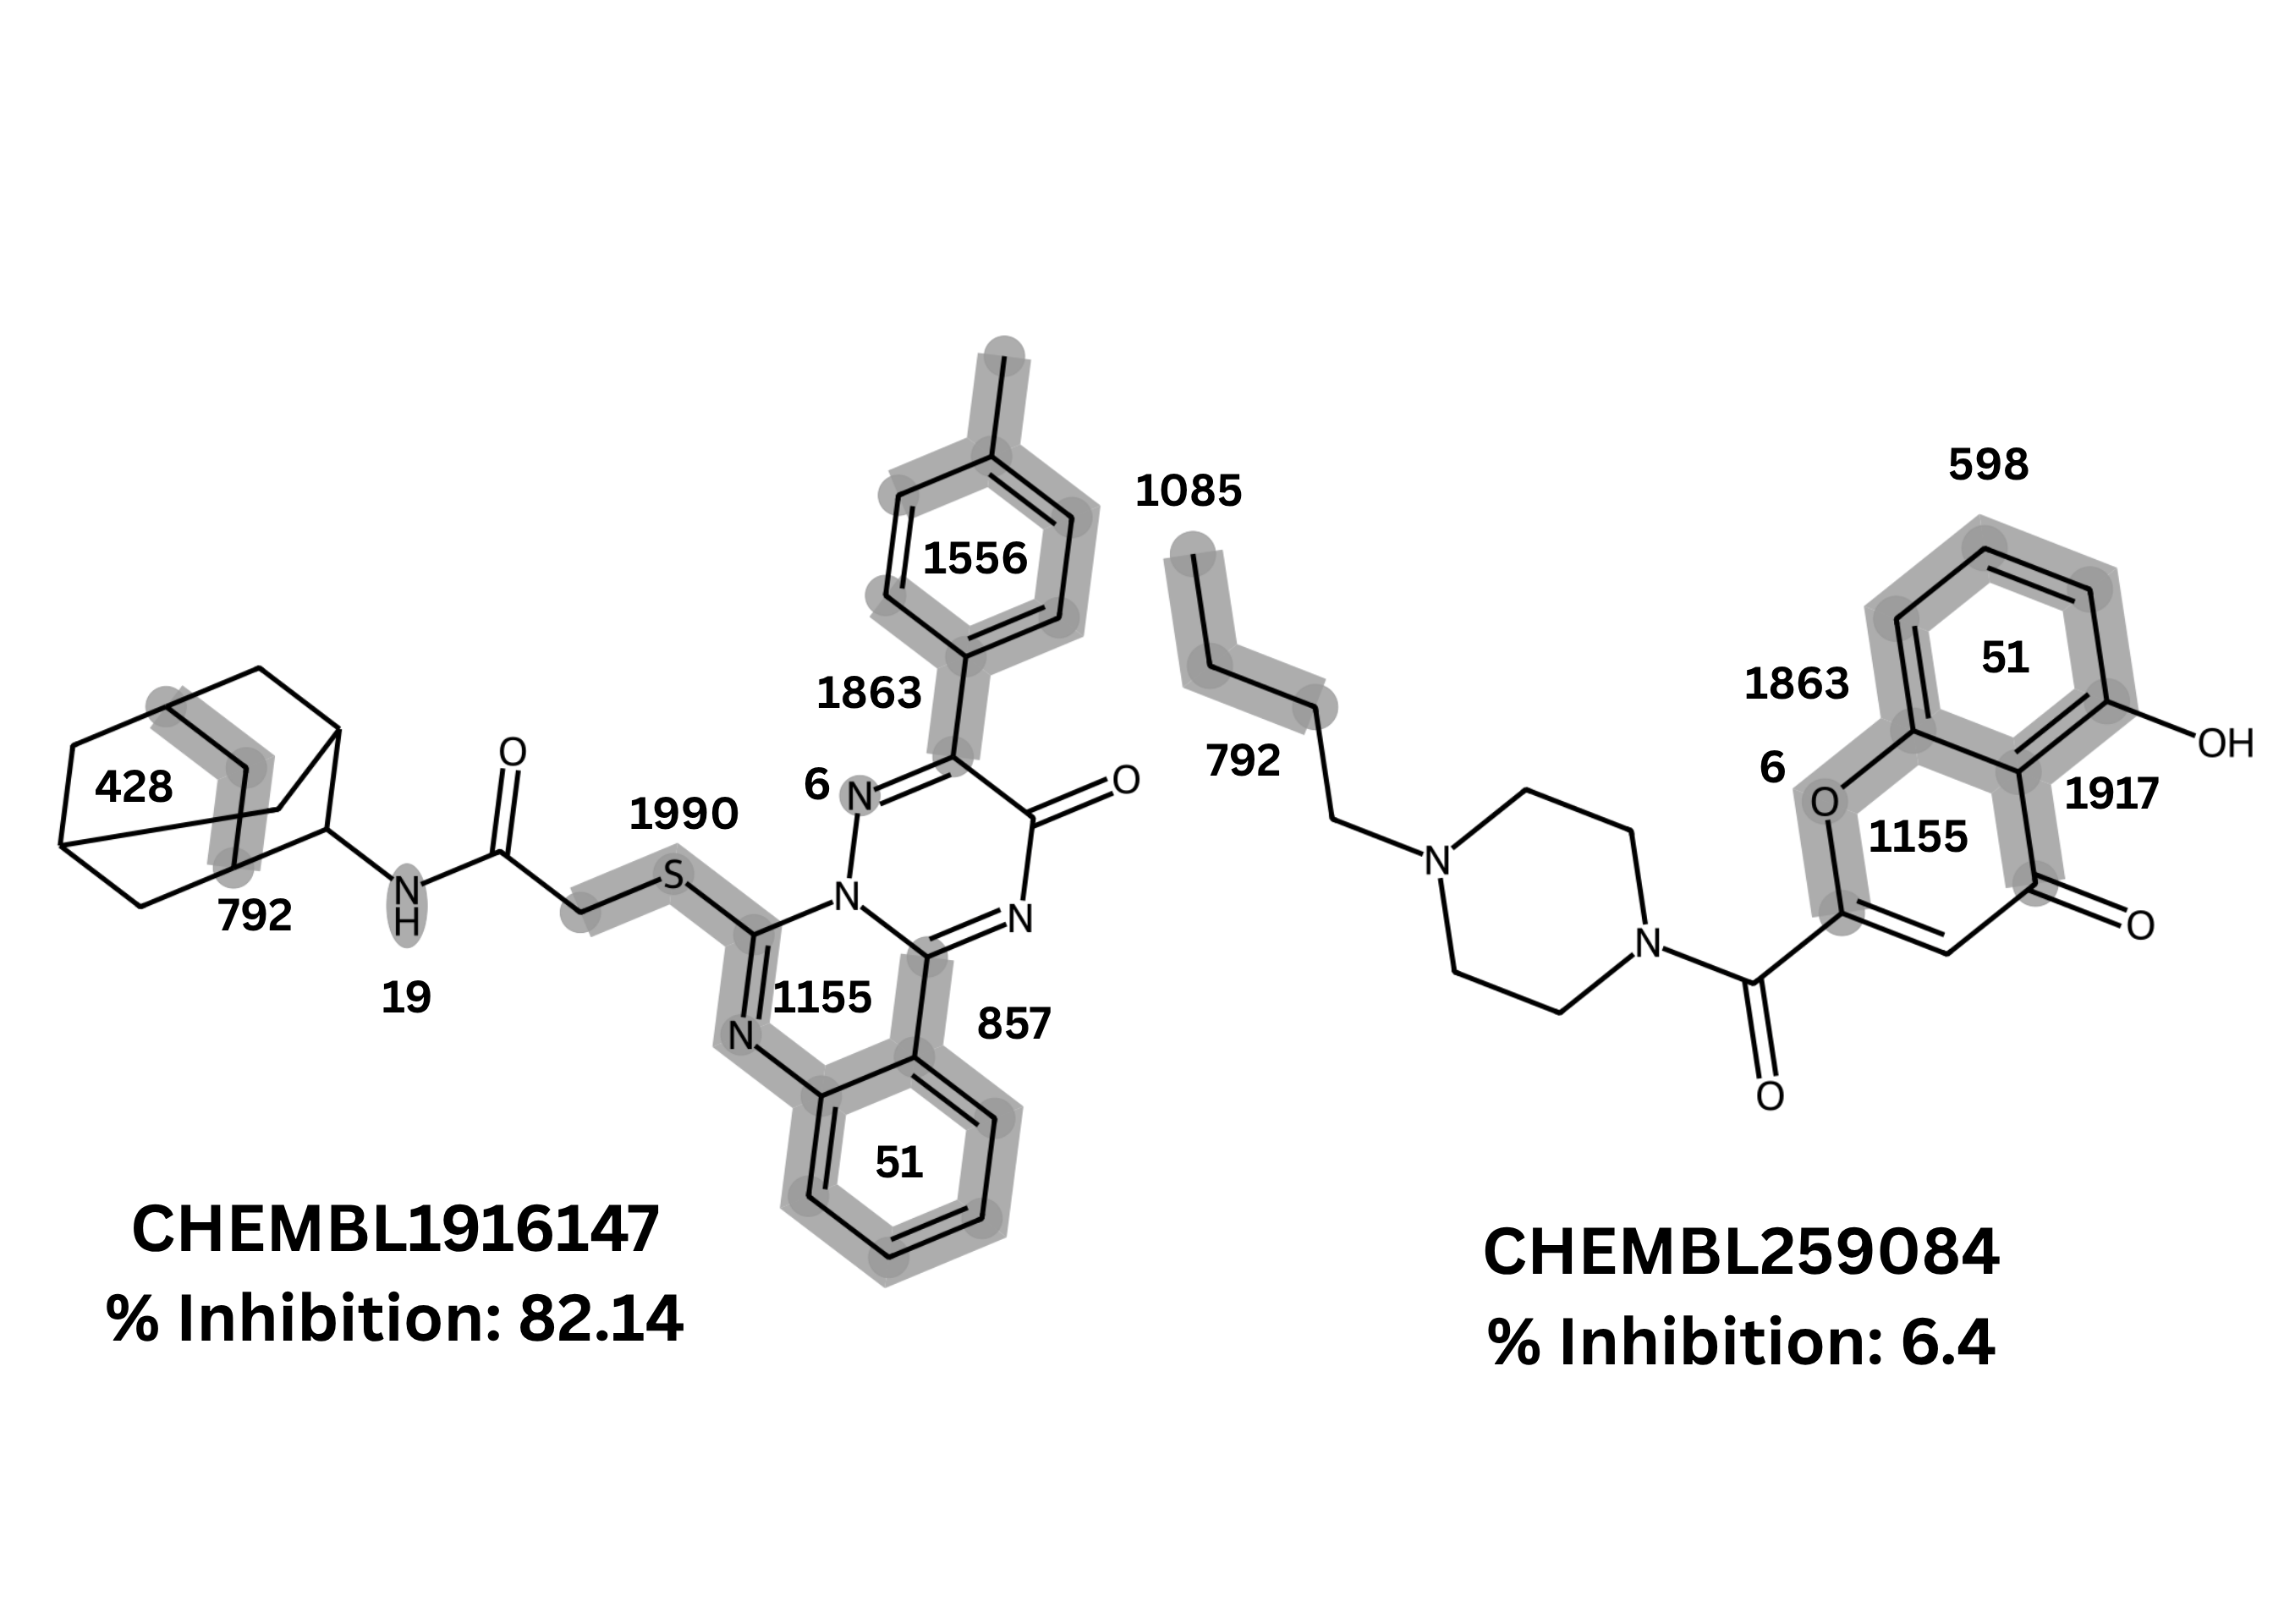
\includegraphics[width=0.7\textwidth]{82_14_vs_6_4_bits_visualization_bw.png} % Replace with your image filename
	\caption{Bits Detection of CSBC-ML:SAMPLE 3}
	\vspace{-0.3cm}
	\label{fig:bit_visualization_8264} % Optional: use \label for referencing
\end{figure}

\begin{figure}[htbp!] % 'h' places the figure approximately here
	\centering
	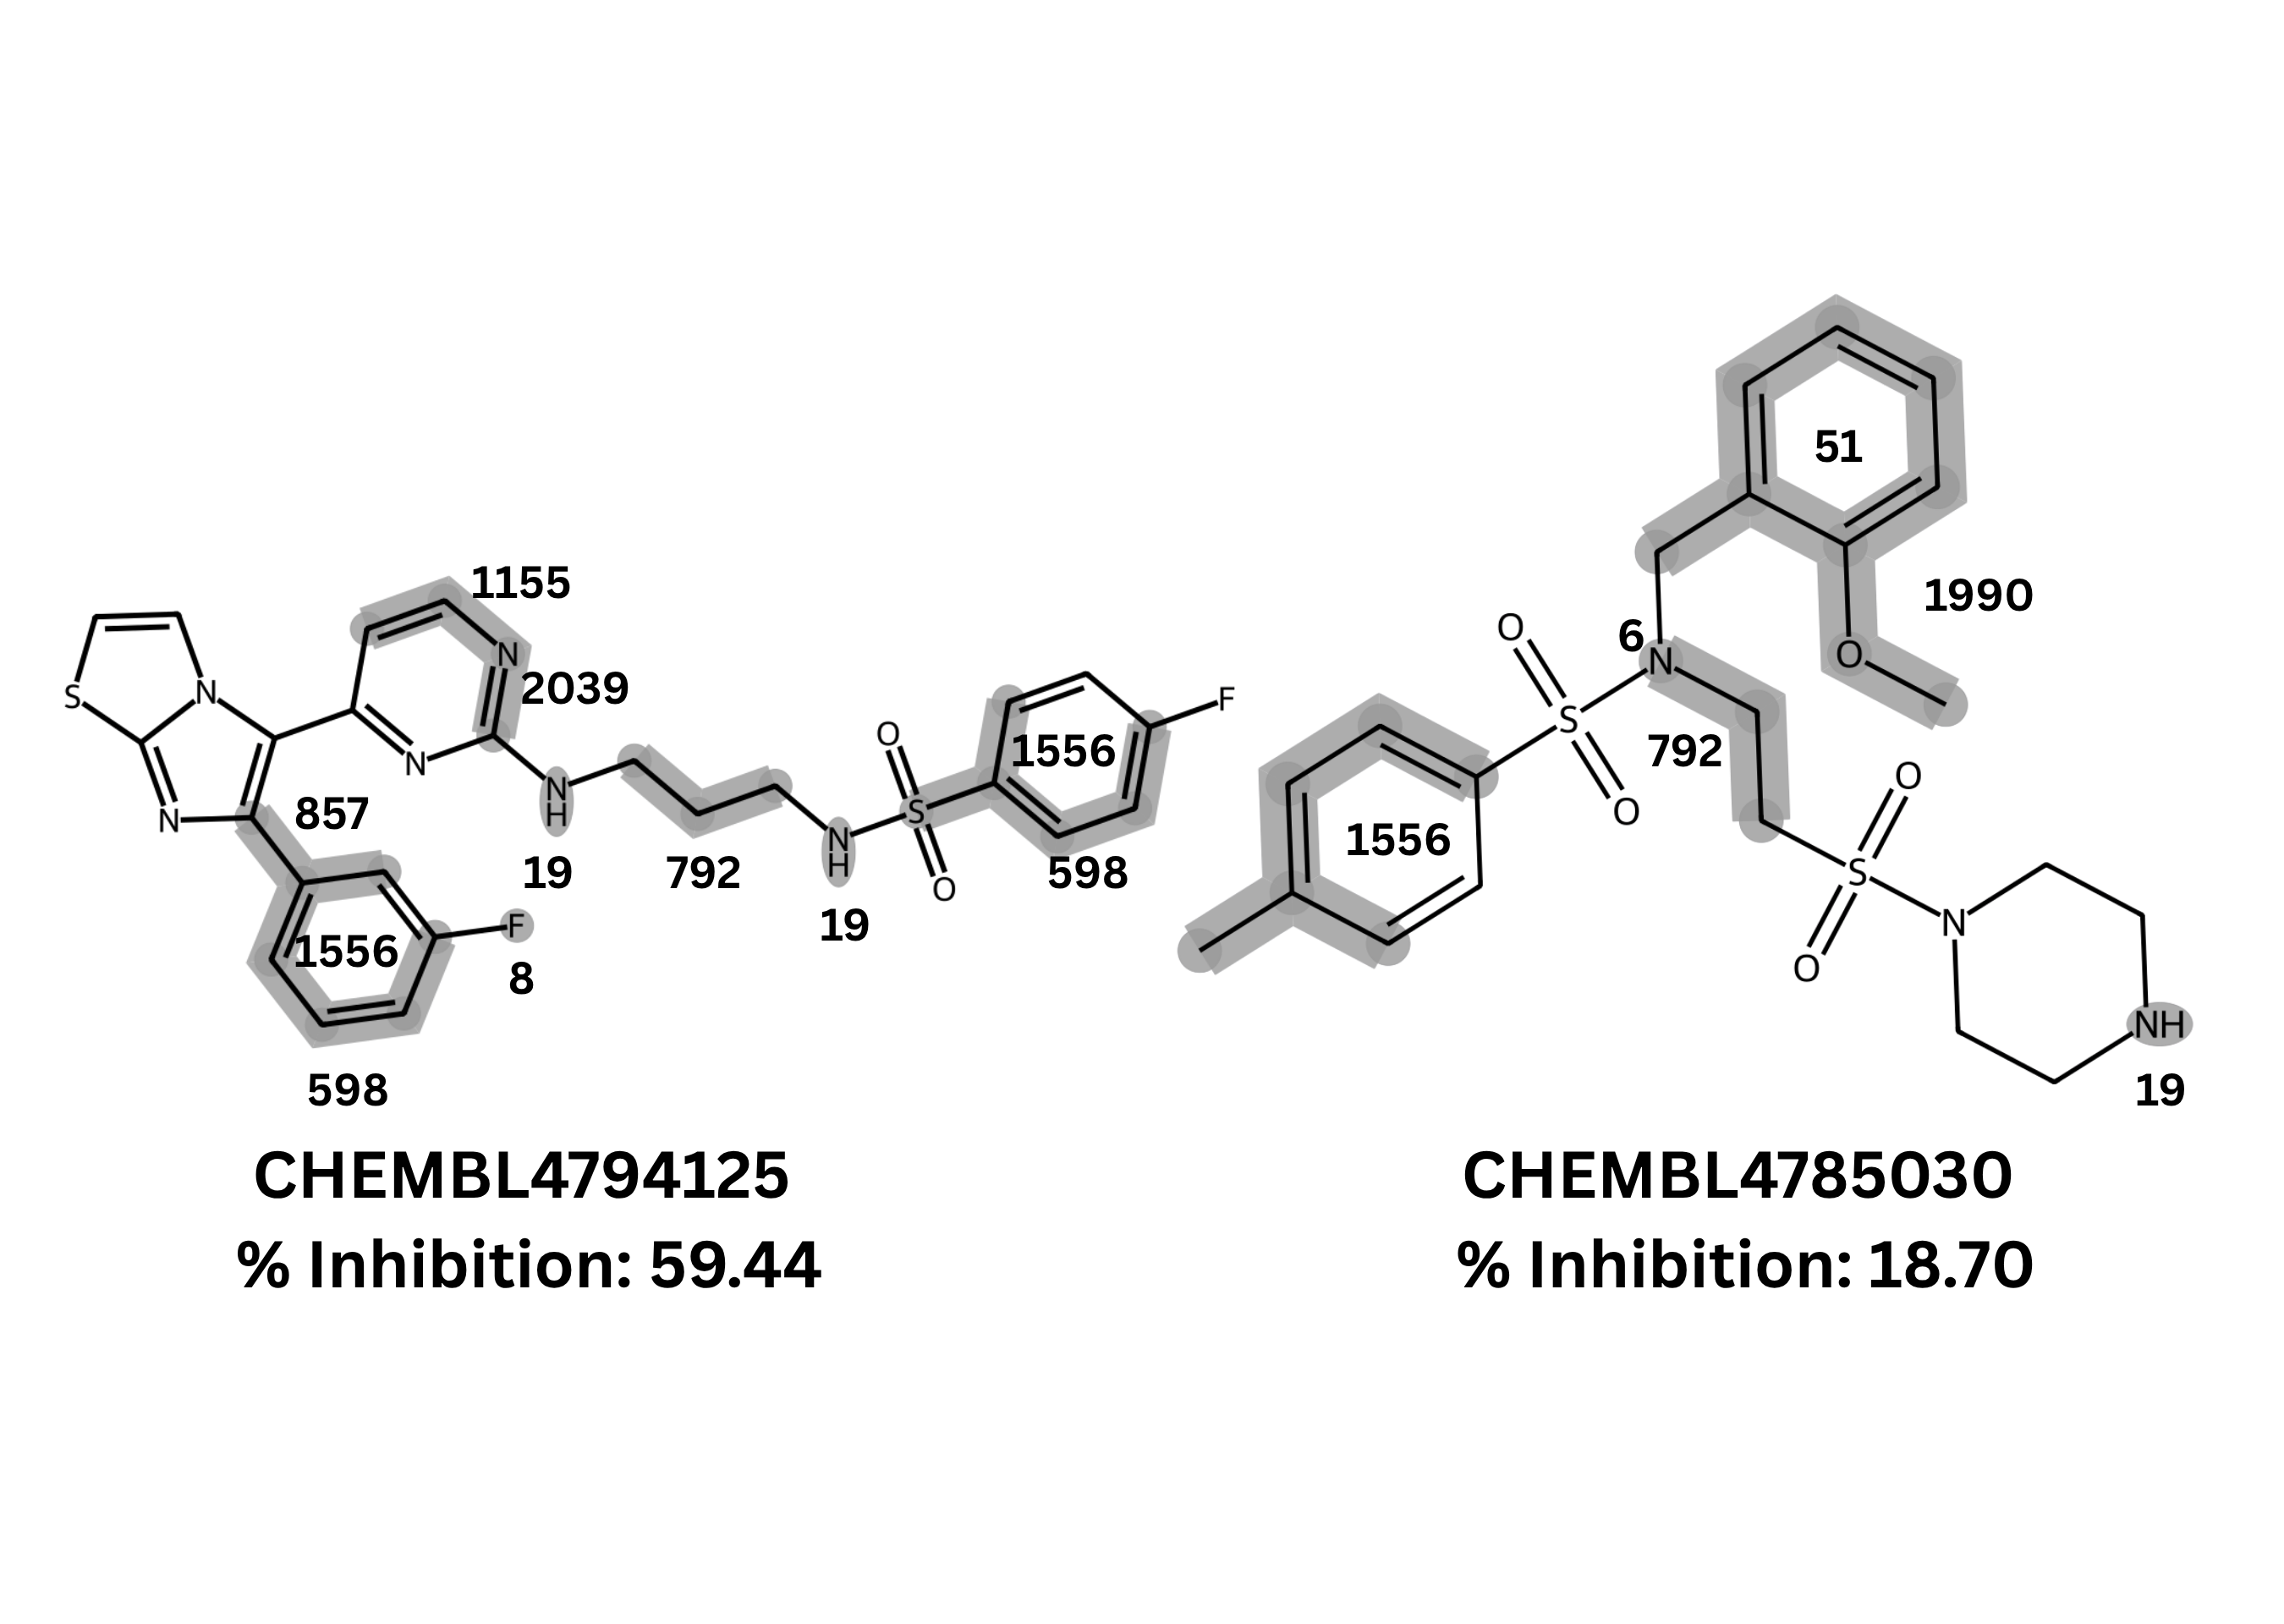
\includegraphics[width=0.8\textwidth]{3_403_mol_inhibition.png} % Replace with your image filename
	\caption{Bits Detection of CSBC-ML:SAMPLE 4}
	\vspace{-0.3cm}
	\label{fig:bit_visualization_5918} % Optional: use \label for referencing
\end{figure}

To validate bits positional and neighbor dependency, random molecules from the sample data set were taken, and subsequently fed to the CSBC-ML models (XGB, RF, SVM) for bit presence determination. However, this time the results were extracted as 2D image structure (png) file. \autoref{fig:bit_visualization_643914} - \ref{fig:bit_visualization_8264} shows some example of generated png files with bits of interest highlighted in grey. The figures show how the MLA perceived 2D structural queries during the training and testing periods. Inserted features (bits from CSBC) are highlighted and the irrelevant ones are not. It was observed that molecule CHEMBL259084 has an attributes of positive bits which are 1085, 792, 1863, 1155, 1917, 6, 51, and 598  but, its \% Inhibition against HCT-116 was only 6.4. On the other hand, CHEMBL251135 has also positive bits 2039, 19, 792, 598, 51, 1990, 1556, and its \% Inhibition was 39.14. Comparing the two molecules, the following can be observed: a) both of them have positive bits; b) they have common bits of 792, 51, 598; and c) the bioactivity of two molecules is significantly different. These observations can be explained by looking closely at their common bits. For instance in CHEMBL259084: bit 51 was positioned upward and close to bits 1863, 115 and 1917; bit 792 was situated far away from 51 and 598, close to 1085. On the other hand in CHEMBL251135, bit 51 was positioned downward and  close to 792, 598, 1990 and 1556 (\autoref{fig:bit_visualization_643914}). Another example is CHEMBL4745330,  %bits of 0, 6, 19, 51, 428, 598, 1155, 1556, 1863, 1917, and  1990,
comparing it to CHEMBL259084 they have common bits of 51, 598, 19, 1155, 1863, 1917, and 6 which are located at different positions but with almost the same neighbors --- only bit 1990 and 6 were added to it. (\autoref{fig:bit_visualization_7939}). These observations extends to other molecules such as CHEMBL1916147 (\% Inhibition 82.14) wherein bit 51 is positioned besides 857,1155, while bit 6 is near 1863, 1990, and 1156. In CHEMBL259084 they are positioned and neighbored differently (\autoref{fig:bit_visualization_8264}). These kind of observations were constantly observed throughout the randomized samples ---  \autoref{fig:bit_visualization_5918} shows the other subset of molecules. It is now apparent that the consolidation of similarities in position and structural neighborhood of bits from the cluster subtraction in CSBC were supported by observations on several structures that were visually inspected. From these results it can be drawn that qualitative structural analysis offers the visualization on the bits position and neighbor dependency, and that the results seems to validate all of the assumptions on significant bits dependency in position and neighbor. Furthermore, this might explain the compatibility of CSBC with XGB, RF and SVM models.
 
%Observing the structure of their common bits, 51 is positioned closed to bit 1863, 1155 and 1917 on an upward manner, bit 792 is situated far away from 51 and 598 but close to 1085 in CHEMBL259084, whereas, on CHEMBL251135, 51 is closed to 792, 598, 1990,1556, and protrude downward(\autoref{fig:bit_visualization_643914}). For other cases, CHEMBL4860630, has bits of 19, 1556, 1863, 1155, 1917, 2039, 1, 598 and 8, comparing it to CHEMBL251135 their common bits (598,19,1556,2039) were located at different positions and neighbors(\autoref{fig:bit_visualization_7939}). This extends to other molecules such as CHEMBL1916147 (\% Inhibition 82.14) wherein bit 51 is positioned besides 857,1155, while bit 6 is near 1863, 1990, and 1156 whereas in CHEMBL259084 they are positioned and neighbored differently (\autoref{fig:bit_visualization_8264}). Same kind of observations were seen throughout the randomized samples, hence, researchers conclude the following: a) qualitative structural analysis confirms and explains bits positional and neighbor dependency; b) the observation generated from it validates all of the assumptions on its compatibility as a feature on Xgb, RF and SVM models, wherein it is assumed that it will be forced to recognized the bits positional and neighbor dependency which in effect correcting its predictions; and c) the excellent performances of the CSBC-ML models is attributed to the correct selection of features. 
    

\subsubsection*{b. QSAR-ML Position and Neighbor Effects Rationalization}
CBC only relies on the presence and absence of MFP, and expects a linear relationship between the structure and target activity. Since it does not incorporate position and neighbor information, it was shown to result misclassifications. On the other hand, CSBC features were extracted and selected based on commonality across a given set of molecules. The top most common bits from CSBC are the collection of structures that are present in both active and inactive molecules, allowing non-linear mathematicals model combined to it implicitly accounts for the position and neighbors of the MFP. 

Among all of the mathematical models used in this study, logit performs the least in terms of confusion matrix parameters, AUC and ROC. This observation remains even if it is combined with CSBC features, and this can be attributed to the linearity of Logit, resulting to its inability to perceive position and neighbor differences of the bits. Therefore, it is difficult for the model to change its feature weights during the training and testing period, resulting to poor performance when compared to the other mathematical models. On the other hand, XGB, RF and SVM are mathematical models that have a self-correcting features. For XGB, the predictions are corrected by a log loss function, consisting of gradient and hessian functions that lets the model know far the predictions are from true values, which subsequently adjusts the step sized based on confidence in correction (\ref{eq:gradienthessian}). 

\begin{equation}  
   [ g_i = p_i - y_i ] [ h_i = p_i \times (1 - p_i) ]
    \label{eq:gradienthessian}
\end{equation}
where $g_{i}$ is the gradient, $h_{i}$ hessian, $p_{i}$ predicted probability and $y_{i}$ is the actual label (1 and 0). 

The model is designed to create initial predictions from a weak model, and from there the new trees were created and its leaves (feature weights) were updated based on the changes in gradient and hessian. The update on leaves will eventually stop when the log loss achieves its optimal solution. In this way, even though the features were not tweaked to have specific positions and neighbors, XGB theoretically is able to account for them during the learning process. Thus, this model combined with CSBC features excellently classified compounds activity and inactivity against HCT-116. In the case of RF, the predictions were adjusted based on a series of steps which include: a) reduction of over-fitting using multiple trees; b) introduction of randomness to improve generalization; and c) Handling Out-of-bag (OOB) predictions. This method uses various trees wherein features were split. This technique of handling data gives the model an advantage of learning new structural patterns from each trees. The average of trees will be used as the predicted value when a query is placed. There is then a high chance that the structural position and neighbors were among the several possible parameters that were learned by the trees during the learning process. 

For SVM, the predictions were adjusted based on the loss, support vectors and weight parameter optimization. Loss is the sum of errors during misclassification, whereas support vectors adjust the hyperplane boundary of features during the learning process. Hyperplanes are the collection of features that are spatially bounded, and adjusted when the support vectors detects new pattern during the learning process. This leads to the possibility of the model to learn bit dependency on position and neighbor during training and testing period.

%\subsubsection*{b. Structural Analysis of Bits: Positions and Neighbors }
%To further explain and understand the compatibility of CSBC with Xgb, RF and SVM, the researchers take random molecules from the sample data set, and then they introduce it to CSBC-ML model for bit presence identification, however, this time the results from it were extracted as png file for manual structural analysis. Through structural inspection, researchers notice that there are common bits that were present both on active and inactive compounds, however, their positions\footnote{define as location of the molecule in a given space, can also to be interpreted as conformation} and neighbors were different. The researchers hypothesized that modification on the common bits, could lead to a positive, moderate, and negative effects on compounds bioactivity against HCT-116. To give a context, (\autoref{fig:bit_visualization_643914}) presents two among of the many compounds that were randomly selected for structural analysis. The model highlighted significant bits that were identified to have relationship with \% Inhibition activity against HCT-116. From the 2D-structures, researchers hypothesized that in order for CHEMBL259084 to become more active, the position of bits 51 should be shifted from axial to equatorial, which can be achieved through ring opening in bit 1155, which cause to transform bit 6 and 1863 to form bit 1990. In other cases, changes in the highlighted part of the structures results to drastic change in bioacitivity (\autoref{fig:bit_visualization_7939} to \autoref{fig:bit_visualization_8264})    



%From these visualization, the abstract weight assignment of the Xgb, RF, and SVM models were partially understood. The information generated from here will be further used to create a unified rules that will simplify drug screening. Hence, the researchers aim to conduct a second part of this study, wherein the number of data sets will be increased to test the robustness, stability and accuracy of the developed CSBC-ML on classifying drugs acitivity or inactivity against HCT-116 and other cancer cell line as well.
	
	\section*{Conclusion}
	Morgan fingerprints were used to relate molecular structure with bioactivity against HT-116. The extracted structural fragments using MFPs were either directly counted in CBC, or counter only after pre-clustering in CSBC. Clustering in CSBC allowed for the identification of common bits that either positively contribute, negatively contribute, or do not contribute to bioactivity against HT-116. Direct counting of molecular fragments (bits) in CBC necessarily viewed the MFPs as being linearly correlated to bioactivity with the presence or absence of bits assumed to predict bioactivity. This led to at an average accuracy of 70\% together with a specificity, F1, and AUC score of 72\%. This suggests that CBC can only moderately predict bioactivity against HT-116 and may not scale linearly with increasing number of unknowns. In contrast, CSBC appeared to have consolidated common features among the clusters representing molecules having high inhibition, low inhibition, and no-inhibition to HT-116. The results suggests that features related to position and structural environment get to be folded in to the classification from the clustering stage.

The 3 models XGB, RF, and SVM when used with CSBC showed an average accuracy of 94\% , recall, f1 and AUC scores of 98\%. This indicates that these models have the necessary features to afford excellent and stable classification of activity. The performance of the models may be attributed to the clustering of common features in CSBC and with the self-correcting characteristics of the mathematical models, which enables them to fine-tune on the common features grouped in CSBC generated cluster classes.

%The MFP of a molecule can used as a key indicator of its bioactivity. In this study, it is extracted from the molecules 2D-structure via CBC and CSBC methods. In CBC, it assumes that the MFP are linearly correlated with the bioactivity, thus, the absence and presence of it were hypothesized to predict the molecules bioactivity against HCT-116. Results revealed that, CBC-ML has an accuracy of 70\% , specificity and F1 and AUC score of 72\%. Although, it can be considered as a good model, it is expected that if the unseen data increases, likely these parameters will decrease. This results implicitly suggest that significant bits from CBC are not linearly correlated to \% Inhibition against HCT-116. On the other hand, CSBC accounts for the position and neighbor dependency of the bits. The top 3 models (XGB, RF and SVM) of CSBC-ML show an average accuracy of 94\% , recall, f1 and AUC scores of 98\%. This results suggest that these models are excellent and stable on classifying molecules activity. This performance of the model was attributed to the following: a) CSBC bits position and neighbor dependency; b) self-correcting features of the mathematical model, which enables them to perceive the bits dependency on position and neighbor.  

Overall, the study was able to show that activity and inactivity molecules against HCT-116 can be predicted based on MFP fragments, excellent models can be created solely based on rigorous selection of MFPs, and CSBC-ML models have a promising future in virtual drug screening. 


	
	\section*{Materials and methods}
	\setlength{\parindent}{0pt}

\subsection*{Data Collection and Processing}
Data on structure and bioactivity (\% Inhibition) of compounds against HCT-116 that was used in the study was extracted from the ChEMBL website \cite{ChEMBL2023}. \% Inhibition HCT-116 database was selected due to the following reasons: a) they are widely used as benchmark cell line; and b) it is highly available \cite{Cytion_HCT116}. 
A total of 12910 entries were collected. Data with missing \% Inhibition and those that fall above the 95\% quantile was removed. This left only a total of 6304 molecule which is an amenable size for the purposes of the study. In case of imbalanced sample representation, Synthetic Minority Over-sampling Technique (SMOTE) was used \cite{gomatam2024SMOTE}. This technique involves interpolation of synthetic samples for the minority class to balance the minority and majority classes \footnote{Minority Class: $<$ 0 \% Inhibition (0), Majority Class: $>$ 0 \%Inhibition (1)}.   
%To avoid statistical error and biased prediction, the data undergoes preprocessing, which entails the removal of incomplete data and outliers. The factors considered in preprocessing were the following: a) missing values of \% Inhibition; and b) the data falls above the 95\% quantile of the data set. After preprocessing, only 6304 molecules were left, and it was used as a clean data set of the study. 

%Distribution of the uncleaned data set (Figure X) were skewed to the right, suggesting that the data are not symmetrically distributed which could lead to misleading and inaccurate predictions. Therefore, the removal of outliers (\% Inhibition greater than the 95 \% quantile and missing values) are necessary, Figure X.2 shows the improvement of data distribution which is more normal compared to uncleaned data. However, this cleaned data consist of only 6304 molecules.  

%\includegraphics[scale = 0.5]{clustering_analysis_plot.png} 

\subsection*{Generation and Visualization of Morgan Profiles and Morgan Fingerprints}

The molecules were converted into Mols from their initial SMILES format to be able to generate Morgan Fingerprints (MFP) and Morgan Profiles (MP) using the Morgan Fingerprinting Algorithm (MFA). MFA works by iterating through atoms from a randomly assigned center. Unique bit values from 0-2047 are assigned to each MFPs giving it an identification (i.e., bit ID). To create MPs, a series of structural queries is performed, noting the presence (bit value of 1) or absence (bit value of 0) until a vector of 2048 bits is achieved (\autoref{fig:mpex}). The generated MPs were used as 2D-structure representations of each molecule, while the MFPs were used as representation of molecular fingerprints/molecular fragments. To check the conversion success, MPs and MFPs were reconverted back to their respective 2D-Structures and saved as png files.

\begin{figure}[htbp!] % 'h' places the figure approximately here
	\centering
	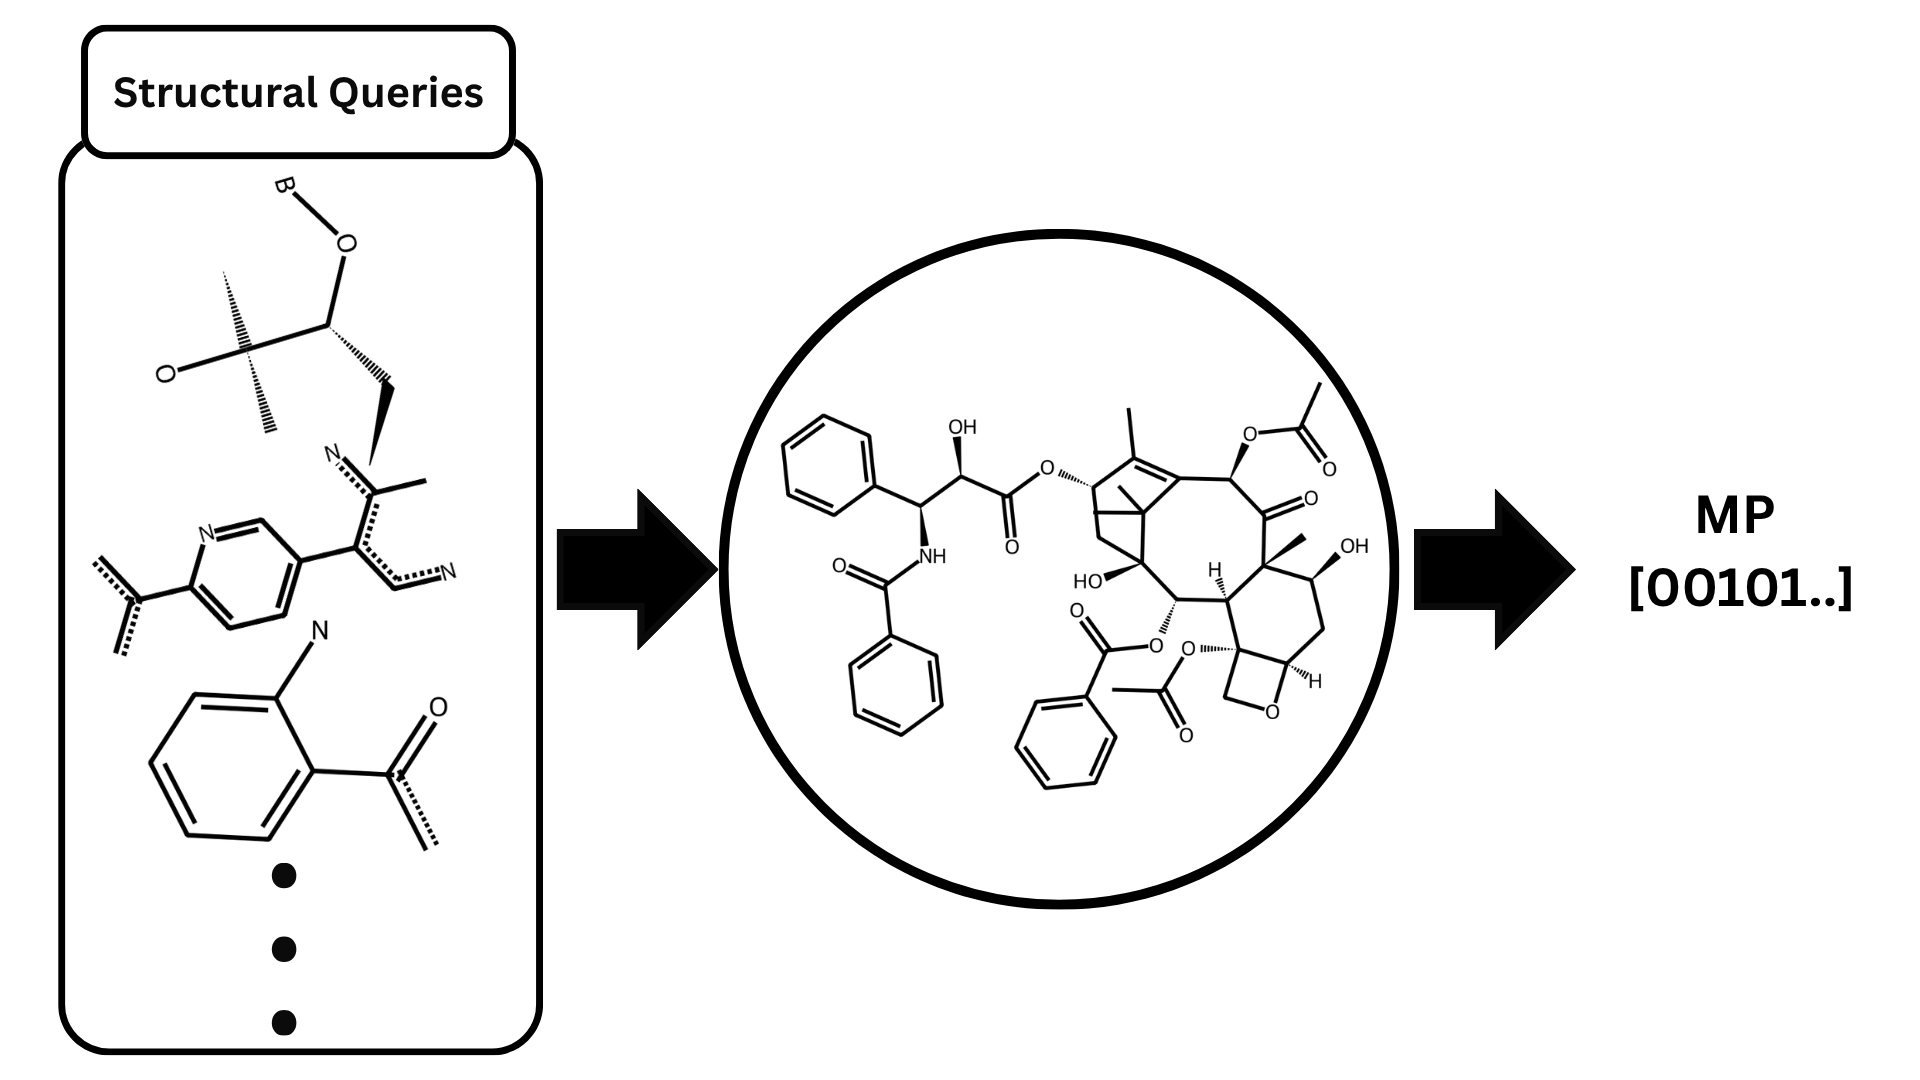
\includegraphics[scale = 0.25]{Mprofile2.png}% Replace with your image filename
	\caption{Fragmentation of target molecule to produce MFPs and MPs}
	\label{fig:mpex} % Optional: use \label for referencing
\end{figure} 

    
%after which, Morgan Fingerprinting Algorithm (MFA) parameters were set to: a) radius = 4; b) nBits = 2048; c) UseFeatures = True; and d) useChirality = True. After setting the algorithm, converted data in Mols format are feed to it which results to  generation of compounds  MP and MF. The Generated MP will become the 1-D matrix (1x2048) representation of the overall 2D-structure of each compound, which  consist of binary numbers, whereas, the MF will be the representation of molecular fingerprints/ morgan fingerprints (i.e., fragments) which were recognized as bits by the machine.

%To check if the conversion of 6304 compounds 2D-structure were successful, molecular drawing was performed through rdkit draw package. In this procedure, compounds MF's and MP's were reconverted back to its respective 2D-structures and saved as png file. In this way, the researchers were able to check the success of MP's and MF's generation via MFA. All of the data generated from these procedures were used to study the Quantitative-Structural Activity Relationship of the compounds against HCT-116.  

\subsection*{Structural Activity Relationship (SAR) of HCT-116 Compounds}
%\subsubsection{}
MFP and MP 1-D representations were used to set the ML environment. Once set, the 2D-structural data inputs can be readily perceived and interpreted by the Machine Learning Algorithm (MLA). An initial analysis of the bits was performed to categorize them before feeding to the MLA, which would allow for their assessment of significance. This is important in order to prioritize bits for subsequent feed to the MLA. When direct counting of bits was done (i.e. reflecting their absence or presence in the data set), structural queries resulted to total frequency of bits from which their ranking was based. This is the major principle in Crude Bit Counting (CBC). From the ranking, top 10 bits were used to create a CBC-ML Model, which was expected to have some capacity to predict bioactivity against HCT-116 (\autoref{fig:CBC}). On the other hand, a clustering step was also performed prior to counting, with the anticipation of shared or common features naturally emerging from the clustered molecules. This is the primary essence of Clustered Subtraction Bit Counting (CSBC).

%However, at this point there was still no way to determine which bits were significant --- there is no assessment on the weights of each bits relative to the bioactivity against HCT-116. Thus, the generated MF's were first analyzed and categorized before feeding it to the MLA. In this study, two methods were implemented to categorize and analyze the bits: CBC and CSBC.
  
%cannot identify which among the bits were significant and insignificant, hence, it lacks the ability to assess the weights of each bits relative to its bioacitivity against HCT-116. Therefore, the generated MF's were first analyzed and categorized before feeding it to the machine. In this study, two methods were implemented to categorized and analyzed the bits which are Crude Bits Counting (CBC), and Cluster-Subtraction Bits Counting (CSBC). 

\begin{figure*}[h] % 'h' places the figure approximately here
	\centering
    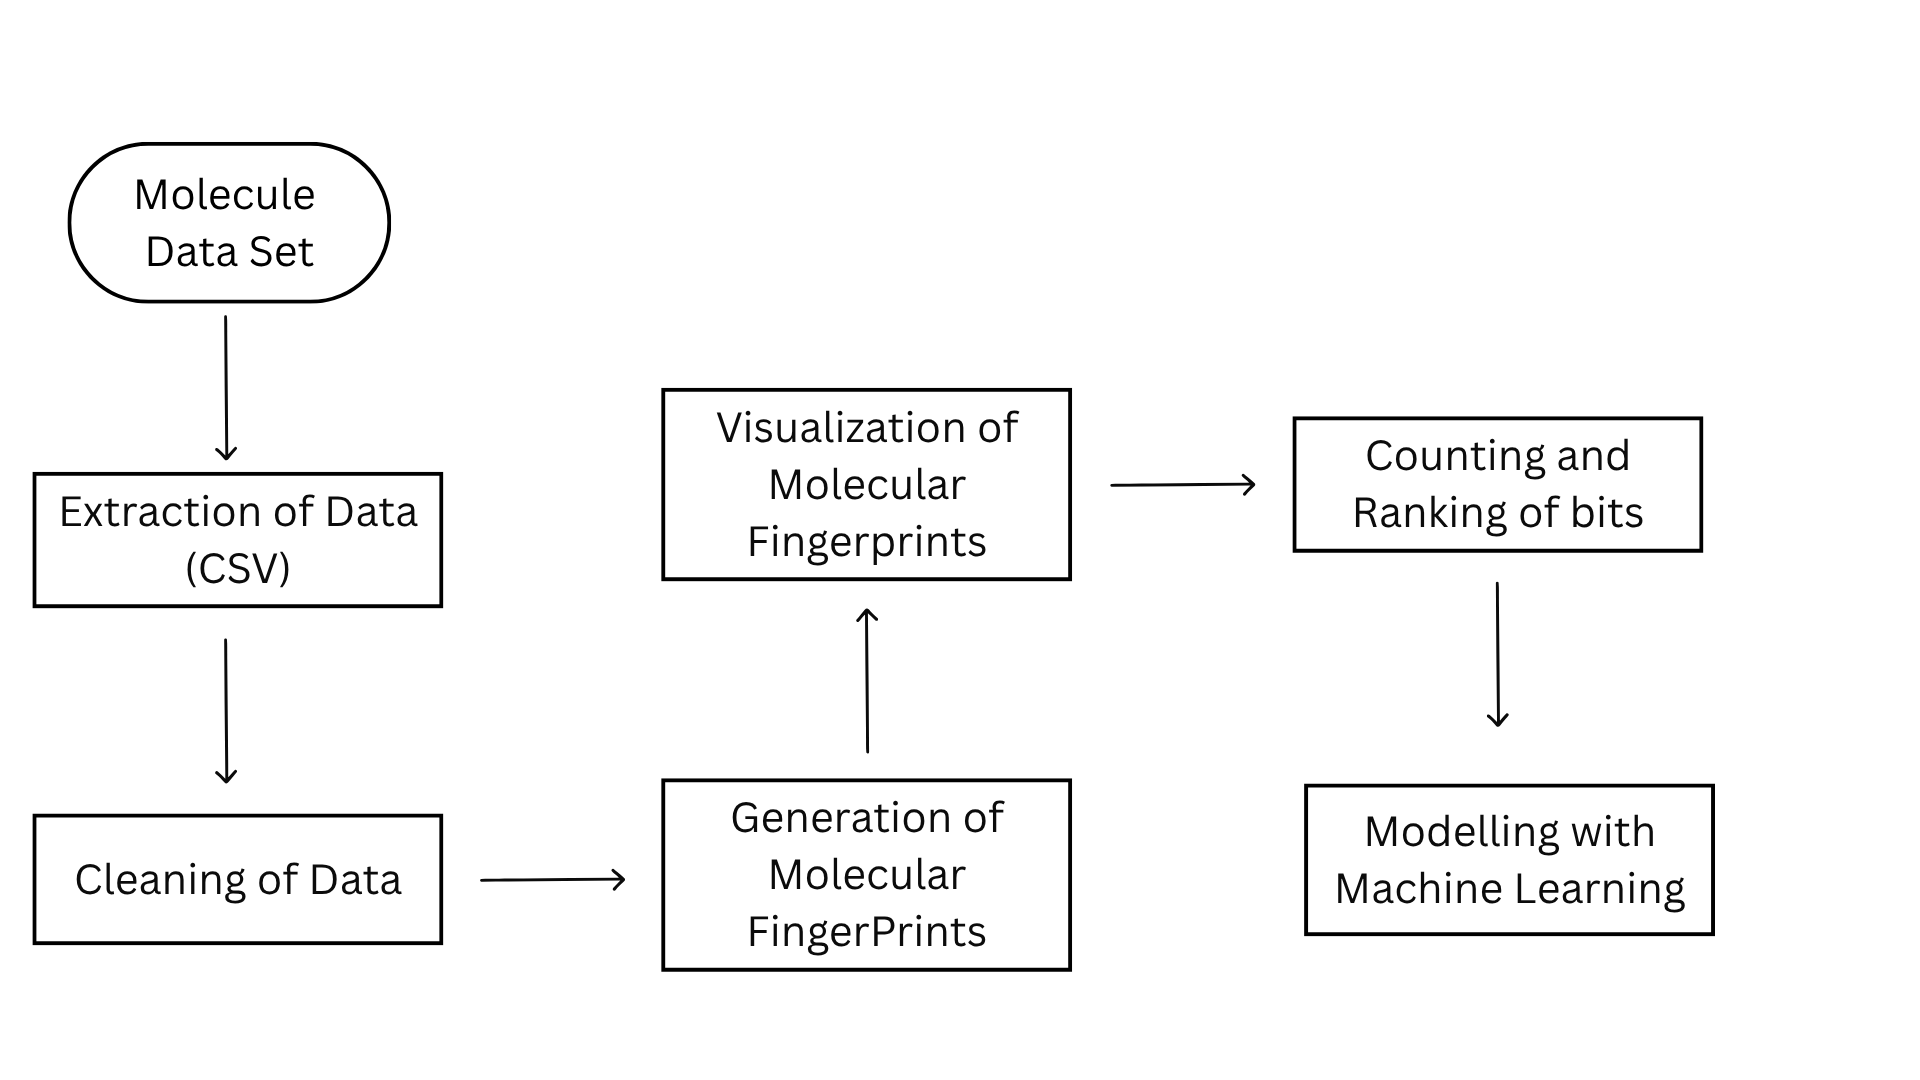
\includegraphics[scale = 0.33]{cbcv2.png}
    \vspace{-1cm} % Replace with your image filename
    \caption{Methodological framework CBC-ML}
    \label{fig:CBC} % Optional: use \label for referencing
\end{figure*}

%In CBC, after the generation and visualization of MF's and MP's, the unique bits that were produced by MFA are counted based on their presence or absence in the data set. A series of structural queries were performed to determine the total frequency of the specific bit in the given data set. After determining the total frequency of each bits, they are ranked in descending order. From the ranking, top 10 bits were used to create a CBC-ML Model, which was expected to have a capacity to perceive and classify molecules bioactivity against HCT-116 (\autoref{fig:CBC}). 

\begin{figure*}[h] % 'h' places the figure approximately here
    \centering
    \hspace{-1.05cm}
    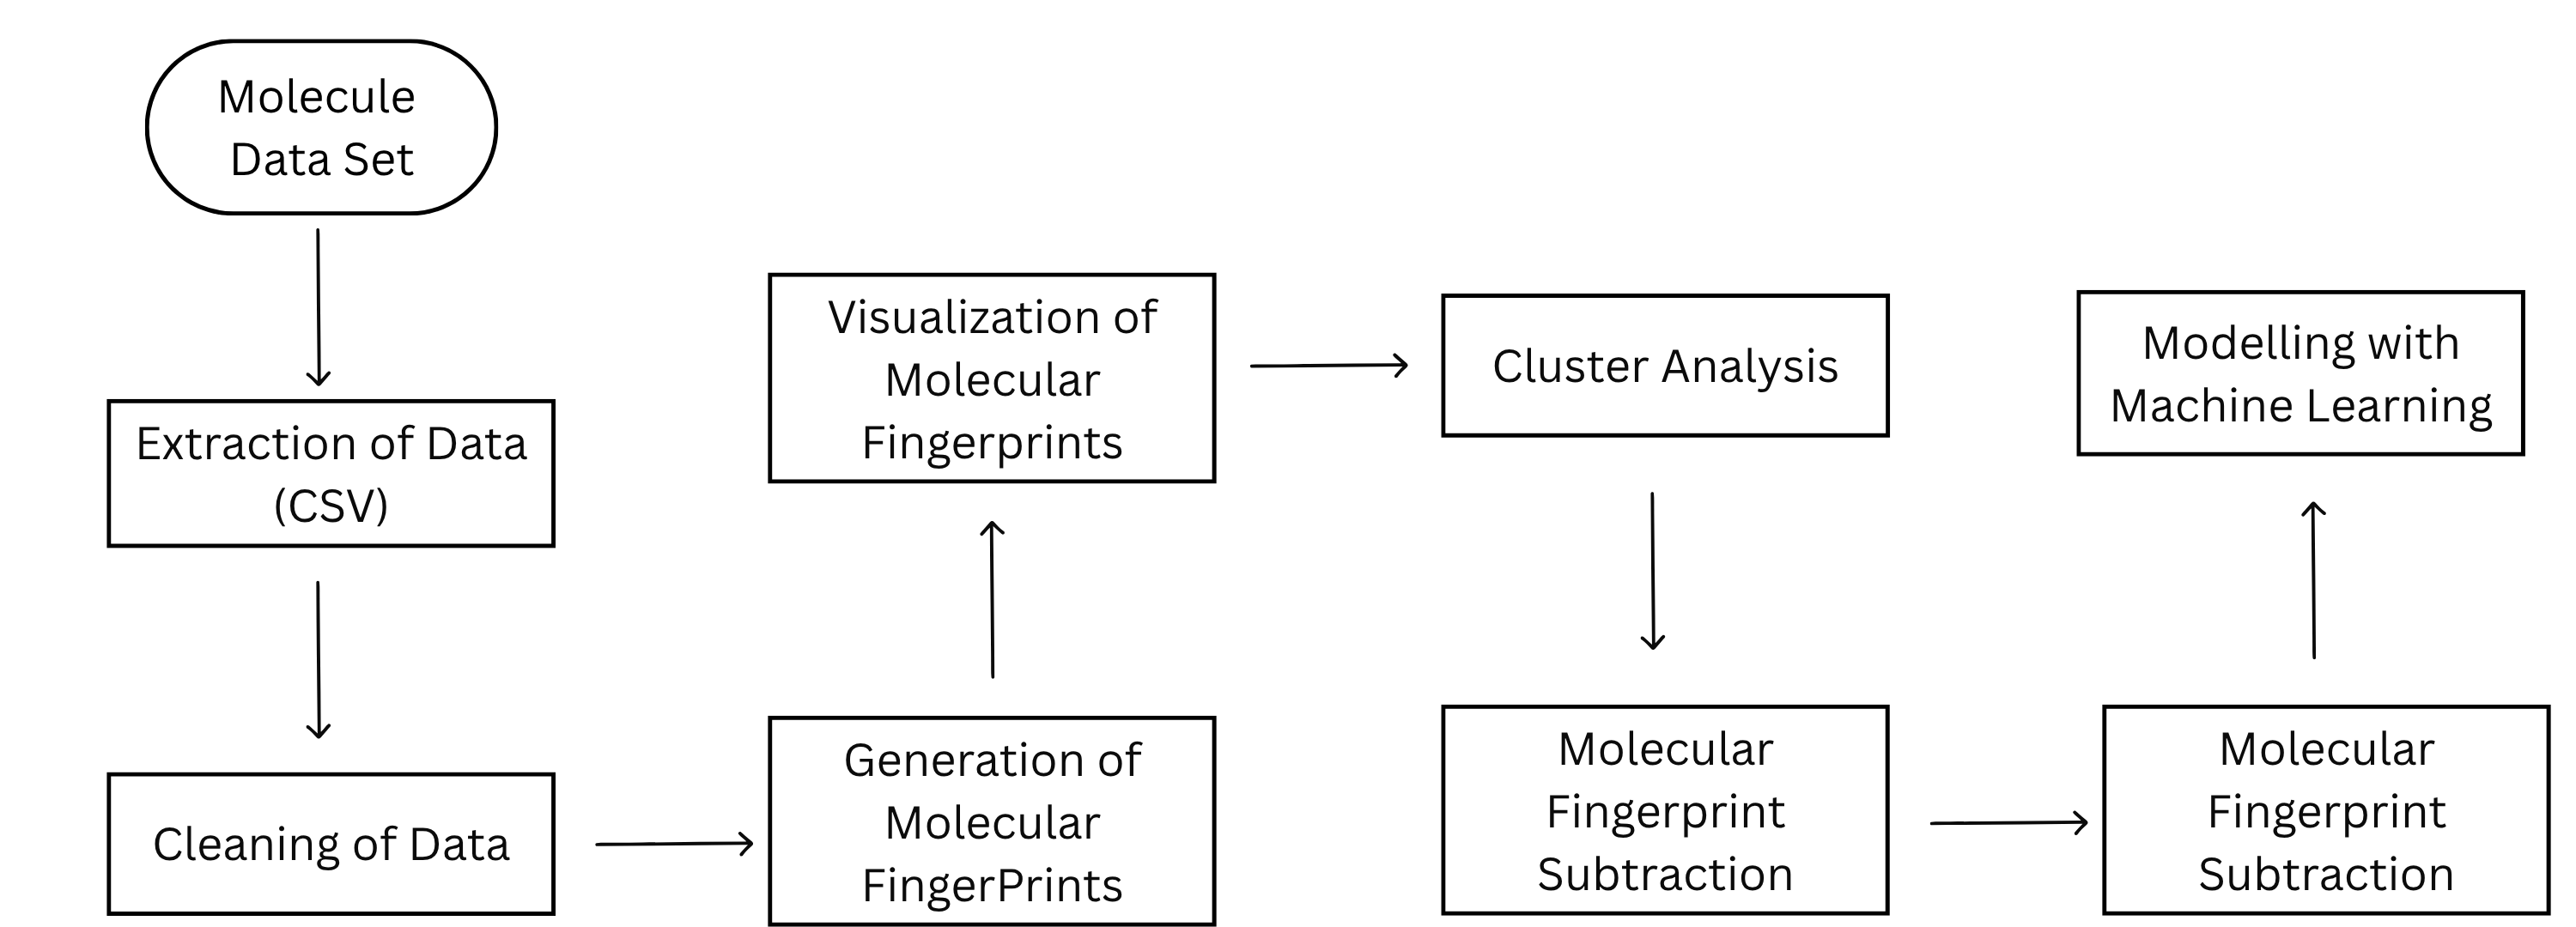
\includegraphics[scale=0.22]{csbcv2.png} % Replace with your image filename
    \caption{Methodological framework CBC-ML}
    \label{fig:CSBC} % Optional: use \label for referencing
\end{figure*}

To make sure that the optimum number of clusters was used in CSBC, Within-Cluster Sum of Squares (WCSS) (\autoref{eq:WCSS}) was computed through the elbow method. Its goal is to find the number of clusters where WCSS values converge (i.e., it does not significantly change even after increasing the number of clusters). K-Clustering was then done through the calculation of euclidean distance (\autoref{eq:euclid}) between the centroids and data points. Initially, k-seeding was performed with centroids randomly placed across the dataset. Centroid positions were then optimized based on their euclidian distances relative to a given data point (i.e., \% Inhibition). This continued until a minimum radius was achieved. The random state of the centroids in K-Clustering was set to 29. \footnote{if the random state is not set every run could have minimal variations.}

%After parameter optimization of K-Clustering it was then used to cluster clean data set of HCT-116. 

\begin{equation}
   WCSS =\sum_{i=1}^{k}\sum_{j=1}^{n_{i}}distance(x^{i}_{j},c_{i})^{2}
   \label{eq:WCSS}
\end{equation}    
where $distance(x^{i}_{j},c_{i})$ represents the distance between j-th data points $x^{i}_{j}$ in centroid $c_{i}$ and  cluster i. 

   
 \begin{equation}
    d =\sqrt{(x_{2}-x_{1})^2 +(y_{2}-y_{1})^2}
\label{eq:euclid}
\end{equation}
where d is the Euclidean distance, and $(x_{2}-x_{1}),(y_{2}-y_{1})$ are the Molecule ID and \% Inhibition respectively. 

Each cluster was then labelled under the following categories: a) High Inhibition (HI); b) Moderate Inhibition (MI); c) Low Inhibition (LI); d) Very Low Inhibition (VLI); and e) No Inhibition (NI). Since each compounds has its own MP represented by a vector, they can be added, subtracted, or multiplied. To easily categorize which among the bits were more significant than the others, MPs of compounds under VLI were subtracted from the HI, MI, LI and NI categories (\autoref{fig:subtraction}). By doing so, the bits that appear to positively contribute to the bioactivity (or positive bits, PB) the bits that negatively contribute to the bioactivity (or negative bits, NB), and the bits that appear to have no influence on bioactivity  (or non-significant bits ,NSB) were identified \footnote{PB and NB are both classified as significant bits because they positively or negatively affect the \%Inhibition of compounds against HCT-116.}. After Cluster Subtraction, the resulting vector difference underwent simplification (i.e., combination of same MPs); followed by bit frequency counting, ranking, and comparison (\autoref{fig:CSBC}). The top 16 most common bits were used for the creation of CSBC-Machine Learning Models (CSBC-ML).

\vspace{-0.55cm}
\begin{figure}[h] % 'h' places the figure approximately here
	\centering
	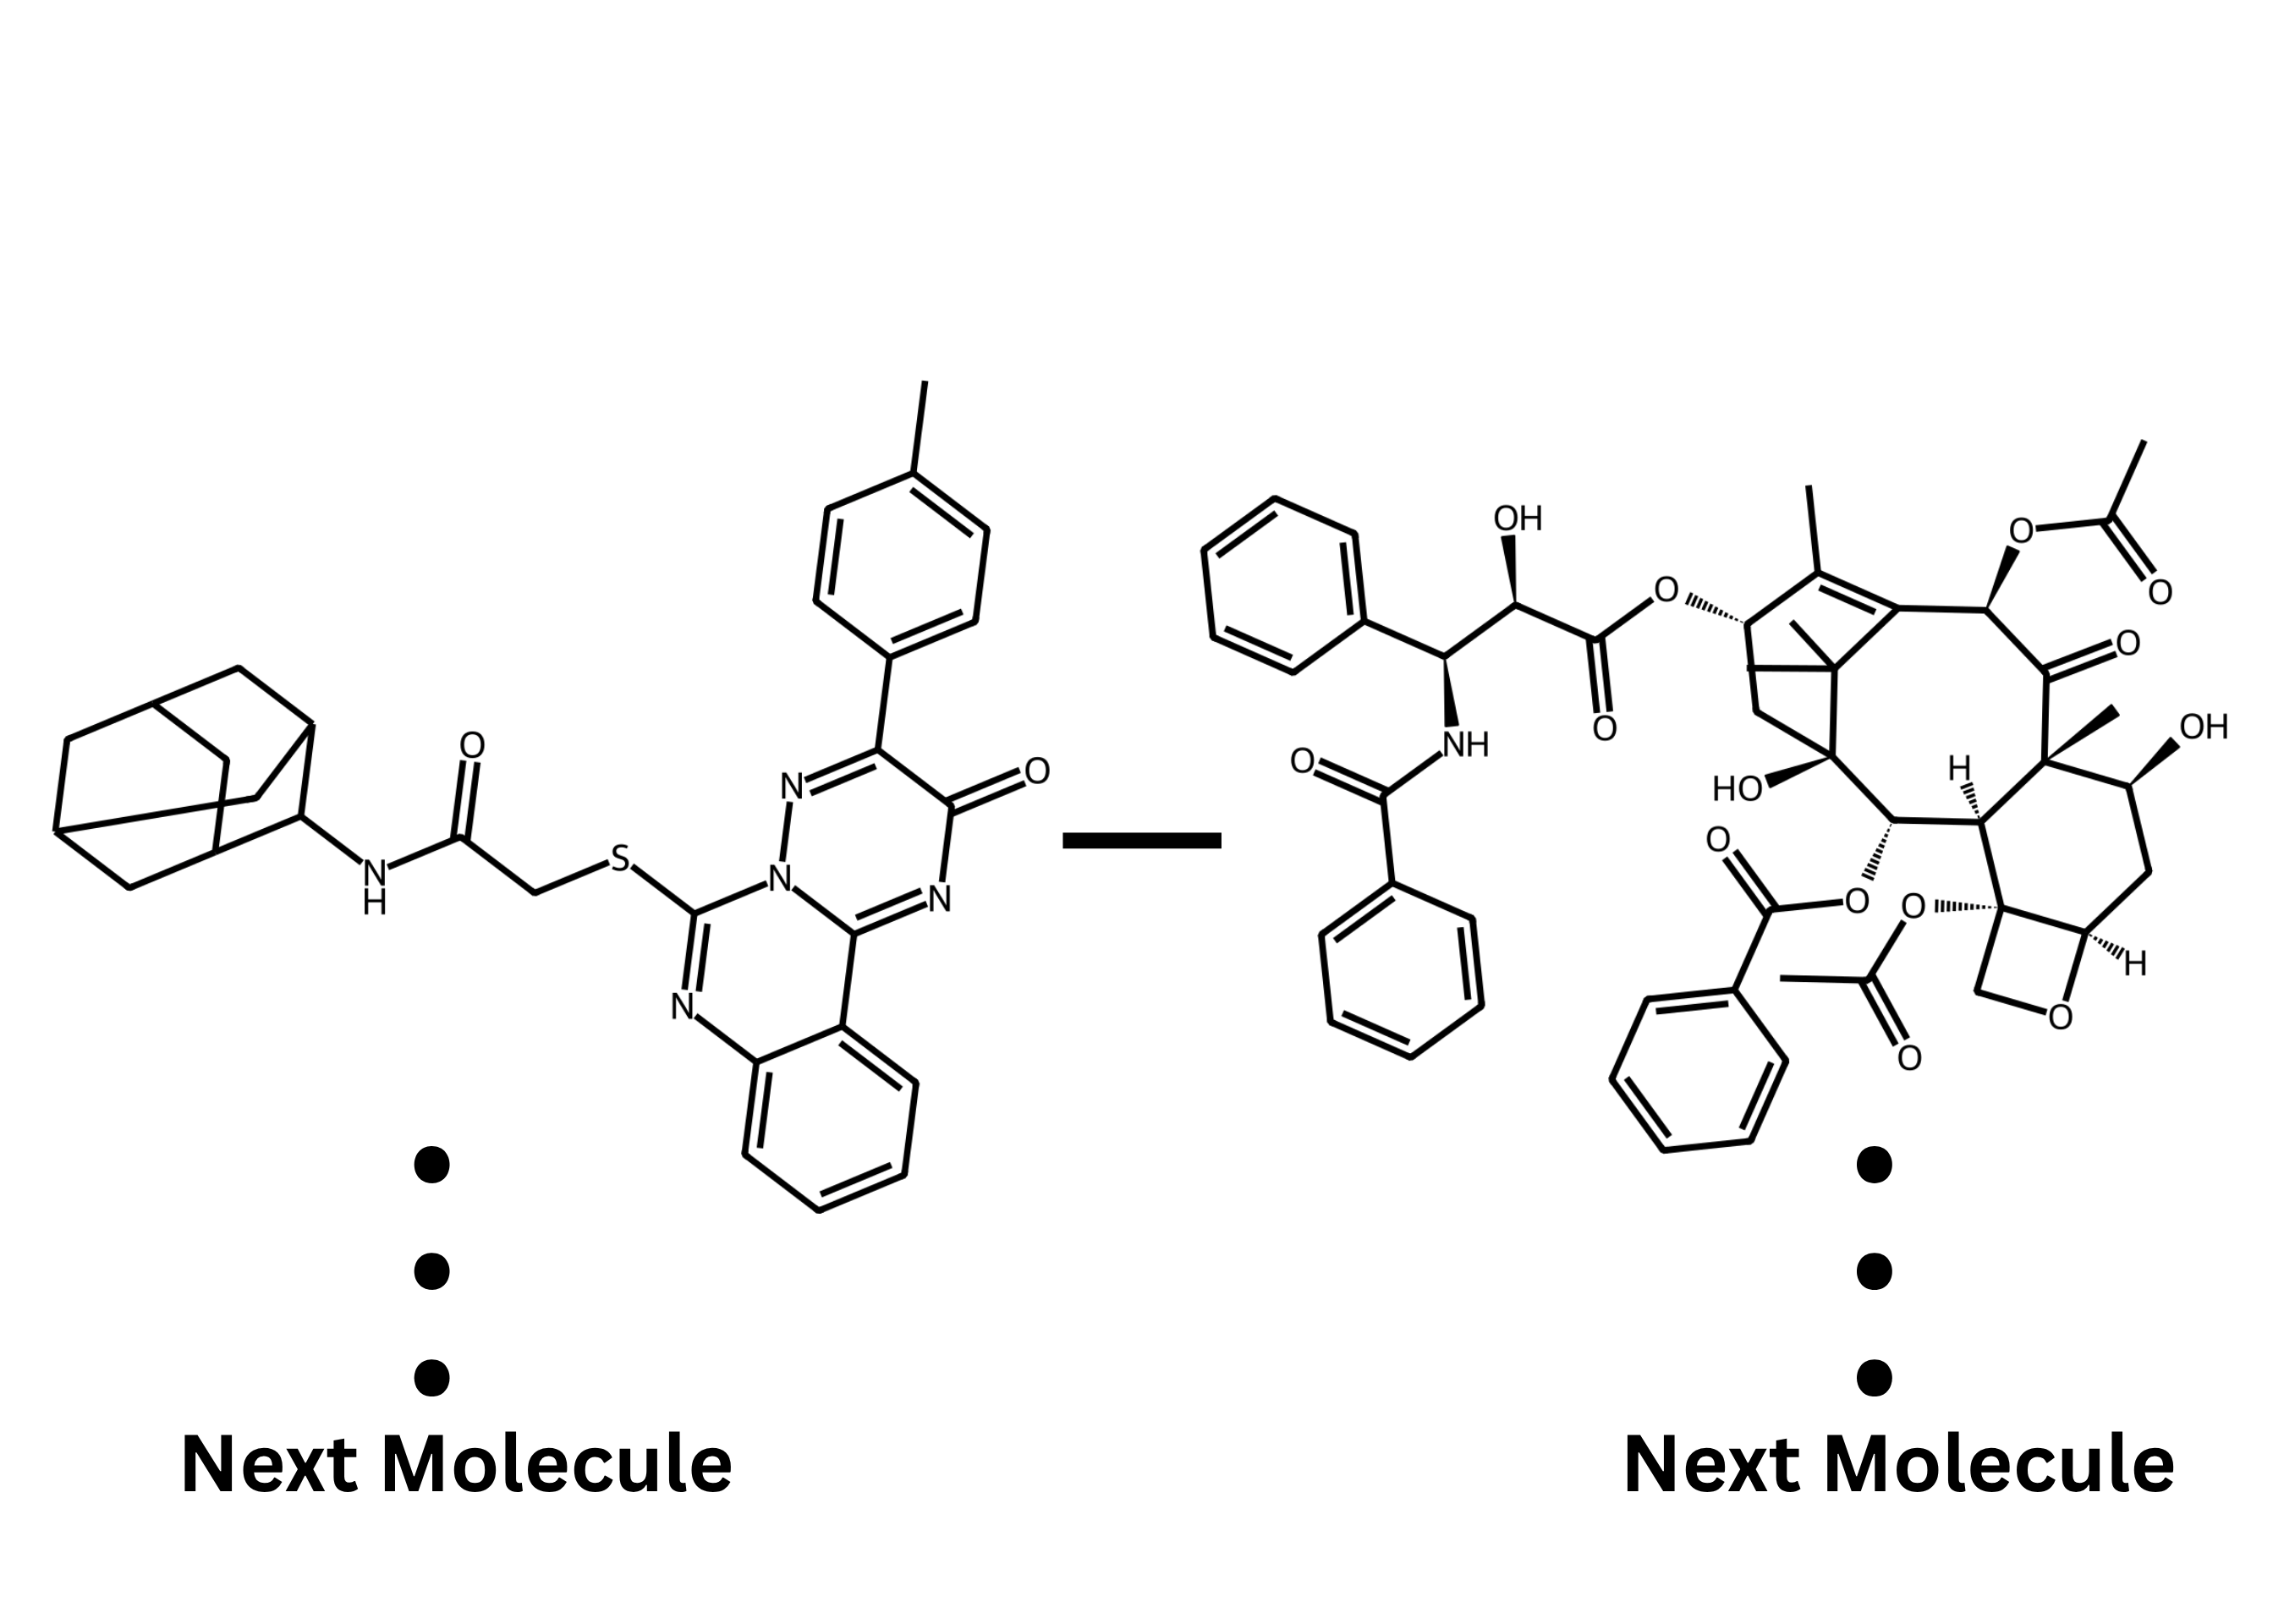
\includegraphics[width=0.57\textwidth]{mol15_minus_mol135.png} % Replace with your image filename
	\vspace{-0.5cm}
	\begin{equation*}
		\begin{bmatrix}
			1 & 0 & 1 & 0 & 1 & 1 & 1 & \ldots & 1 \\ 
			0 & 1 & 1 & 0 & 1 & 1 & 1 & \ldots & 1 \\
			\vdots & \vdots & \vdots & \vdots & \vdots & \vdots & \vdots & \ldots & \vdots \\
			0 & 1 & 1 & 0 & 1 & 1 & 1 & \ldots & 1
		\end{bmatrix}
		\text{-}
		\begin{bmatrix}
			0 & 1 & 0 & 1 & 1 & 1 & 1 & \ldots & 1 \\ 
			0 & 1 & 0 & 1 & 1 & 1 & 1 & \ldots & 1 \\
			\vdots & \vdots & \vdots & \vdots & \vdots & \vdots & \vdots & \ldots & \vdots \\
			0 & 0 & 1 & 0 & 1 & 1 & 1 & \ldots & 1
		\end{bmatrix}
		\text{=}
		\begin{bmatrix}
			1 & 0 & 1 & -1 & 0 & 0 & 0 & \ldots & 1 \\ 
			0 & 0 & 1 & -1& 0 & 0 & 0 & \ldots & 1 \\
			\vdots & \vdots & \vdots & \vdots & \vdots & \vdots & \vdots & \ldots & \vdots \\
			0 & 0 & 1 & 0 & 0 & 0 & 0 & \ldots & 1
		\end{bmatrix}
	\end{equation*}
	\caption{Structure subtraction in CSBC}
	\vspace{-0.3cm}
	\label{fig:subtraction} % Optional: use \label for referencing
\end{figure}
      
\subsection*{Quantitative Structural Activity Relationship (QSAR): CBC-ML and CSBC-ML}
The top 10, and top 16 most common structures from CBC and CSBC methods were used in the development of ML models for CBC (CBC-ML) and CSBC (CSBC-ML). These were expected to accurately perceive and classify the compounds by bioactivity against HCT-116 (active or inactive) based on their 2D-Structures. The following mathematical models were used in this study to develop the CBC-ML and CSBC-ML: a) Logistic Regression Model (Logit); b) XGBoost Model (XGB); c) Random Forest Model (RF); and d) Support Vector Machine Model (SVM) (\autoref{tab:math_models}). 

%\subsubsection*{a. CBC-ML and CSBC-ML: Mathematical Models}
\FloatBarrier % Ensures table stays below subsection

\begin{table}[h]
	\centering
	\renewcommand{\arraystretch}{1.3}
	\small
	\begin{threeparttable} % Enables footnotes
		\begin{tabular}{>{\centering\arraybackslash}p{2cm} >{\centering\arraybackslash}p{6cm} >{\centering\arraybackslash}p{6cm}}
			\hline
			\textbf{Mathematical Models} \cite{SML-formulas} & \textbf{Equations} & \textbf{Cases} \\
			\hline
			Logit \tnote{a} &  
			\begin{equation}
				y = \beta_0 + \beta_1X_1 + \beta_2X_2 + \ldots + \beta_nX_n + \epsilon
				\label{eq:logit}
			\end{equation} &  
			Performs well with linearly correlated data. \\  
			
			XGB \tnote{b} &  
			\begin{equation}
				\mathcal{L} = \sum_i l(y_i, \hat{y}_i) + \sum_k \Omega(f_k)
				\label{eq:xgboost}
			\end{equation} &  
			Can handle large datasets, imbalanced classes, and complex relationships. \\  
			
			RF \tnote{c} &  
			\begin{equation}
				f(x) = \frac{1}{M} \sum_{m=1}^M h_m(x)
				\label{eq:random}
			\end{equation} &  
			Works well with non-linear data, robust against noise and over-fitting. \\  
			
			SVM \tnote{d} &  
			\begin{equation}  
				\min \frac{1}{2} w^2 \quad \text{subject to } y_i(w \cdot x_i + b) \geq 1
				\label{eq:svm}
			\end{equation} &  
			Suitable for high-dimensional spaces, performs well for non-linear separable problems, and resistant to over-fitting. \\  
			\hline
		\end{tabular}
		\begin{tablenotes}
			\scriptsize
			\item[a] $ y $ is the target variable (\% Inhibition), $\beta_0$ is the intercept, $\beta_n$ are coefficients, and $\epsilon$ is the error term.
			\item[b] $ l(y_i, \hat{y}_i) $ is the loss function, and $ \Omega(f_k) $ is the regularization term controlling model complexity.
			\item[c] $ M $ is the total number of trees, and $ h_m(x) $ is the output from tree $ m $.
			\item[d] $ w $ is the weight vector defining the hyperplane, $ x_{i} $ are input features, $ y_{i} $ are target labels (\% Inhibition against HCT-116), and $ b $ is the bias term.
		\end{tablenotes}
	\end{threeparttable}
	\caption{Comparison of mathematical models, their underlying equations, and applicability}
	\label{tab:math_models}
\end{table}

\FloatBarrier % Prevents table from floating too far

Logit models focus (\autoref{eq:logit}) on identifying the presence and absence of a specific feature in a given query. It is based on minimizing the residual sum of squares to find the optimal parametric weights for the features. However, the Logit algorithm only works for a linearly behaved data set. For non-linear behavior, XGB, RF and SVM are best to implement due to the following reasons: a) XGB (\autoref{eq:xgboost}) involves gradient boosting iteration that gives its advantage on improving its predictions by correcting residuals during the learning process; b) RF models builds an ensemble of decision trees that are averaged to lead to a prediction; and c) SVM model finds the optimal hyperplane between the target features and its variables by adjusting its kernel functions $(K(x,x'))$(\ref{eq:svm}). The dataset used in the model development was partitioned in an 80-20 split with a random state of 29.

%\subsubsection*{a. Logit Model of CBC-ML and CSBC-ML}
%Logit Models focuses (\ref{eq:logit}) on identifying the presence and absence of a specific feature in a given query. The model is based on minimizing the residual sum of squares to find the optimal parameteric weights for the features. Fundamentally, CBC-ML and CSBC-ML were designed to accurately locate the target features (bits) in a given query (2-D structure of compounds), and to determine its specific weights. The two top bits resulting from the CBC or CSBC method were used as the features for  the CBC-ML and CSBC-ML respectively. To train and test the models, clean data set was split into train and test groups via an 80-20 partition. The models produced from this procedure are named accordingly as CBC-ML-LOG and CSBC-ML-LOG. 
%To achieved the consistency in every runs, the random state is set to 29. 

%In the training sets, the models were trained to perceived and calculate the weights of each target features, and used them to predict the compounds potency against HCT-116. Whereas, test data set were used to validate the prediction produced by the model.     

%where y is the target variable (\% Inhibition), $\beta_0$ is the intercept, ($\beta_1$, $\beta_2$ , $\ldots$, and $\beta_n$) coefficients of each features (MF/bits),($X_1$, $X_2$, $\ldots$, $X_n$) are input features (i.e., 1 & 0) and $\epsilon$ is the random error term. 

%\subsubsection*{b. XGBoost Model of CBC-ML and CSBC-ML}
%In case that the features were not linearly correlated to the target variable (\%Inhibition against HCT-116), XGBoost model were employed (\ref{eq:xgboost}). This model involves gradient boosting iteration that gives its advantage on improving its predictions by correcting residuals during the learning process. Features used in this model were the same as the Logit model and the random state was set to 29. For the development of CBC-ML-XGB and CSBC-XGB, clean data set were partitioned into 80-20 (training, testing), and the features used are the top bits from CBC and CSBC respectively.    


%where ($l(y_i, \hat{y}_i)$) is the Loss function (e.g., Mean Squared Error or Log Loss) and ($\Omega(f_k)$) is Regularization term to control model complexity. 


%\subsubsection*{c. Random Forest Model of CBC-ML and CSBC-ML}
%Random Forest Model are also effective on handling non-linear data and known to be robust against noise and overfitting (\ref{eq:random}). It builds an ensemble of decision tree that are averaged to produced a prediction. Since, the top bits could have multicollinearity characteristics, it could be detected through Random Forest Model. However, compared to Logit and XGBoost models, it is computationally intensive. For the development of CBC-ML-RF and CSBC-ML-RF, clean data set were partitioned by 80-20 with a random state of 29, and the features used were the top bits from CBC and CSBC. 


%where (M) is the total number of trees, and ($h_m(x)$) is output from tree (m). 


%\subsubsection*{d. Support Vector Machine Model of CBC-ML and CSBC-ML}
%The features used in this study were the top bits which probably have high-dimensionality, if this is the case, SVM model fits the best. SVM model aims to find the optimal hyperplane between the target features and variable. In instances of non-linearity behavior, the model kernel functions ($K(x, x')$) can be adjusted to transform the feature space (\ref{eq:svm}), making it possible for the model to handle complex and high-dimensionality data sets. However, compared to other models presented, it is memory intensive and hard to interpret. The model produced from this mathematical model were called CBC-ML-SVM and CSBC-ML-SVM, wherein the partitioned clean data set and top bits were used as the target labels and input features respectively. 


%where (w) is weight vector defining the hyperplane, ($x_{i}$) are input features, ($y_{i}$) target labels (\%Inhibition against HCT-116) and (b) is the bias term. 

\subsubsection*{Comparative Analysis of QSAR-ML Models}
Results from the four different models were assessed based on the following: a) accuracy and precision through a confusion matrix; b) model fitting of performance during training and testing; and c) overall ability of the model to distinguish between classes. The confusion matrix is a performance evaluation tool that can assess how well a model has predicted outcomes based on comparing the actual positive and negative to predicted values. It entails information about accuracy, precision, recall (sensitivity), F1 score, and specificity(\autoref{eq:accu} - \ref{eq:speci}). 

\begin{equation}
    \text{Accuracy} = \frac{\text{TP} + \text{TN}}{\text{TP} + \text{TN} + \text{FP} + \text{FN}}
    \label{eq:accu}
\end{equation}

\begin{equation}
    \text{Precision} = \frac{\text{TP}}{\text{TP} + \text{FP}}
    \label{eq:prec}
\end{equation}

\begin{equation}
   \text{Recall} = \frac{\text{TP}}{\text{TP} + \text{FN}}
   \label{eq:recall}
\end{equation}

\begin{equation}
     \text{F1 Score} = 2 \cdot \frac{\text{Precision} \cdot \text{Recall}}{\text{Precision} + \text{Recall}}
     \label{eq:f1}
\end{equation}

\begin{equation}
    \text{Specificity} = \frac{\text{TN}}{\text{TN} + \text{FP}}
    \label{eq:speci}
\end{equation}

where (TP, TN) are the true positive and true negative values, while (FP, FN) are the false positive and false negative values.

To check the performance fit of each model, the confusion matrix parameters were compared during the training and the testing stages. To evaluate the overall capability of the model to distinguish between classes (active and inactive against HCT-116), ROC, and AUC (\autoref{eq:tpr} - \ref{eq:auc}) were used. AUC helps to summarize the results from the ROC curve using the following criterion: a) AUC = 1.0 perfect classification; and b) AUC = 0.5 random guessing (no discriminatory power). A good model is expected to have the following: a) high accuracy and precision; b) a good fit (not over- or under-fitted); and c) an AUC value greater than 0.5. 

\begin{equation}
    \text{TPR} = \frac{\text{TP}}{\text{TP} + \text{FN}}
    \label{eq:tpr}
\end{equation}

\begin{equation}
    \text{FPR} = \frac{\text{FP}}{\text{FP} + \text{TN}}
    \label{eq:fpr}
\end{equation}

\begin{equation}
    \text{AUC} = \int_{0}^{1} \text{TPR}(\text{FPR}) , d(\text{FPR})
    \label{eq:auc}
\end{equation}
where TPR and FPR are the true and false positive rates.
%\subsubsection{}



	
	%\chapter{ACKNOWLEDGMENTS}
	%	\input{acknowledgement}
	
	%\chapter{Appendix}
	%	\subsection*{A. Top bits Summary from CBC and CSBC Methods}

\subsubsection{1. Raw data of CBC Top 10 bit frequency}
\FloatBarrier
\begin{table}[h]
	\centering
	\begin{threeparttable}
		\renewcommand{\arraystretch}{1.2} % Adjust row spacing
		\small
		\begin{tabular}{>{\centering\arraybackslash}p{3cm} >{\centering\arraybackslash}p{3cm}}  
			\hline
			\textbf{Bit\_{ID} \tnote{b}} & \textbf{Frequency} \\  
			\hline
			0 & 6140 \\  
			2 & 6086 \\  
			4 & 5982 \\  
			2017 & 5805 \\  
			2040 & 5250 \\  
			428 & 4643 \\  
			6 & 4124 \\  
			1556 & 3586 \\  
			1155 & 3450 \\  
			598 & 3446 \\  
			\hline
		\end{tabular}
		\begin{tablenotes}
			\item[b] contains the Molecular Fingerprint ID generated in MFA
		\end{tablenotes}
	\end{threeparttable}
	\caption{Top 10 Bits: Generated Through CBC Method}
	\label{tab:t10crude}
\end{table}
\FloatBarrier

\subsubsection{2. Raw data of CSBC Most Common bit frequency}
\FloatBarrier
\begin{table}[H]
	\centering
	\small
	\renewcommand{\arraystretch}{0.7} % Adjust row spacing
	\begin{threeparttable}
		\begin{tabular}{p{1cm} p{2cm} p{1cm} p{2cm} p{1cm} p{2cm} p{1cm} p{2cm}}
			\hline
			AB \tnote{c} & Frequency & AC & Frequency & AD & Frequency & AE & Frequency \\ 
			\hline
			598  & 767936 & 1556.0 & 15920.0 & 1556.0 & 15600.0 & 857.0  & 2916.0  \\  
			1556 & 673190 & 598.0  & 14782.0 & 1.0    & 14993.0 & 839.0  & 1972.0  \\  
			857  & 669664 & 1155.0 & 14615.0 & 598.0  & 14896.0 & 1155.0 & 1924.0  \\  
			1990 & 653994 & 8.0    & 14526.0 & 8.0    & 14094.0 & 1217.0 & 1922.0  \\  
			1155 & 616200 & 6.0    & 13560.0 & 1155.0 & 13616.0 & 1008.0 & 1768.0  \\  
			1085 & 611846 & 1.0    & 13536.0 & 792.0  & 13338.0 & 1990.0 & 1764.0  \\  
			1    & 609248 & 857.0  & 13014.0 & 6.0    & 12720.0 & 6.0    & 1710.0  \\  
			2039 & 606672 & 1723.0 & 12834.0 & 428.0  & 12450.0 & 805.0  & 1702.0  \\  
			792  & 603936 & 428.0  & 12725.0 & 1085.0 & 12144.0 & 1731.0 & 1675.0  \\  
			1083 & 602408 & 2044.0 & 12342.0 & 1723.0 & 11966.0 & 835.0  & 1650.0  \\  
			51   & 595882 & 1373.0 & 12338.0 & 806.0  & 11715.0 & 485.0  & 1650.0  \\  
			1863 & 593712 & 2039.0 & 12042.0 & 3.0    & 11660.0 & 792.0  & 1638.0  \\  
			6    & 591448 & 3.0    & 11766.0 & 2039.0 & 11502.0 & 232.0  & 1632.0  \\  
			19   & 585936 & 1915.0 & 11418.0 & 691.0  & 11457.0 & 1083.0 & 1617.0  \\  
			8    & 576194 & 1917.0 & 11382.0 & 1850.0 & 11395.0 & 1723.0 & 1612.0  \\  
			428  & 572000 & 1085.0 & 11362.0 & 2044.0 & 11352.0 & 1085.0 & 1610.0  \\  
			1917 & 565438 & 792.0  & 11271.0 & 1373.0 & 11346.0 & 428.0  & 1600.0  \\  
			1217 & 551670 & 51.0   & 10965.0 & 857.0  & 11340.0 & 1556.0 & 1600.0  \\  
			1219 & 545458 & 19.0   & 10962.0 & 1990.0 & 11268.0 & 1863.0 & 1575.0  \\  
			837  & 533484 & 1863.0 & 10530.0 & 1083.0 & 10890.0 & 3.0    & 1537.0  \\  
			\hline
		\end{tabular}
		\vspace{-0.3cm}
		\begin{tablenotes}
			\item[c] A: VLI, B: HI, C: MI, D:LI, E:NI 
		\end{tablenotes}
	\end{threeparttable}
	\caption{Bit Frequency Across Different Conditions}
	\label{tab:bit_frequencies}
\end{table}
\FloatBarrier


	
	
	% Ensure Bibliography starts on a new page
	\clearpage
	{\normalsize % Set font size for bibliography content
		\bibliographystyle{plain} % Bibliography style
		\bibliography{references}  % Reference to your .bib file
	}
	%%%%%%%%%%%%%%%%%%%%%%%%%%%%%%%%%%%%%%%%%%%%%%%%%%%%%%%%%%%%%%%%%%%%%
	%% The "tocentry" environment can be used to create an entry for the
	%% graphical table of contents. It is given here as some journals
	%% require that it is printed as part of the abstract page. It will
	%% be automatically moved as appropriate.
	%%%%%%%%%%%%%%%%%%%%%%%%%%%%%%%%%%%%%%%%%%%%%%%%%%%%%%%%%%%%%%%%%%%%%
	
	\begin{tocentry}
		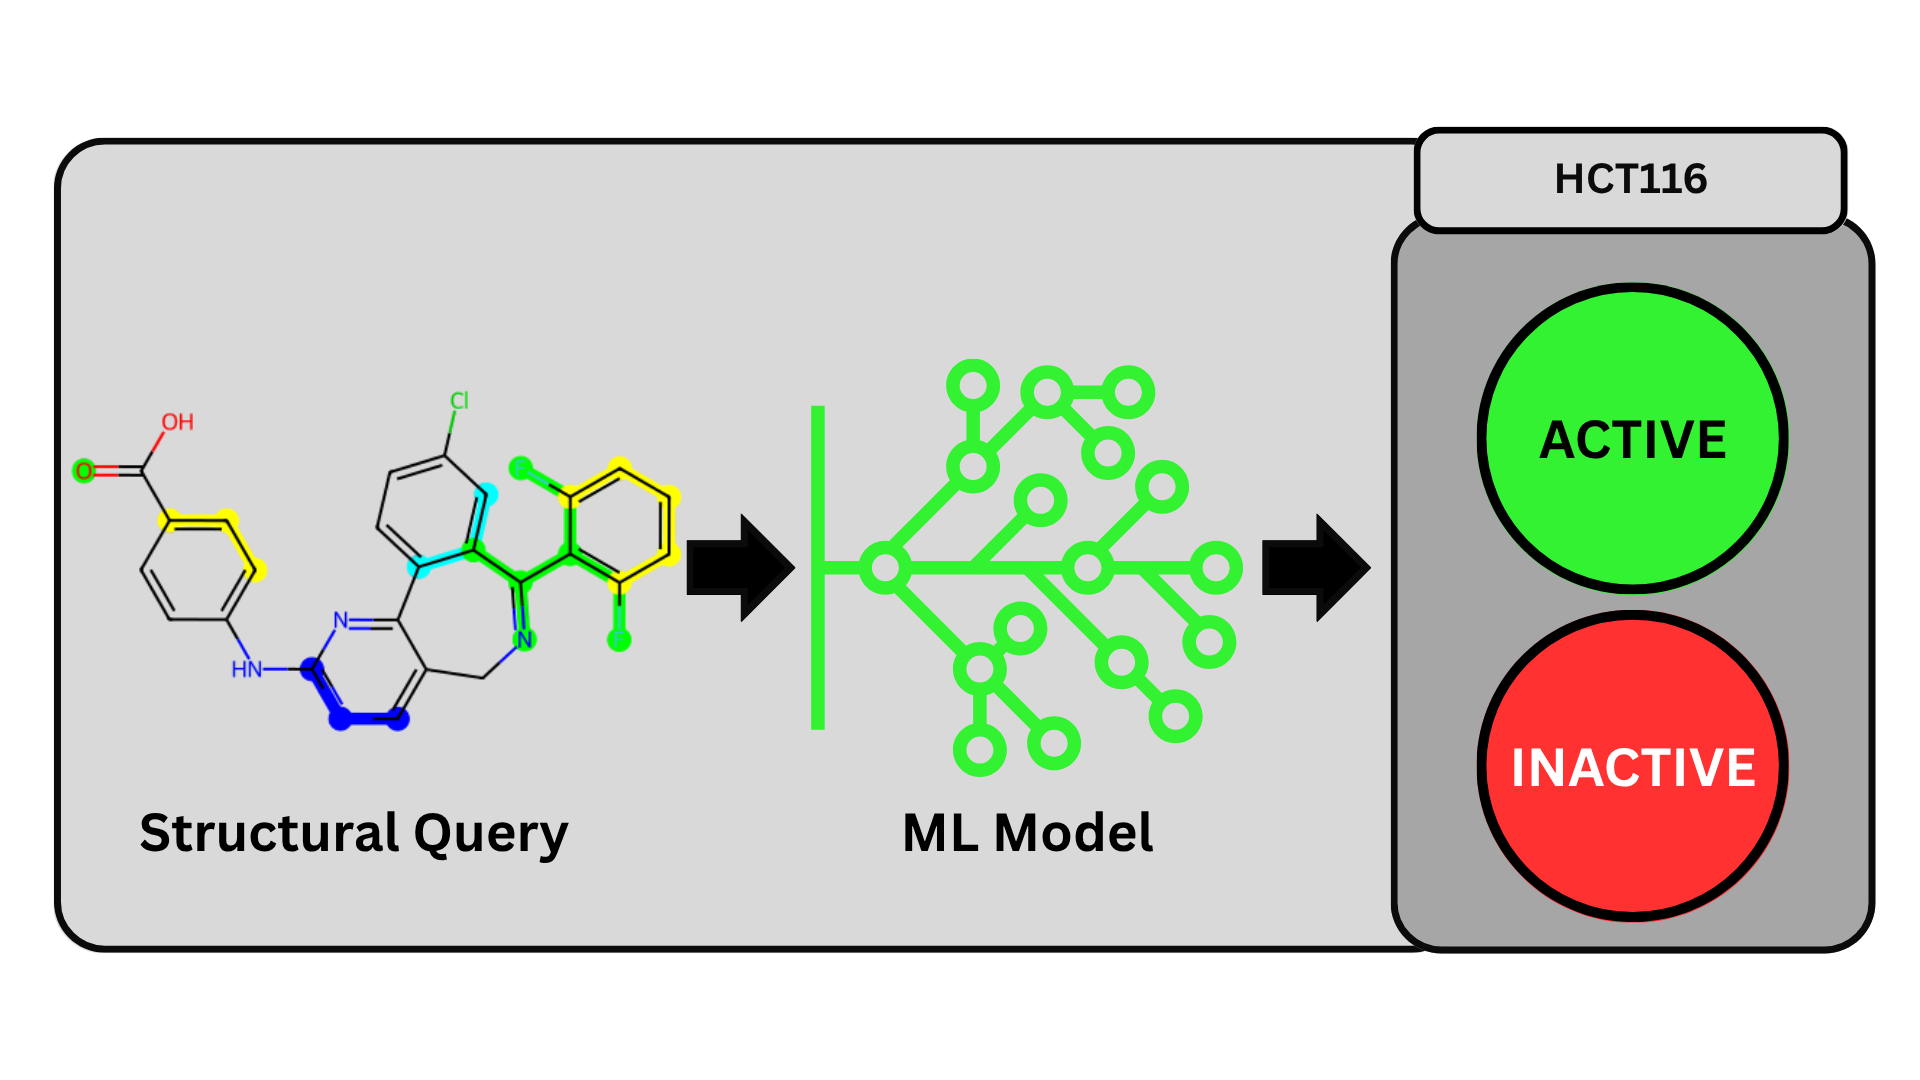
\includegraphics[width=8.5cm,height=4.75cm]{TOC_graphical.png}
	\end{tocentry}
	
		
		\begin{suppinfo}
		
		Supplementary figures, raw data and png files of bits and parent molecules can be access through this \href{https://drive.google.com/drive/u/0/folders/1eBbbIDrqLvVmLYn7Lit_3JV7y-42jcaf}{\textbf{link}}.
		
	\end{suppinfo}
	
	%%%%%%%%%%%%%%%%%%%%%%%%%%%%%%%%%%%%%%%%%%%%%%%%%%%%%%%%%%%%%%%%%%%%%
	%% The appropriate \bibliography command should be placed here.
	%% Notice that the class file automatically sets \bibliographystyle
	%% and also names the section correctly.
	%%%%%%%%%%%%%%%%%%%%%%%%%%%%%%%%%%%%%%%%%%%%%%%%%%%%%%%%%%%%%%%%%%%%%
	\bibliography{achemso-demo}
	
\end{document}